% Options for packages loaded elsewhere
\PassOptionsToPackage{unicode}{hyperref}
\PassOptionsToPackage{hyphens}{url}
\PassOptionsToPackage{dvipsnames,svgnames,x11names}{xcolor}
%
\documentclass[
  ignorenonframetext,
  aspectratio=169]{beamer}
\usepackage{pgfpages}
\setbeamertemplate{caption}[numbered]
\setbeamertemplate{caption label separator}{: }
\setbeamercolor{caption name}{fg=normal text.fg}
\beamertemplatenavigationsymbolsempty
% Prevent slide breaks in the middle of a paragraph
\widowpenalties 1 10000
\raggedbottom
\setbeamertemplate{part page}{
  \centering
  \begin{beamercolorbox}[sep=16pt,center]{part title}
    \usebeamerfont{part title}\insertpart\par
  \end{beamercolorbox}
}
\setbeamertemplate{section page}{
  \centering
  \begin{beamercolorbox}[sep=12pt,center]{part title}
    \usebeamerfont{section title}\insertsection\par
  \end{beamercolorbox}
}
\setbeamertemplate{subsection page}{
  \centering
  \begin{beamercolorbox}[sep=8pt,center]{part title}
    \usebeamerfont{subsection title}\insertsubsection\par
  \end{beamercolorbox}
}
\AtBeginPart{
  \frame{\partpage}
}
\AtBeginSection{
  \ifbibliography
  \else
    \frame{\sectionpage}
  \fi
}
\AtBeginSubsection{
  \frame{\subsectionpage}
}

\usepackage{amsmath,amssymb}
\usepackage{iftex}
\ifPDFTeX
  \usepackage[T1]{fontenc}
  \usepackage[utf8]{inputenc}
  \usepackage{textcomp} % provide euro and other symbols
\else % if luatex or xetex
  \usepackage{unicode-math}
  \defaultfontfeatures{Scale=MatchLowercase}
  \defaultfontfeatures[\rmfamily]{Ligatures=TeX,Scale=1}
\fi
\usepackage{lmodern}
\usetheme[]{CambridgeUS}
\ifPDFTeX\else  
    % xetex/luatex font selection
\fi
% Use upquote if available, for straight quotes in verbatim environments
\IfFileExists{upquote.sty}{\usepackage{upquote}}{}
\IfFileExists{microtype.sty}{% use microtype if available
  \usepackage[]{microtype}
  \UseMicrotypeSet[protrusion]{basicmath} % disable protrusion for tt fonts
}{}
\makeatletter
\@ifundefined{KOMAClassName}{% if non-KOMA class
  \IfFileExists{parskip.sty}{%
    \usepackage{parskip}
  }{% else
    \setlength{\parindent}{0pt}
    \setlength{\parskip}{6pt plus 2pt minus 1pt}}
}{% if KOMA class
  \KOMAoptions{parskip=half}}
\makeatother
\usepackage{xcolor}
\newif\ifbibliography
\setlength{\emergencystretch}{3em} % prevent overfull lines
\setcounter{secnumdepth}{-\maxdimen} % remove section numbering

\usepackage{color}
\usepackage{fancyvrb}
\newcommand{\VerbBar}{|}
\newcommand{\VERB}{\Verb[commandchars=\\\{\}]}
\DefineVerbatimEnvironment{Highlighting}{Verbatim}{commandchars=\\\{\}}
% Add ',fontsize=\small' for more characters per line
\usepackage{framed}
\definecolor{shadecolor}{RGB}{241,243,245}
\newenvironment{Shaded}{\begin{snugshade}}{\end{snugshade}}
\newcommand{\AlertTok}[1]{\textcolor[rgb]{0.68,0.00,0.00}{#1}}
\newcommand{\AnnotationTok}[1]{\textcolor[rgb]{0.37,0.37,0.37}{#1}}
\newcommand{\AttributeTok}[1]{\textcolor[rgb]{0.40,0.45,0.13}{#1}}
\newcommand{\BaseNTok}[1]{\textcolor[rgb]{0.68,0.00,0.00}{#1}}
\newcommand{\BuiltInTok}[1]{\textcolor[rgb]{0.00,0.23,0.31}{#1}}
\newcommand{\CharTok}[1]{\textcolor[rgb]{0.13,0.47,0.30}{#1}}
\newcommand{\CommentTok}[1]{\textcolor[rgb]{0.37,0.37,0.37}{#1}}
\newcommand{\CommentVarTok}[1]{\textcolor[rgb]{0.37,0.37,0.37}{\textit{#1}}}
\newcommand{\ConstantTok}[1]{\textcolor[rgb]{0.56,0.35,0.01}{#1}}
\newcommand{\ControlFlowTok}[1]{\textcolor[rgb]{0.00,0.23,0.31}{#1}}
\newcommand{\DataTypeTok}[1]{\textcolor[rgb]{0.68,0.00,0.00}{#1}}
\newcommand{\DecValTok}[1]{\textcolor[rgb]{0.68,0.00,0.00}{#1}}
\newcommand{\DocumentationTok}[1]{\textcolor[rgb]{0.37,0.37,0.37}{\textit{#1}}}
\newcommand{\ErrorTok}[1]{\textcolor[rgb]{0.68,0.00,0.00}{#1}}
\newcommand{\ExtensionTok}[1]{\textcolor[rgb]{0.00,0.23,0.31}{#1}}
\newcommand{\FloatTok}[1]{\textcolor[rgb]{0.68,0.00,0.00}{#1}}
\newcommand{\FunctionTok}[1]{\textcolor[rgb]{0.28,0.35,0.67}{#1}}
\newcommand{\ImportTok}[1]{\textcolor[rgb]{0.00,0.46,0.62}{#1}}
\newcommand{\InformationTok}[1]{\textcolor[rgb]{0.37,0.37,0.37}{#1}}
\newcommand{\KeywordTok}[1]{\textcolor[rgb]{0.00,0.23,0.31}{#1}}
\newcommand{\NormalTok}[1]{\textcolor[rgb]{0.00,0.23,0.31}{#1}}
\newcommand{\OperatorTok}[1]{\textcolor[rgb]{0.37,0.37,0.37}{#1}}
\newcommand{\OtherTok}[1]{\textcolor[rgb]{0.00,0.23,0.31}{#1}}
\newcommand{\PreprocessorTok}[1]{\textcolor[rgb]{0.68,0.00,0.00}{#1}}
\newcommand{\RegionMarkerTok}[1]{\textcolor[rgb]{0.00,0.23,0.31}{#1}}
\newcommand{\SpecialCharTok}[1]{\textcolor[rgb]{0.37,0.37,0.37}{#1}}
\newcommand{\SpecialStringTok}[1]{\textcolor[rgb]{0.13,0.47,0.30}{#1}}
\newcommand{\StringTok}[1]{\textcolor[rgb]{0.13,0.47,0.30}{#1}}
\newcommand{\VariableTok}[1]{\textcolor[rgb]{0.07,0.07,0.07}{#1}}
\newcommand{\VerbatimStringTok}[1]{\textcolor[rgb]{0.13,0.47,0.30}{#1}}
\newcommand{\WarningTok}[1]{\textcolor[rgb]{0.37,0.37,0.37}{\textit{#1}}}

\providecommand{\tightlist}{%
  \setlength{\itemsep}{0pt}\setlength{\parskip}{0pt}}\usepackage{longtable,booktabs,array}
\usepackage{calc} % for calculating minipage widths
\usepackage{caption}
% Make caption package work with longtable
\makeatletter
\def\fnum@table{\tablename~\thetable}
\makeatother
\usepackage{graphicx}
\makeatletter
\def\maxwidth{\ifdim\Gin@nat@width>\linewidth\linewidth\else\Gin@nat@width\fi}
\def\maxheight{\ifdim\Gin@nat@height>\textheight\textheight\else\Gin@nat@height\fi}
\makeatother
% Scale images if necessary, so that they will not overflow the page
% margins by default, and it is still possible to overwrite the defaults
% using explicit options in \includegraphics[width, height, ...]{}
\setkeys{Gin}{width=\maxwidth,height=\maxheight,keepaspectratio}
% Set default figure placement to htbp
\makeatletter
\def\fps@figure{htbp}
\makeatother

\usepackage{colortbl}
\usepackage{amsmath,color,array,booktabs,algorithm2e}
 \usepackage{mathdots}
 %\usepackage{yhmath}
 %\usepackage{MnSymbol}



 \definecolor{LightBlue}{RGB}{173,216,230}
 \newcommand\blue[1]{\textcolor{blue}{#1}}
 \newcommand\red[1]{\textcolor{red}{#1}}
 \newcommand\green[1]{\textcolor{green}{#1}}

\renewcommand{\contentsname}{Índice}
\renewcommand{\chaptername}{Parte}
\renewcommand{\sectionname}{Lección}
\AtBeginDocument{\title[Tema 3 Parte I: Dist. Discretas ]{Tema 3 Parte I: Distribuciones Notables Discretas}}
\makeatletter
\makeatother
\makeatletter
\makeatother
\makeatletter
\@ifpackageloaded{caption}{}{\usepackage{caption}}
\AtBeginDocument{%
\ifdefined\contentsname
  \renewcommand*\contentsname{Tabla de contenidos}
\else
  \newcommand\contentsname{Tabla de contenidos}
\fi
\ifdefined\listfigurename
  \renewcommand*\listfigurename{Listado de Figuras}
\else
  \newcommand\listfigurename{Listado de Figuras}
\fi
\ifdefined\listtablename
  \renewcommand*\listtablename{Listado de Tablas}
\else
  \newcommand\listtablename{Listado de Tablas}
\fi
\ifdefined\figurename
  \renewcommand*\figurename{Figura}
\else
  \newcommand\figurename{Figura}
\fi
\ifdefined\tablename
  \renewcommand*\tablename{Tabla}
\else
  \newcommand\tablename{Tabla}
\fi
}
\@ifpackageloaded{float}{}{\usepackage{float}}
\floatstyle{ruled}
\@ifundefined{c@chapter}{\newfloat{codelisting}{h}{lop}}{\newfloat{codelisting}{h}{lop}[chapter]}
\floatname{codelisting}{Listado}
\newcommand*\listoflistings{\listof{codelisting}{Listado de Listados}}
\makeatother
\makeatletter
\@ifpackageloaded{caption}{}{\usepackage{caption}}
\@ifpackageloaded{subcaption}{}{\usepackage{subcaption}}
\makeatother
\makeatletter
\@ifpackageloaded{tcolorbox}{}{\usepackage[skins,breakable]{tcolorbox}}
\makeatother
\makeatletter
\@ifundefined{shadecolor}{\definecolor{shadecolor}{rgb}{.97, .97, .97}}
\makeatother
\makeatletter
\makeatother
\makeatletter
\ifdefined\Shaded\renewenvironment{Shaded}{\begin{tcolorbox}[breakable, sharp corners, borderline west={3pt}{0pt}{shadecolor}, boxrule=0pt, interior hidden, enhanced, frame hidden]}{\end{tcolorbox}}\fi
\makeatother
\makeatletter
\makeatother
\ifLuaTeX
\usepackage[bidi=basic]{babel}
\else
\usepackage[bidi=default]{babel}
\fi
\babelprovide[main,import]{spanish}
% get rid of language-specific shorthands (see #6817):
\let\LanguageShortHands\languageshorthands
\def\languageshorthands#1{}
\ifLuaTeX
  \usepackage{selnolig}  % disable illegal ligatures
\fi
\IfFileExists{bookmark.sty}{\usepackage{bookmark}}{\usepackage{hyperref}}
\IfFileExists{xurl.sty}{\usepackage{xurl}}{} % add URL line breaks if available
\urlstyle{same} % disable monospaced font for URLs
\hypersetup{
  pdftitle={Parte 1. Tema 3: Distribuciones Notables Parte I: Distribuciones Discretas},
  pdfauthor={Parte 1: Probabilidad con R y python},
  pdflang={es},
  colorlinks=true,
  linkcolor={blue},
  filecolor={Maroon},
  citecolor={Blue},
  urlcolor={Blue},
  pdfcreator={LaTeX via pandoc}}

\title{Parte 1. Tema 3: Distribuciones Notables Parte I: Distribuciones
Discretas}
\author{Parte 1: Probabilidad con R y python}
\date{septiembre 2023}

\begin{document}
\frame{\titlepage}
\hypertarget{distribuciones-notables-i}{%
\section{Distribuciones Notables I}\label{distribuciones-notables-i}}

\begin{frame}{Introducción}
\protect\hypertarget{introducciuxf3n}{}
\begin{itemize}
\item
  En este tema estudiaremos diversos tipos de experimentos que son muy
  frecuentes y algunas de las variables aleatorias asociadas a ellos.
\item
  Estas variables reciben distintos nombres que aplicaremos sin
  distinción al tipo de población del experimento a la variable o a su
  función de probabilidad, densidad o distribución.
\item
  Empezaremos con las variables aleatorias discretas que se presentan
  con frecuencia ya que están relacionadas con situaciones muy comunes
  como el número de caras en varios lanzamiento de una moneda, el número
  de veces que una maquina funciona hasta que se estropea, el numero de
  clientes en una cola,\ldots{}
\end{itemize}
\end{frame}

\hypertarget{distribuciuxf3n-bernoulli}{%
\section{Distribución Bernoulli}\label{distribuciuxf3n-bernoulli}}

\begin{frame}{Distribución Bernoulli}
\protect\hypertarget{distribuciuxf3n-bernoulli-1}{}
Distribución Bernoulli

\begin{itemize}
\tightlist
\item
  Consideremos un experimento con dos resultados posibles éxito (E) y
  fracaso (F). El espacio de sucesos será \(\Omega=\{E,F\}\).
\item
  Supongamos que la probabilidad de éxito es \(P(E)=p\), y naturalmente
  \(P(F)=1-p=q\) con \(0<p<1\).
\item
  Consideremos la aplicación
\end{itemize}

\[
X:\Omega=\{E,F\}\to \mathbb{R}
\]

definida por

\[
X(E)=1\mbox{, }X(F)=0.
\]
\end{frame}

\begin{frame}{Distribución Bernoulli}
\protect\hypertarget{distribuciuxf3n-bernoulli-2}{}
Su función de probabilidad es

\[
P_{X}(x)=
\left\{
\begin{array}{ll} 1-p=q & \mbox{si } x=0\\
p & \mbox{si } x=1\\
0 & \mbox{en cualquier otro caso}
\end{array}
\right..
\]

Su función de distribución es

\[
F_{X}(x)=P(X\leq x)=
\left\{
\begin{array}{ll} 
0 & \mbox{si } x<0\\
1-p=q & \mbox{si } 0\leq x <1\\
1 & \mbox{si } 1\leq x \\
\end{array}
\right..
\]
\end{frame}

\begin{frame}{Distribución Bernoulli}
\protect\hypertarget{distribuciuxf3n-bernoulli-3}{}
\begin{itemize}
\tightlist
\item
  Bajo estas condiciones diremos que \(X\) \textbf{es una v.a.
  Bernoulli} o que sigue una ley de \textbf{distribución de probabilidad
  Bernoulli} de parámetro \(p\).
\item
  Lo denotaremos por
  \[X\equiv Ber(p)\mbox{ o también } X\equiv B(1,p).\]
\item
  A este tipo de experimentos (éxito/fracaso)se les denomina
  experimentos Bernoulli.
\item
  Fue su descubridor un científico suizo
  \href{https://es.wikipedia.org/wiki/Jakob_Bernoulli}{Jacob Bernoulli},
  uno más de la de la conocida
  \href{https://es.wikipedia.org/wiki/Familia_Bernoulli}{familia de
  científicos suizos Bernoulli}.
\end{itemize}
\end{frame}

\begin{frame}{Esperanza de una v.a. \(X\) \(Ber(p)\)}
\protect\hypertarget{esperanza-de-una-v.a.-x-berp}{}
Su \textbf{valor esperado} es

\[E(X)=\displaystyle\sum_{x=0}^1 x\cdot P(X=x)= 0\cdot(1-p)+1\cdot p=p.\]

Calculemos también \(E(X^2)\)

\[E(X^2)=\displaystyle\sum_{x=0}^1 x^2\cdot P(X=x)= 0^2\cdot(1-p)+1^2\cdot p=p.\]
\end{frame}

\begin{frame}{Varianza de una v.a. \(X\) \(Ber(p)\)}
\protect\hypertarget{varianza-de-una-v.a.-x-berp}{}
Su \textbf{varianza} es

\[Var(X)=E(X^2)-\left(E(X)\right)^2=p-p^2=p\cdot (1-p)=p\cdot q.\]

Su desviación típica es

\[
\sqrt{Var(X)}=\sqrt{p \cdot (1-p)}.
\]
\end{frame}

\begin{frame}{Resumen v.a con distribución Bernoulli}
\protect\hypertarget{resumen-v.a-con-distribuciuxf3n-bernoulli}{}
\renewcommand{\arraystretch}{1.75}
\begin{table}
\centering
\begin{tabular}{|l|}
\hline\rowcolor{LightBlue}
$X$ Bernoulli:  $Ber(p)$ 
\\\hline
$\scriptstyle{ D_X=   \{0,1\}}$  
\\\hline
$\scriptsize{P_X(x)=P(X=x)=
\left\{
\begin{array}{ll}
1-p=q & \mbox{ si } x=0\\
p & \mbox{ si } x=1 \\
0  & \mbox{ en otro caso.}
\end{array}\right.}
$ 
\\\hline
$\scriptsize{  F_X(x)=P(X\leq X)=
\left\{
\begin{array}{ll}
  0 &   \mbox{ si } x<0\\ 
 (1-p)  &  \mbox{ si } 0\leq x< 1 \\ 
1 & \mbox{ si } x\geq 1
\end{array}
\right.}$.
\\\hline
$\scriptstyle E(X)=p$; $\scriptstyle  Var(X)= p \cdot (1-p)$ \\\hline
\end{tabular}
\end{table}
\end{frame}

\begin{frame}[fragile]{Distribución Bernoulli. Ejemplo}
\protect\hypertarget{distribuciuxf3n-bernoulli.-ejemplo}{}
Veamos los cálculos básicos \(Ber(p=0.25)\) en \texttt{R}.

\begin{Shaded}
\begin{Highlighting}[]
\FunctionTok{dbinom}\NormalTok{(}\DecValTok{0}\NormalTok{,}\AttributeTok{size=}\DecValTok{1}\NormalTok{,}\AttributeTok{prob=}\FloatTok{0.25}\NormalTok{)}
\end{Highlighting}
\end{Shaded}

\begin{verbatim}
[1] 0.75
\end{verbatim}

\begin{Shaded}
\begin{Highlighting}[]
\FunctionTok{dbinom}\NormalTok{(}\DecValTok{1}\NormalTok{,}\AttributeTok{size=}\DecValTok{1}\NormalTok{,}\AttributeTok{prob=}\FloatTok{0.25}\NormalTok{)}
\end{Highlighting}
\end{Shaded}

\begin{verbatim}
[1] 0.25
\end{verbatim}

\begin{Shaded}
\begin{Highlighting}[]
\FunctionTok{rbinom}\NormalTok{(}\AttributeTok{n=}\DecValTok{20}\NormalTok{,}\AttributeTok{size =} \DecValTok{1}\NormalTok{,}\AttributeTok{prob=}\FloatTok{0.25}\NormalTok{)}
\end{Highlighting}
\end{Shaded}

\begin{verbatim}
 [1] 0 1 1 0 1 0 0 0 0 0 0 0 0 0 1 0 0 0 0 0
\end{verbatim}
\end{frame}

\begin{frame}[fragile]{Distribución Bernoulli. Ejemplo}
\protect\hypertarget{distribuciuxf3n-bernoulli.-ejemplo-1}{}
El siguiente código dibuja las función de probabilidad y la de
distribución de una \(Ber(p=0.25)\)

\begin{Shaded}
\begin{Highlighting}[]
\FunctionTok{par}\NormalTok{(}\AttributeTok{mfrow=}\FunctionTok{c}\NormalTok{(}\DecValTok{1}\NormalTok{,}\DecValTok{2}\NormalTok{))}
\FunctionTok{plot}\NormalTok{(}\AttributeTok{x=}\FunctionTok{c}\NormalTok{(}\DecValTok{0}\NormalTok{,}\DecValTok{1}\NormalTok{),}\AttributeTok{y=}\FunctionTok{dbinom}\NormalTok{(}\FunctionTok{c}\NormalTok{(}\DecValTok{0}\NormalTok{,}\DecValTok{1}\NormalTok{),}\AttributeTok{size=}\DecValTok{1}\NormalTok{,}\AttributeTok{prob=}\FloatTok{0.25}\NormalTok{),}
     \AttributeTok{ylim=}\FunctionTok{c}\NormalTok{(}\DecValTok{0}\NormalTok{,}\DecValTok{1}\NormalTok{),}\AttributeTok{xlim=}\FunctionTok{c}\NormalTok{(}\SpecialCharTok{{-}}\DecValTok{1}\NormalTok{,}\DecValTok{2}\NormalTok{),}\AttributeTok{xlab=}\StringTok{"x"}\NormalTok{,}
     \AttributeTok{main=}\StringTok{"Función de probabilidad}\SpecialCharTok{\textbackslash{}n}\StringTok{ Ber(p=0.25)"}\NormalTok{)}
\FunctionTok{lines}\NormalTok{(}\AttributeTok{x=}\FunctionTok{c}\NormalTok{(}\DecValTok{0}\NormalTok{,}\DecValTok{0}\NormalTok{,}\DecValTok{1}\NormalTok{,}\DecValTok{1}\NormalTok{),}\AttributeTok{y=}\FunctionTok{c}\NormalTok{(}\DecValTok{0}\NormalTok{,}\FloatTok{0.75}\NormalTok{,}\DecValTok{0}\NormalTok{,}\FloatTok{0.25}\NormalTok{), }\AttributeTok{type =} \StringTok{"h"}\NormalTok{, }\AttributeTok{lty =} \DecValTok{2}\NormalTok{,}\AttributeTok{col=}\StringTok{"blue"}\NormalTok{)}
\FunctionTok{curve}\NormalTok{(}\FunctionTok{pbinom}\NormalTok{(x,}\AttributeTok{size=}\DecValTok{1}\NormalTok{,}\AttributeTok{prob=}\FloatTok{0.25}\NormalTok{),}
      \AttributeTok{xlim=}\FunctionTok{c}\NormalTok{(}\SpecialCharTok{{-}}\DecValTok{1}\NormalTok{,}\DecValTok{2}\NormalTok{),}\AttributeTok{col=}\StringTok{"blue"}\NormalTok{,}
      \AttributeTok{main=}\StringTok{"Función de distribución}\SpecialCharTok{\textbackslash{}n}\StringTok{ Ber(p=0.25)"}\NormalTok{)}
\FunctionTok{par}\NormalTok{(}\AttributeTok{mfrow=}\FunctionTok{c}\NormalTok{(}\DecValTok{1}\NormalTok{,}\DecValTok{1}\NormalTok{))}
\end{Highlighting}
\end{Shaded}
\end{frame}

\begin{frame}{Distribución Bernoulli. Ejemplo}
\protect\hypertarget{distribuciuxf3n-bernoulli.-ejemplo-2}{}
\begin{figure}

{\centering 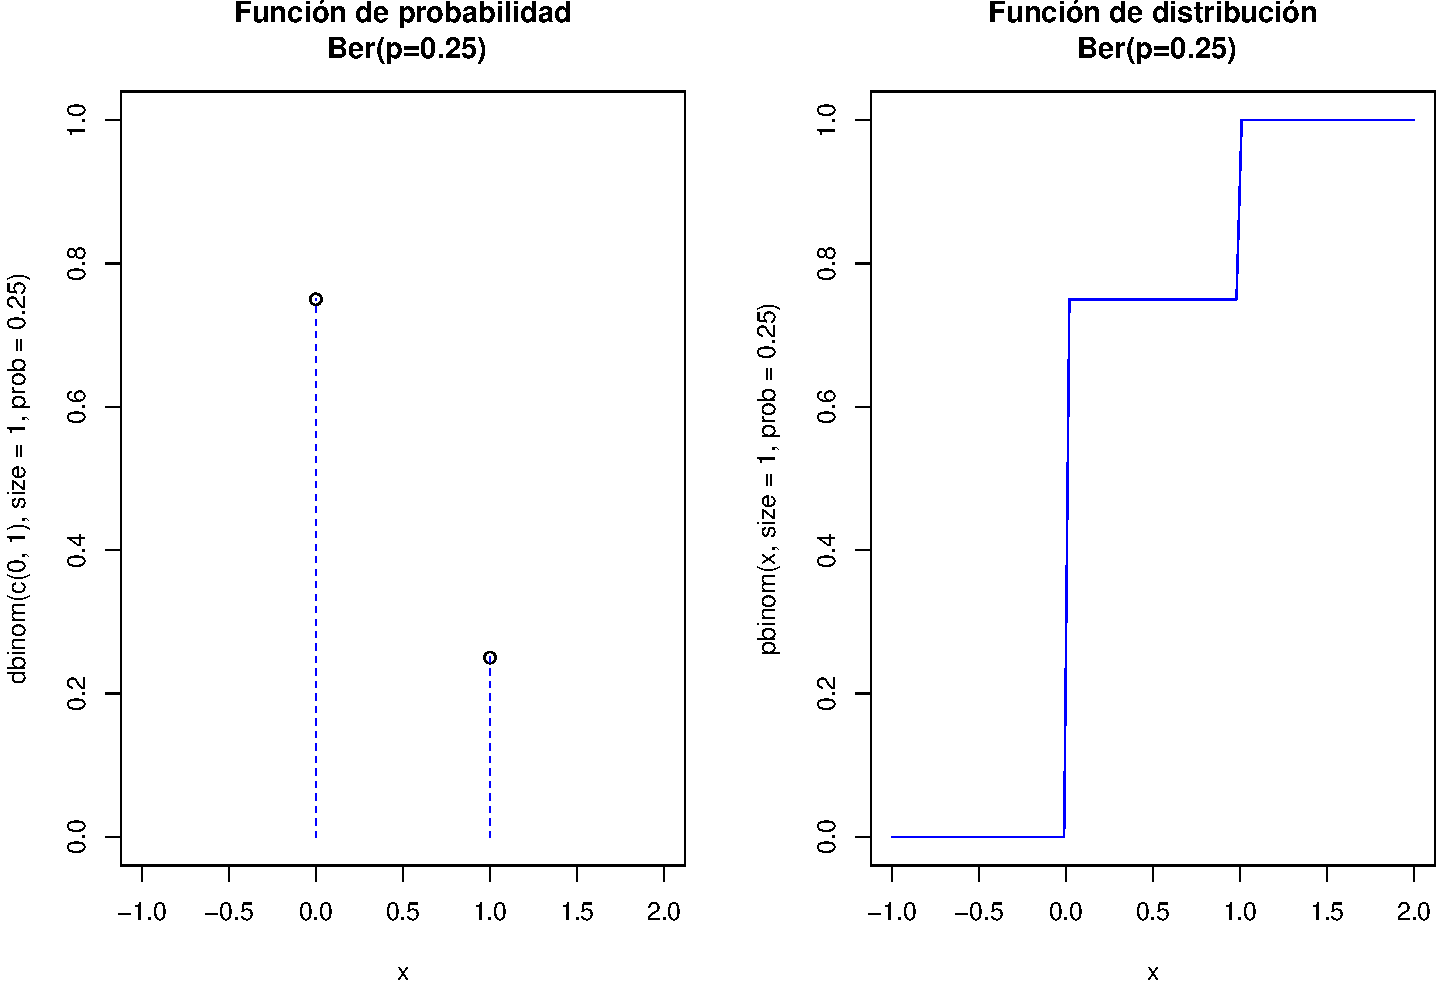
\includegraphics[width=0.7\textwidth,height=\textheight]{Tema_3_1_Notables_files/figure-beamer/ber_plot_1-1.pdf}

}

\end{figure}
\end{frame}

\hypertarget{distribuciuxf3n-binomial}{%
\section{Distribución binomial}\label{distribuciuxf3n-binomial}}

\begin{frame}{Distribución binomial}
\protect\hypertarget{distribuciuxf3n-binomial-1}{}
Distribución binomial

Si repetimos \(n\) veces de forma independiente un experimento Bernoulli
de parámetro \(p\).

El espacio muestral \(\Omega\) estará formado por cadenas de \(E\)'s y
\(F\)'s de longitud \(n\) Consideremos la v.a.

\[X(\overbrace{EFFF\ldots EEF}^{n})=\mbox{número de éxitos en la cadena}.\]
A la variable aleatoria anterior se le conoce como distribución binomial
de parámetros \(n\) y \(p\), y lo denotaremos por \(X\equiv B(n,p).\)
\end{frame}

\begin{frame}{Función de probabilidad de una binomial}
\protect\hypertarget{funciuxf3n-de-probabilidad-de-una-binomial}{}
Entonces su \textbf{función de probabilidad} es

\[
P_{X}(x)=\left\{
\begin{array}{ll}
{n\choose x}\cdot  p^x \cdot(1-p)^{n-x} &\mbox{ si } x=0,1,\ldots,n\\
0  & \mbox{ en otro caso}
\end{array}\right..
\]
\end{frame}

\begin{frame}{Función de distribución de binomial}
\protect\hypertarget{funciuxf3n-de-distribuciuxf3n-de-binomial}{}
Su \textbf{función de distribución} no tiene una fórmula cerrada. Hay
que acumular la función de probabilidad:

\begin{eqnarray*}
F_{X}(x)=P(X\leq x) & = & \sum_{i=0}^x P_X(i)\\
& = & 
\left\{
\begin{array}{ll}
0 & \mbox{ si } x<0\\\displaystyle
\sum_{i=0}^k {n\choose i}\cdot  p^i \cdot (1-p)^{n-i} & \mbox{ si } 
\left\{
  \begin{array}{l} 
  k\leq x< k+1\\
  k=0,1,\ldots,n.
  \end{array}
\right.\\
1 & \mbox{ si } n\leq x
\end{array}
\right.
\end{eqnarray*}
\end{frame}

\begin{frame}[fragile]{Números binomiales con R}
\protect\hypertarget{nuxfameros-binomiales-con-r}{}
Los números binomiales calculan el número de equipos de baloncesto
distintos que (\(k=5\) jugadores) se pueden hacer con 6 jugadores
(\(n=6\)).

Es decir cuántas maneras distintas hay para elegir (\emph{choose}) 5
jugadores en un conjunto de 6 jugadores. Todo el mundo diría ¡¡¡6!!!.
Efectivamente con R es

\begin{Shaded}
\begin{Highlighting}[]
\FunctionTok{choose}\NormalTok{(}\DecValTok{6}\NormalTok{,}\DecValTok{5}\NormalTok{)}
\end{Highlighting}
\end{Shaded}

\begin{verbatim}
[1] 6
\end{verbatim}
\end{frame}

\begin{frame}[fragile]{Números binomiales con R}
\protect\hypertarget{nuxfameros-binomiales-con-r-1}{}
Con 10 jugadores el número de equipos de 5 distintos es bastante más
grande

\begin{Shaded}
\begin{Highlighting}[]
\FunctionTok{choose}\NormalTok{(}\DecValTok{10}\NormalTok{,}\DecValTok{5}\NormalTok{)}
\end{Highlighting}
\end{Shaded}

\begin{verbatim}
[1] 252
\end{verbatim}

Y, por ejemplo, con un equipo de fútbol profesional que tiene en
plantilla 22 jugadores (quitando los guardametas) se pueden formar
¡¡nada menos que!!

\begin{Shaded}
\begin{Highlighting}[]
\FunctionTok{choose}\NormalTok{(}\DecValTok{22}\NormalTok{,}\DecValTok{10}\NormalTok{)}
\end{Highlighting}
\end{Shaded}

\begin{verbatim}
[1] 646646
\end{verbatim}

un bonito número capicúa que nos da el número de equipos distintos que
se pueden formar.
\end{frame}

\begin{frame}{Distribución Binomial}
\protect\hypertarget{distribuciuxf3n-binomial-2}{}
Obviamente se tiene que una v.a. Bernoulli es una binomial con \(n=1\)

\[B(1,p)=Ber(p).\]

\textbf{Ejercicio}

Calculad las funciones de distribución de una binomial \(B(n=1,p=0.3)\)
y comprobar que coinciden con las distribuciones de una \(Ber(p=0.3)\).
\end{frame}

\begin{frame}{Observaciones sobre la distribución binomial}
\protect\hypertarget{observaciones-sobre-la-distribuciuxf3n-binomial}{}
\begin{itemize}
\tightlist
\item
  La probabilidad de fracaso se suele denotar con \(q=1-p\), \textbf{sin
  ningún aviso adicional}, con el fin de acortar y agilizar la escritura
  de las fórmulas.
\item
  Su \textbf{función de distribución no tienen una formula general}, hay
  que calcularla con una función de R o python\ldots{} En el siglo
  pasado se tabulaban en los libros de papel :-).
\item
  En el material adicional os pondremos unas tablas de esta distribución
  para distintos valores de \(n\) y \(p\) para que disfrutéis de tan
  ancestral método de cálculo.
\item
  Cualquier paquete estadístico, hoja de cálculo dispone de funciones
  para el cálculo de estas probabilidades, así que el \textbf{uso de las
  tablas} queda \textbf{totalmente anticuado}.
\end{itemize}
\end{frame}

\begin{frame}{Esperanza de una \(B(n,p)\)}
\protect\hypertarget{esperanza-de-una-bnp}{}
Su \textbf{esperanza} es
\[E(X)=\displaystyle\sum_{k=0}^n k \cdot  {n \choose k }\cdot p^k\cdot q^{n-k} = n\cdot p.\]

La esperanza de \(X^2\) es

\begin{eqnarray*}
E(X^2)&=& \displaystyle\sum_{k=0}^n k^2 \cdot  {n \choose k }\cdot p^k\cdot q^{n-k}\\
&=& n\cdot p\cdot q+(n\cdot p)^2.
\end{eqnarray*}
\end{frame}

\begin{frame}{Varianza de una \(B(n,p)\)}
\protect\hypertarget{varianza-de-una-bnp}{}
Su \textbf{varianza} es

\[Var(X)=E(X^2)-\left(E(X)\right)^2=n\cdot p \cdot q=n\cdot p\cdot (1-p).\]

Su desviación típica es

\[\sqrt{n\cdot p\cdot q}=\sqrt{n\cdot p\cdot (1-p)}.\]

En temas posteriores veremos una forma sencilla del cálculo de la
esperanza y varianza de una \(B(n,p)\) como las suma de \(n\) v.a.
\(Ber(p)\) independientes.

\textbf{Ejercicio}

Justificar de forma intuitiva que si \(X_i\) con \(i=1,2,\ldots, n\) son
v.a. \(Ber(p)\) independientes entonces
\(X=\displaystyle\sum_{i=1}^n X_i\) sigue una distribución \(B(n,p).\)
\end{frame}

\begin{frame}{Resumen v.a con distribución binomial \(B(n,p)\)}
\protect\hypertarget{resumen-v.a-con-distribuciuxf3n-binomial-bnp}{}
\renewcommand{\arraystretch}{1.75}
\begin{table}
\centering
\begin{tabular}{|l|}
\hline\rowcolor{LightBlue}
$X$ binomial:   $B(n,p)$ \\\hline
$\scriptstyle  D_X=   \{0,1,\ldots n\}$  \\\hline
$\scriptstyle P_X(x)=P(X=x)=\left\{\begin{array}{ll}\scriptstyle {n\choose x}\cdot  p^x\cdot  (1-p)^{n-x} & \mbox{ si } x=0,1,\ldots,n\\0  & \mbox{ en otro caso.}\end{array}\right.$ \\\hline
$\scriptstyle  F_X(x)=P(X\leq X)=
\scriptstyle\left\{
\begin{array}{ll}
\scriptstyle  0 & \scriptstyle  \mbox{ si } x<0\\ 
\scriptstyle \sum_{i=0}^k {n\choose i}\cdot  p^i\cdot  (1-p)^{n-i} &  
\scriptstyle \mbox{si } \scriptstyle k\leq x< k+1 \mbox{\small para } \scriptstyle k=0,1,\dots,n \\ 
\scriptstyle 1 & \scriptstyle  \mbox{ si } x\geq n
\end{array}
\right.$.\\\hline
$\scriptstyle E(X)=n\cdot p$; $\scriptstyle  Var(X)=n\cdot p \cdot (1-p)$ \\\hline
\end{tabular}
\end{table}
\end{frame}

\begin{frame}[fragile]{Cálculos binomial con R}
\protect\hypertarget{cuxe1lculos-binomial-con-r}{}
Veamos los cálculos básicos con funciones de R para una v.a \(X\) con
distribución binomial \(B(n=10,p=0.25)\).

Si queremos calcular con \texttt{R} algún valor de la función de
distribución como por ejemplo \(F_X(0)=P(X\leq 0)\), tenemos que hacer:

\begin{Shaded}
\begin{Highlighting}[]
\FunctionTok{pbinom}\NormalTok{(}\DecValTok{0}\NormalTok{,}\AttributeTok{size=}\DecValTok{10}\NormalTok{,}\AttributeTok{prob=}\FloatTok{0.25}\NormalTok{)}
\end{Highlighting}
\end{Shaded}

\begin{verbatim}
[1] 0.05631351
\end{verbatim}

y si queremos por ejemplo \(F_X(4)=P(X\leq 4)\), tenemos que hacer:

\begin{Shaded}
\begin{Highlighting}[]
\FunctionTok{pbinom}\NormalTok{(}\DecValTok{4}\NormalTok{,}\AttributeTok{size=}\DecValTok{10}\NormalTok{,}\AttributeTok{prob=}\FloatTok{0.25}\NormalTok{)}
\end{Highlighting}
\end{Shaded}

\begin{verbatim}
[1] 0.9218731
\end{verbatim}
\end{frame}

\begin{frame}[fragile]{Cálculos binomial con R}
\protect\hypertarget{cuxe1lculos-binomial-con-r-1}{}
Sin embargo, si queremos calcular algún valor de la función de
probabilidad como por ejemplo \(P(X=0)\), tenemos que hacer:

\begin{Shaded}
\begin{Highlighting}[]
\FunctionTok{dbinom}\NormalTok{(}\DecValTok{0}\NormalTok{,}\AttributeTok{size=}\DecValTok{10}\NormalTok{,}\AttributeTok{prob=}\FloatTok{0.25}\NormalTok{)}
\end{Highlighting}
\end{Shaded}

\begin{verbatim}
[1] 0.05631351
\end{verbatim}

o por ejemplo para \(P(X=4)\):

\begin{Shaded}
\begin{Highlighting}[]
\FunctionTok{dbinom}\NormalTok{(}\DecValTok{4}\NormalTok{,}\AttributeTok{size=}\DecValTok{10}\NormalTok{,}\AttributeTok{prob=}\FloatTok{0.25}\NormalTok{)}
\end{Highlighting}
\end{Shaded}

\begin{verbatim}
[1] 0.145998
\end{verbatim}
\end{frame}

\begin{frame}[fragile]{Generación de muestras aleatorias con R}
\protect\hypertarget{generaciuxf3n-de-muestras-aleatorias-con-r}{}
Generaremos una muestra aleatoria de 100 valores de una población con
distribución \(B(20,0.5)\)

\begin{Shaded}
\begin{Highlighting}[]
\FunctionTok{set.seed}\NormalTok{(}\DecValTok{2019}\NormalTok{)}
\FunctionTok{rbinom}\NormalTok{(}\DecValTok{100}\NormalTok{,}\AttributeTok{size =} \DecValTok{20}\NormalTok{,}\AttributeTok{prob=}\FloatTok{0.5}\NormalTok{)}
\end{Highlighting}
\end{Shaded}

\begin{verbatim}
  [1] 12 11  9 11  6  6 12  5  7 11 12 11  8  8 11 11  7 11  9 10  9 10 14  8  8
 [26]  5 11 14 11 10 11  5 12  8  6  7  9 10  5 12 11  9 12 11 12 10 13 13  8  8
 [51]  9  7  6  9 10  9 16 13  6  6  8  8 11  9 12 15  9  7 12 11  9  8  9  8 11
 [76] 15  7 10  9 12  6 13 14  8 10  8 10 11 11  9 10 11 12  8 10 12  9 13  9 13
\end{verbatim}

\textbf{Ejemplo}

El ejemplo anterior correspondería a repetir 100 veces el experimento de
lanzar una moneda 20 veces y contar el número de caras.
\end{frame}

\begin{frame}[fragile]{Cálculos distribución binomial con python}
\protect\hypertarget{cuxe1lculos-distribuciuxf3n-binomial-con-python}{}
Veamos los cálculos básicos con funciones de python para una v.a \(X\)
con distribución binomial \(B(n=10,p=0.25)\).

Primero importamos la función \texttt{binom} de la librería
\texttt{scipy.stat}

\begin{Shaded}
\begin{Highlighting}[]
\ImportTok{from}\NormalTok{ scipy.stats }\ImportTok{import}\NormalTok{ binom}
\end{Highlighting}
\end{Shaded}

En general en el paquete \texttt{scipy}, la función de probabilidad se
invocará con el método \texttt{pmf}, la de distribución con el método
\texttt{cdf} mientras que una muestra aleatoria que siga esta
distribución con el método \texttt{rvs}. En todos ellos aparecerá
siempre el parámetro \texttt{loc} que se utiliza para desplazar el
dominio de la variable aleatoria. Por ejemplo, en este caso

\begin{Shaded}
\begin{Highlighting}[]
\NormalTok{binom.pmf(k, n, p, loc) }\OperatorTok{=}\NormalTok{  binom.pmf(k }\OperatorTok{{-}}\NormalTok{ loc, n, p)}
\end{Highlighting}
\end{Shaded}
\end{frame}

\begin{frame}[fragile]{Cálculos distribución binomial con python}
\protect\hypertarget{cuxe1lculos-distribuciuxf3n-binomial-con-python-1}{}
Para calcular los valores de la función de distribución como por ejemplo
\(F_X(0)=P(X\leq 0)\) y \(F_X(4)=P(X\leq 4)\) utilizamos la función
\texttt{cdf}

\begin{Shaded}
\begin{Highlighting}[]
\NormalTok{binom.cdf(}\DecValTok{0}\NormalTok{,n}\OperatorTok{=}\DecValTok{10}\NormalTok{,p}\OperatorTok{=}\FloatTok{0.25}\NormalTok{)}
\end{Highlighting}
\end{Shaded}

\begin{verbatim}
0.056313514709472684
\end{verbatim}

\begin{Shaded}
\begin{Highlighting}[]
\NormalTok{binom.cdf(}\DecValTok{4}\NormalTok{,n}\OperatorTok{=}\DecValTok{10}\NormalTok{,p}\OperatorTok{=}\FloatTok{0.25}\NormalTok{)}
\end{Highlighting}
\end{Shaded}

\begin{verbatim}
0.9218730926513672
\end{verbatim}

Notemos que al no indicar el valor de \texttt{loc}, se le asume que toma
el valor 0.
\end{frame}

\begin{frame}[fragile]{Cálculos distribución binomial con python}
\protect\hypertarget{cuxe1lculos-distribuciuxf3n-binomial-con-python-2}{}
Para calcular los valores de la función de probabilidad \(P(X=0)\) y
\(P(X=4)\) utilizamos la función \texttt{pmf}:

\begin{Shaded}
\begin{Highlighting}[]
\NormalTok{binom.pmf(}\DecValTok{0}\NormalTok{,n}\OperatorTok{=}\DecValTok{10}\NormalTok{,p}\OperatorTok{=}\FloatTok{0.25}\NormalTok{)}
\end{Highlighting}
\end{Shaded}

\begin{verbatim}
0.056313514709472656
\end{verbatim}

\begin{Shaded}
\begin{Highlighting}[]
\NormalTok{binom.pmf(}\DecValTok{4}\NormalTok{,n}\OperatorTok{=}\DecValTok{10}\NormalTok{,p}\OperatorTok{=}\FloatTok{0.25}\NormalTok{)}
\end{Highlighting}
\end{Shaded}

\begin{verbatim}
0.14599800109863284
\end{verbatim}

Notemos que al no indicar el valor de \texttt{loc}, se le asume que toma
el valor 0.
\end{frame}

\begin{frame}[fragile]{Cálculos distribución binomial con python}
\protect\hypertarget{cuxe1lculos-distribuciuxf3n-binomial-con-python-3}{}
Si queremos generar una muestras aleatorias que siga una distribución
binomial, podemos usar la función \texttt{rvs}. En este caso,
generaremos una muestra aleatoria de 100 valores de una población
\(B(20,0.5)\)

\begin{Shaded}
\begin{Highlighting}[]
\NormalTok{binom.rvs(n}\OperatorTok{=}\DecValTok{20}\NormalTok{,p}\OperatorTok{=}\FloatTok{0.25}\NormalTok{,size }\OperatorTok{=} \DecValTok{100}\NormalTok{)}
\end{Highlighting}
\end{Shaded}

\begin{verbatim}
array([ 7,  5,  6,  2,  5,  6,  6,  5,  1,  3,  6,  2,  2,  4,  6,  5,  5,
        5,  3,  3,  5,  5,  5,  2,  4,  4,  4,  7,  4, 11, 10,  7,  4,  6,
        7,  3,  1,  2,  5,  3,  2,  7,  5,  5,  5,  7,  6,  4,  5,  5,  4,
        4,  5,  5,  7,  9,  4,  4,  3,  3,  4,  4,  2,  3,  3,  7,  8,  4,
        6,  3,  7,  1,  3,  1,  9,  4,  4,  3,  5,  5,  4,  6,  7,  7,  6,
        4,  7,  7,  2,  2,  5,  9,  4,  2,  6,  6,  3,  4,  7,  2],
      dtype=int64)
\end{verbatim}
\end{frame}

\begin{frame}[fragile]{Cálculos distribución binomial con python}
\protect\hypertarget{cuxe1lculos-distribuciuxf3n-binomial-con-python-4}{}
Observación Notemos que la secuencia aleatoria generada no es la misma
que con \texttt{R}. De hecho, si volvemos a ejecutar esta función
obtendremos una muestra aleatoria distinta.

\begin{Shaded}
\begin{Highlighting}[]
\NormalTok{binom.rvs(n}\OperatorTok{=}\DecValTok{20}\NormalTok{,p}\OperatorTok{=}\FloatTok{0.25}\NormalTok{,size }\OperatorTok{=} \DecValTok{100}\NormalTok{)}
\end{Highlighting}
\end{Shaded}

\begin{verbatim}
array([ 7,  4,  8,  4,  1,  4,  4,  5,  4,  4,  1,  7,  7,  5,  6,  6,  4,
        3,  3,  4,  6, 10,  6,  6,  0,  5,  5,  3,  3,  4,  9,  6,  4,  5,
        7,  3,  8,  7,  5,  8,  5,  6,  7,  4,  5,  5,  1,  6,  4,  4,  5,
        5,  2,  6,  5,  6,  3,  2,  8,  4,  7,  4,  6,  8,  7,  6,  7,  4,
        4,  5,  3,  4,  3,  6,  0,  8,  5,  5,  5,  4,  4,  5,  6,  7,  5,
        5,  6,  6,  3,  5,  6,  6,  3,  7,  6,  6,  3,  4,  7,  5],
      dtype=int64)
\end{verbatim}
\end{frame}

\begin{frame}[fragile]{Cálculos binomial con python}
\protect\hypertarget{cuxe1lculos-binomial-con-python}{}
Veamos algunos cálculos básicos con funciones de python para la binomial
\(B(n=10,p=0.25)\).

\begin{Shaded}
\begin{Highlighting}[]
\NormalTok{binom.cdf(}\DecValTok{5}\NormalTok{,n}\OperatorTok{=}\DecValTok{10}\NormalTok{,p}\OperatorTok{=}\FloatTok{0.25}\NormalTok{)}
\end{Highlighting}
\end{Shaded}

\begin{verbatim}
0.9802722930908203
\end{verbatim}

\begin{Shaded}
\begin{Highlighting}[]
\NormalTok{binom.pmf(}\DecValTok{1}\NormalTok{,n}\OperatorTok{=}\DecValTok{10}\NormalTok{,p}\OperatorTok{=}\FloatTok{0.25}\NormalTok{)}
\end{Highlighting}
\end{Shaded}

\begin{verbatim}
0.1877117156982421
\end{verbatim}

\begin{Shaded}
\begin{Highlighting}[]
\NormalTok{binom.rvs(n}\OperatorTok{=}\DecValTok{20}\NormalTok{,p}\OperatorTok{=}\FloatTok{0.25}\NormalTok{,size}\OperatorTok{=}\DecValTok{10}\NormalTok{)}
\end{Highlighting}
\end{Shaded}

\begin{verbatim}
array([8, 5, 8, 4, 4, 4, 4, 3, 6, 3], dtype=int64)
\end{verbatim}
\end{frame}

\begin{frame}[fragile]{Gráficas de la distribución binomial con R}
\protect\hypertarget{gruxe1ficas-de-la-distribuciuxf3n-binomial-con-r}{}
El siguiente código de R dibuja las función de probabilidad y la de
distribución de una \(B(n=10,p=0.25)\)

\begin{Shaded}
\begin{Highlighting}[]
\FunctionTok{par}\NormalTok{(}\AttributeTok{mfrow=}\FunctionTok{c}\NormalTok{(}\DecValTok{1}\NormalTok{,}\DecValTok{2}\NormalTok{))}
\NormalTok{aux}\OtherTok{=}\FunctionTok{rep}\NormalTok{(}\DecValTok{0}\NormalTok{,}\DecValTok{22}\NormalTok{)}
\NormalTok{aux[}\FunctionTok{seq}\NormalTok{(}\DecValTok{2}\NormalTok{,}\DecValTok{22}\NormalTok{,}\DecValTok{2}\NormalTok{)]}\OtherTok{=}\FunctionTok{dbinom}\NormalTok{(}\FunctionTok{c}\NormalTok{(}\DecValTok{0}\SpecialCharTok{:}\DecValTok{10}\NormalTok{),}\AttributeTok{size=}\DecValTok{10}\NormalTok{,}\AttributeTok{prob=}\FloatTok{0.25}\NormalTok{)}
\FunctionTok{plot}\NormalTok{(}\AttributeTok{x=}\FunctionTok{c}\NormalTok{(}\DecValTok{0}\SpecialCharTok{:}\DecValTok{10}\NormalTok{),}\AttributeTok{y=}\FunctionTok{dbinom}\NormalTok{(}\FunctionTok{c}\NormalTok{(}\DecValTok{0}\SpecialCharTok{:}\DecValTok{10}\NormalTok{),}\AttributeTok{size=}\DecValTok{10}\NormalTok{,}\AttributeTok{prob=}\FloatTok{0.25}\NormalTok{),}
  \AttributeTok{ylim=}\FunctionTok{c}\NormalTok{(}\DecValTok{0}\NormalTok{,}\DecValTok{1}\NormalTok{),}\AttributeTok{xlim=}\FunctionTok{c}\NormalTok{(}\SpecialCharTok{{-}}\DecValTok{1}\NormalTok{,}\DecValTok{11}\NormalTok{),}\AttributeTok{xlab=}\StringTok{"x"}\NormalTok{,}
  \AttributeTok{main=}\StringTok{"Función de probabilidad}\SpecialCharTok{\textbackslash{}n}\StringTok{ B(n=10,p=0.25)"}\NormalTok{)}
\FunctionTok{lines}\NormalTok{(}\AttributeTok{x=}\FunctionTok{rep}\NormalTok{(}\DecValTok{0}\SpecialCharTok{:}\DecValTok{10}\NormalTok{,}\AttributeTok{each=}\DecValTok{2}\NormalTok{),}\AttributeTok{y=}\NormalTok{aux, }\AttributeTok{type =} \StringTok{"h"}\NormalTok{, }\AttributeTok{lty =} \DecValTok{2}\NormalTok{,}\AttributeTok{col=}\StringTok{"blue"}\NormalTok{)}
\FunctionTok{curve}\NormalTok{(}\FunctionTok{pbinom}\NormalTok{(x,}\AttributeTok{size=}\DecValTok{10}\NormalTok{,}\AttributeTok{prob=}\FloatTok{0.25}\NormalTok{),}
  \AttributeTok{xlim=}\FunctionTok{c}\NormalTok{(}\SpecialCharTok{{-}}\DecValTok{1}\NormalTok{,}\DecValTok{11}\NormalTok{),}\AttributeTok{col=}\StringTok{"blue"}\NormalTok{,}
  \AttributeTok{main=}\StringTok{"Función de distribución}\SpecialCharTok{\textbackslash{}n}\StringTok{ B(n=10,p=0.25)"}\NormalTok{)}
\FunctionTok{par}\NormalTok{(}\AttributeTok{mfrow=}\FunctionTok{c}\NormalTok{(}\DecValTok{1}\NormalTok{,}\DecValTok{1}\NormalTok{))}
\end{Highlighting}
\end{Shaded}
\end{frame}

\begin{frame}{Gráficas de la distribución binomial con R}
\protect\hypertarget{gruxe1ficas-de-la-distribuciuxf3n-binomial-con-r-1}{}
El siguiente código de R dibuja las función de probabilidad y la de
distribución de una \(B(n=10,p=0.25)\)

\begin{figure}

{\centering 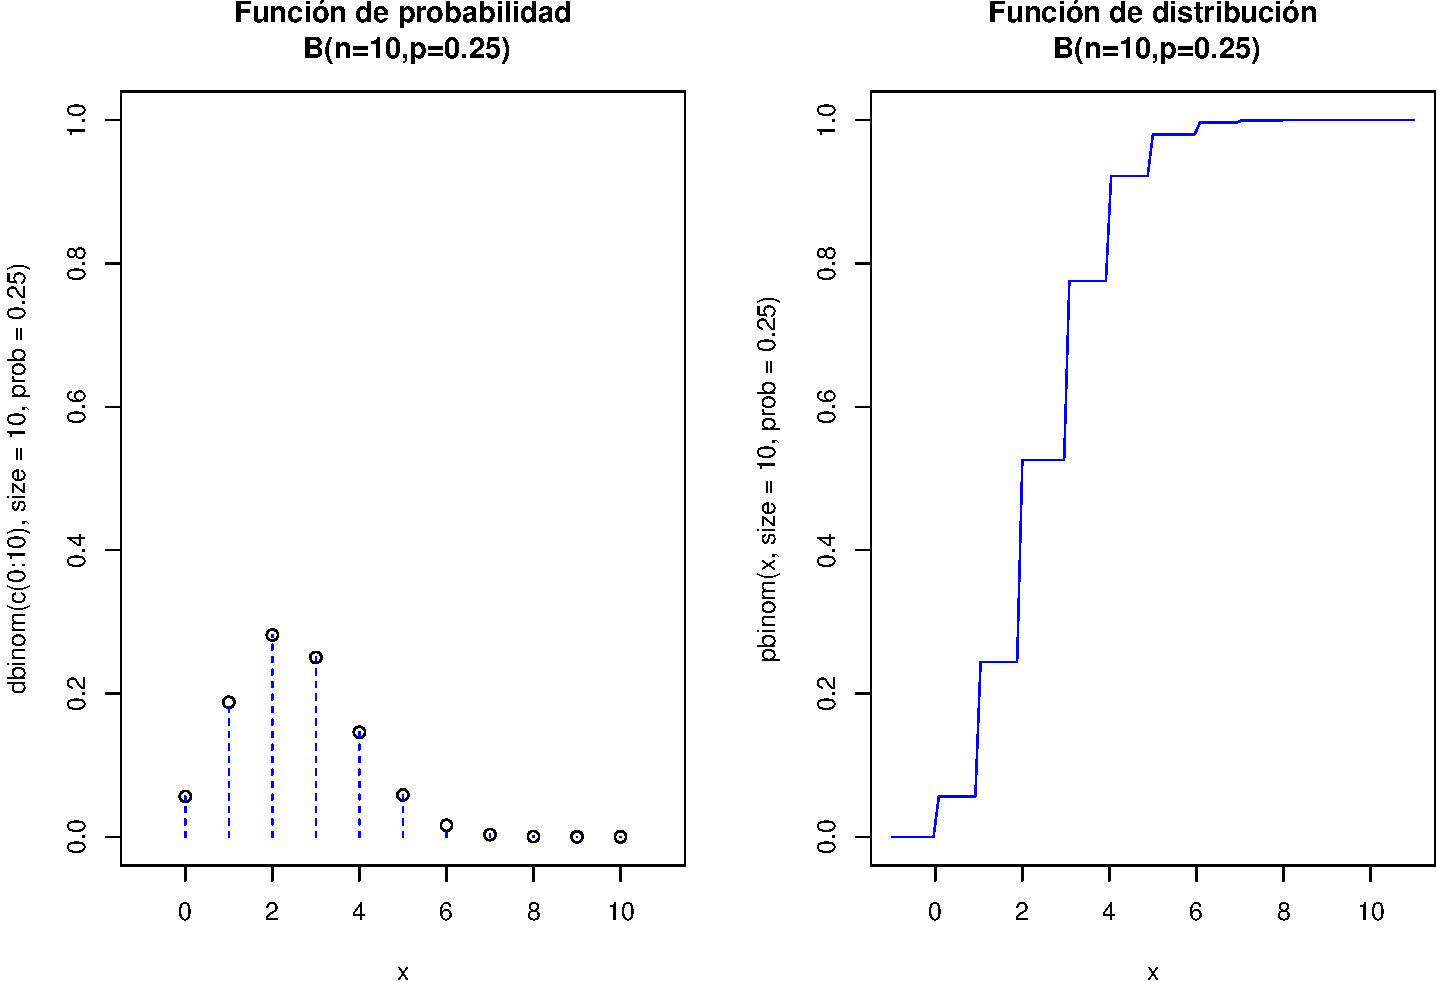
\includegraphics[width=0.55\textwidth,height=\textheight]{Tema_3_1_Notables_files/figure-beamer/unnamed-chunk-9-1.pdf}

}

\end{figure}
\end{frame}

\begin{frame}[fragile]{Gráficos de la distribución binomial con python}
\protect\hypertarget{gruxe1ficos-de-la-distribuciuxf3n-binomial-con-python}{}
\textbf{Ejercicio}

Buscad en la documentación de python cómo se dibuja la función de
probabilidad y de distribución de una binomial y recread los gráficos
anteriores.

Pista: Necesitaremos investigar más librerías:

\begin{Shaded}
\begin{Highlighting}[]
\ImportTok{import}\NormalTok{ numpy }\ImportTok{as}\NormalTok{ np}
\ImportTok{import}\NormalTok{ matplotlib.pyplot }\ImportTok{as}\NormalTok{ plt}
\end{Highlighting}
\end{Shaded}
\end{frame}

\begin{frame}[fragile]{Gráficos de la distribución binomial con python}
\protect\hypertarget{gruxe1ficos-de-la-distribuciuxf3n-binomial-con-python-1}{}
\begin{Shaded}
\begin{Highlighting}[]
\NormalTok{n, p }\OperatorTok{=} \DecValTok{10}\NormalTok{, }\FloatTok{0.25}
\NormalTok{x }\OperatorTok{=}\NormalTok{ np.arange(binom.ppf(}\FloatTok{0.01}\NormalTok{, n, p),binom.ppf(}\FloatTok{0.99}\NormalTok{, n, p))}
\NormalTok{fig }\OperatorTok{=}\NormalTok{plt.figure(figsize}\OperatorTok{=}\NormalTok{(}\DecValTok{5}\NormalTok{, }\FloatTok{2.7}\NormalTok{))}
\NormalTok{ax }\OperatorTok{=}\NormalTok{ fig.add\_subplot(}\DecValTok{1}\NormalTok{,}\DecValTok{2}\NormalTok{,}\DecValTok{1}\NormalTok{)}
\NormalTok{ax.plot(x, binom.pmf(x, n, p), }\StringTok{\textquotesingle{}bo\textquotesingle{}}\NormalTok{, ms}\OperatorTok{=}\DecValTok{8}\NormalTok{, label}\OperatorTok{=}\StringTok{\textquotesingle{}binom pmf\textquotesingle{}}\NormalTok{)}
\NormalTok{ax.vlines(x, }\DecValTok{0}\NormalTok{, binom.pmf(x, n, p), colors}\OperatorTok{=}\StringTok{\textquotesingle{}b\textquotesingle{}}\NormalTok{, lw}\OperatorTok{=}\DecValTok{5}\NormalTok{, alpha}\OperatorTok{=}\FloatTok{0.5}\NormalTok{)}
\ControlFlowTok{for}\NormalTok{ tick }\KeywordTok{in}\NormalTok{ ax.xaxis.get\_major\_ticks():}
\NormalTok{  tick.label.set\_fontsize(}\DecValTok{5}\NormalTok{)}
\ControlFlowTok{for}\NormalTok{ tick }\KeywordTok{in}\NormalTok{ ax.yaxis.get\_major\_ticks():}
\NormalTok{  tick.label.set\_fontsize(}\DecValTok{5}\NormalTok{) }
\NormalTok{ax }\OperatorTok{=}\NormalTok{ fig.add\_subplot(}\DecValTok{1}\NormalTok{,}\DecValTok{2}\NormalTok{,}\DecValTok{2}\NormalTok{)}
\NormalTok{ax.plot(x, binom.cdf(x, n, p), }\StringTok{\textquotesingle{}bo\textquotesingle{}}\NormalTok{, ms}\OperatorTok{=}\DecValTok{8}\NormalTok{, label}\OperatorTok{=}\StringTok{\textquotesingle{}binom pmf\textquotesingle{}}\NormalTok{)}
\NormalTok{ax.vlines(x, }\DecValTok{0}\NormalTok{, binom.cdf(x, n, p), colors}\OperatorTok{=}\StringTok{\textquotesingle{}b\textquotesingle{}}\NormalTok{, lw}\OperatorTok{=}\DecValTok{5}\NormalTok{, alpha}\OperatorTok{=}\FloatTok{0.5}\NormalTok{)}
\ControlFlowTok{for}\NormalTok{ tick }\KeywordTok{in}\NormalTok{ ax.xaxis.get\_major\_ticks():}
\NormalTok{  tick.label.set\_fontsize(}\DecValTok{5}\NormalTok{)}
\ControlFlowTok{for}\NormalTok{ tick }\KeywordTok{in}\NormalTok{ ax.yaxis.get\_major\_ticks():}
\NormalTok{  tick.label.set\_fontsize(}\DecValTok{5}\NormalTok{)}
\NormalTok{fig.suptitle(}\StringTok{\textquotesingle{}Distribucion Binomial\textquotesingle{}}\NormalTok{)}
\NormalTok{plt.show()}
\end{Highlighting}
\end{Shaded}
\end{frame}

\begin{frame}{Gráficos de la distribución binomial con python}
\protect\hypertarget{gruxe1ficos-de-la-distribuciuxf3n-binomial-con-python-2}{}
\begin{figure}

{\centering 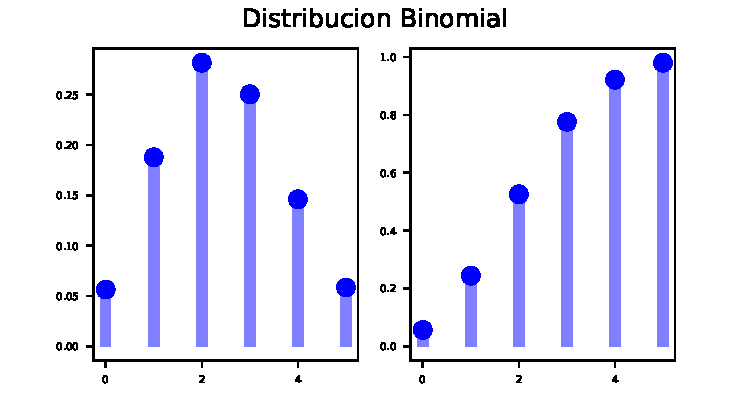
\includegraphics[width=0.7\textwidth,height=\textheight]{Tema_3_1_Notables_files/figure-beamer/dibu_python2-1.pdf}

}

\end{figure}
\end{frame}

\begin{frame}{Ejemplo distribución binomial}
\protect\hypertarget{ejemplo-distribuciuxf3n-binomial}{}
\textbf{Ejemplo: número de bolas rojas extraídas de una urna con
reposición}

Tenemos una urna con \(100\) bolas de las cuales 40 son rojas y 60 son
blancas. Extraemos al azar una bola, anotamos su color y la devolvemos a
(reponemos en) la urna.

Supongamos que repetimos este proceso \(n=10\) reponiendo en cada
ocasión la bola extraída.

Consideremos la variable aleatoria \(X\) como el número de bolas rojas
extraídas (con reposición) en \(n=10\) repeticiones del mismo
experimento de Bernoulli.

Bajo estas condiciones repetimos \(n=10\) veces el mismo experimento de
Bernoulli con probabilidad de éxito (sacar bola roja)
\[P(Roja)=P(Éxito)=p=\frac{40}{100}=0.4.\]

Así que la variable \(X\) que es el número de bolas rojas extraídas de
la urna (con reposición) en \(n=10\) ocasiones sigue una ley binomial
\(B(n=10,p=0.4).\)
\end{frame}

\begin{frame}{Ejemplo \(B(n=10,p=0.4).\)}
\protect\hypertarget{ejemplo-bn10p0.4.}{}
Nos preguntamos:

\begin{enumerate}
\tightlist
\item
  ¿Cuál es la probabilidad de que saquemos exactamente \(4\) bolas
  rojas?
\item
  ¿Cuál es la probabilidad de que saquemos al menos \(4\) bolas rojas?
\item
  ¿Cuál es la probabilidad de que saquemos menos de \(3\) bolas rojas?
\item
  ¿Cuál es el valor esperado del número de bolas rojas?
\item
  ¿Cuál es la desviación típica del número de bolas rojas?
\end{enumerate}
\end{frame}

\begin{frame}[fragile]{Ejemplo \(B(n=10,p=0.4).\)}
\protect\hypertarget{ejemplo-bn10p0.4.-1}{}
\textbf{Solución 1}. ¿Cuál es la probabilidad de que saquemos
exactamente \(4\) rojas?

Utilizando la función de probabilidad, tenemos que: \begin{eqnarray*}
P(X=4)&=&{10\choose 4}\cdot 0.4^4\cdot (1-0.4)^{10-4}
= \frac{10!}{(10-4)!\cdot 4!}\cdot 0.4^4\cdot 0.6^6\\
&=& \frac{7\cdot 8\cdot 9\cdot 10}{1\cdot 2\cdot 3\cdot 4}\cdot 0.4^4\cdot 0.6^6=0.2508227.
\end{eqnarray*}

Con R

\begin{Shaded}
\begin{Highlighting}[]
\FunctionTok{dbinom}\NormalTok{(}\DecValTok{4}\NormalTok{,}\AttributeTok{size=}\DecValTok{10}\NormalTok{,}\AttributeTok{prob =} \FloatTok{0.4}\NormalTok{)}
\end{Highlighting}
\end{Shaded}

\begin{verbatim}
[1] 0.2508227
\end{verbatim}
\end{frame}

\begin{frame}{Ejemplo \(B(n=10,p=0.4).\)}
\protect\hypertarget{ejemplo-bn10p0.4.-2}{}
\textbf{Solución 2}. ¿Cuál es la probabilidad de que saquemos al menos
\(4\) bolas rojas?

La probabilidad de sacar al menos 4 rojas se expresa como

\(P(X \geq 4)=1-P(X<4)=1-P(X\leq 3):\)

\begin{eqnarray*}
P(x\leq 3)&=& P(X=0)+P(X=1)+P(X=2)+P(X=3)\\
&=& 
 {10\choose 0}\cdot 0.4^0\cdot (1-0.4)^{10-0}+ {10\choose 1}\cdot 0.4^1\cdot (1-0.4)^{10-1}\\
&+&{10\choose 2}\cdot 0.4^2\cdot (1-0.4)^{10-2}+ {10\choose 3}\cdot 0.4^3\cdot (1-0.4)^{10-3}\\
&=&0.3822806.
\end{eqnarray*}
\end{frame}

\begin{frame}[fragile]{Ejemplo \(B(n=10,p=0.4).\)}
\protect\hypertarget{ejemplo-bn10p0.4.-3}{}
Con \texttt{R}

\begin{Shaded}
\begin{Highlighting}[]
\FunctionTok{pbinom}\NormalTok{(}\DecValTok{3}\NormalTok{,}\DecValTok{10}\NormalTok{,}\FloatTok{0.4}\NormalTok{)}
\end{Highlighting}
\end{Shaded}

\begin{verbatim}
[1] 0.3822806
\end{verbatim}

Así que

\[P(X \geq 4 )=1-P(X< 4)=1-P(X\leq 3)=1-0.3822806=0.6177194.\]
\end{frame}

\begin{frame}[fragile]{Ejemplo \(B(n=10,p=0.4).\)}
\protect\hypertarget{ejemplo-bn10p0.4.-4}{}
Otra manera usando \texttt{R} sería:

\begin{Shaded}
\begin{Highlighting}[]
\DecValTok{1}\SpecialCharTok{{-}}\FunctionTok{pbinom}\NormalTok{(}\DecValTok{3}\NormalTok{,}\DecValTok{10}\NormalTok{,}\FloatTok{0.4}\NormalTok{)}
\end{Highlighting}
\end{Shaded}

\begin{verbatim}
[1] 0.6177194
\end{verbatim}

Aunque en estos casos el parámetro \texttt{lower.tail\ =\ FALSE} es sin
duda nuestra mejor opción:

\begin{Shaded}
\begin{Highlighting}[]
\FunctionTok{pbinom}\NormalTok{(}\DecValTok{3}\NormalTok{,}\DecValTok{10}\NormalTok{,}\FloatTok{0.4}\NormalTok{,}\AttributeTok{lower.tail =} \ConstantTok{FALSE}\NormalTok{)}
\end{Highlighting}
\end{Shaded}

\begin{verbatim}
[1] 0.6177194
\end{verbatim}
\end{frame}

\begin{frame}[fragile]{Ejemplo \(B(n=10,p=0.4).\)}
\protect\hypertarget{ejemplo-bn10p0.4.-5}{}
\textbf{Solución 3}. ¿Cuál es la probabilidad de que saquemos menos de
\(3\) bolas rojas?

\begin{eqnarray*}
P(X< 3)&=& P(X\leq 2)=  P(X=0)+P(X=1)+P(X=2)\\
&=& 
{10\choose 0}\cdot 0.4^0\cdot (1-0.4)^{10-0}+ {10\choose 1}\cdot 0.4^1\cdot (1-0.4)^{10-1}\\
&&+
{10\choose 2}\cdot 0.4^2\cdot (1-0.4)^{10-2}\\
&=&0.1672898.
\end{eqnarray*}

En \texttt{R}:

\begin{Shaded}
\begin{Highlighting}[]
\FunctionTok{dbinom}\NormalTok{(}\DecValTok{0}\NormalTok{,}\DecValTok{10}\NormalTok{,}\FloatTok{0.4}\NormalTok{)}\SpecialCharTok{+}\FunctionTok{dbinom}\NormalTok{(}\DecValTok{1}\NormalTok{,}\DecValTok{10}\NormalTok{,}\FloatTok{0.4}\NormalTok{)}\SpecialCharTok{+}\FunctionTok{dbinom}\NormalTok{(}\DecValTok{2}\NormalTok{,}\DecValTok{10}\NormalTok{,}\FloatTok{0.4}\NormalTok{)}
\end{Highlighting}
\end{Shaded}

\begin{verbatim}
[1] 0.1672898
\end{verbatim}

\begin{Shaded}
\begin{Highlighting}[]
\FunctionTok{pbinom}\NormalTok{(}\DecValTok{2}\NormalTok{,}\DecValTok{10}\NormalTok{,}\FloatTok{0.4}\NormalTok{)}
\end{Highlighting}
\end{Shaded}

\begin{verbatim}
[1] 0.1672898
\end{verbatim}
\end{frame}

\begin{frame}[fragile]{Ejemplo \(B(n=10,p=0.4).\)}
\protect\hypertarget{ejemplo-bn10p0.4.-6}{}
\textbf{Solución 4}. ¿Cuál es el valor esperado del número de bolas
rojas?

Como \(X\) es una \(B(n=10,p=0.4)\) sabemos que

\[E(X)=n\cdot p = 10\cdot 0.4=4.\]

Aunque en python tenemos la función \texttt{stats} que nos lo calcula
directamente:

\begin{Shaded}
\begin{Highlighting}[]
\BuiltInTok{print}\NormalTok{(}\StringTok{"E(X) = }\SpecialCharTok{\{m\}}\StringTok{"}\NormalTok{.}\BuiltInTok{format}\NormalTok{(m}\OperatorTok{=}\NormalTok{binom.stats(n }\OperatorTok{=} \DecValTok{10}\NormalTok{, p }\OperatorTok{=} \FloatTok{0.4}\NormalTok{, moments}\OperatorTok{=}\StringTok{\textquotesingle{}m\textquotesingle{}}\NormalTok{)))}
\end{Highlighting}
\end{Shaded}

\begin{figure}

{\centering 
\includegraphics[width=0.7\textwidth,height=\textheight]{Tema_3_1_Notables_files/figure-beamer/unnamed-chunk-16-1.pdf}

}

\end{figure}
\end{frame}

\begin{frame}[fragile]{Ejemplo \(B(n=10,p=0.4).\)}
\protect\hypertarget{ejemplo-bn10p0.4.-7}{}
\textbf{Solución 5}. ¿Cuál es la desviación típica del número de bolas
rojas?

La varianza es: \[
Var(X)=n\cdot p \cdot(1-p)=10\cdot 0.4\cdot 0.6=2.4.
\]

Por lo tanto la desviación típica es

\[\sqrt{Var(X)}=\sqrt{2.4}= 1.5491933.\]

Aunque en python tenemos la función \texttt{stats} que nos lo calcula
directamente:

\begin{Shaded}
\begin{Highlighting}[]
\BuiltInTok{print}\NormalTok{(}\StringTok{"Var(X) = }\SpecialCharTok{\{v\}}\StringTok{"}\NormalTok{.}\BuiltInTok{format}\NormalTok{(v}\OperatorTok{=}\NormalTok{binom.stats(n }\OperatorTok{=} \DecValTok{10}\NormalTok{, p }\OperatorTok{=} \FloatTok{0.4}\NormalTok{, moments}\OperatorTok{=}\StringTok{\textquotesingle{}v\textquotesingle{}}\NormalTok{)))}
\end{Highlighting}
\end{Shaded}

\begin{figure}

{\centering 
\includegraphics[width=0.7\textwidth,height=\textheight]{Tema_3_1_Notables_files/figure-beamer/unnamed-chunk-17-3.pdf}

}

\end{figure}
\end{frame}

\hypertarget{distribuciuxf3n-geomuxe9trica}{%
\section{Distribución geométrica}\label{distribuciuxf3n-geomuxe9trica}}

\begin{frame}{Distribución geométrica}
\protect\hypertarget{distribuciuxf3n-geomuxe9trica-1}{}
\begin{itemize}
\item
  Todos hemos jugado a, por ejemplo, tirar una moneda hasta que
  obtengamos la primera cara.
\item
  O también tirar una pelota a una canasta de baloncesto hasta obtener
  la primera canasta.
\item
  Desde otro punto de vista también podemos intentar modelar el número
  de veces que accionamos una interruptor y la bombilla se ilumina hasta
  que falla.
\item
  O también el número de veces que un cajero automático nos da dinero
  hasta que falla.
\end{itemize}

La \textbf{modelización de este tipo de problemas se consigue con la
llamada distribución geométrica}.
\end{frame}

\begin{frame}{Distribución geométrica}
\protect\hypertarget{distribuciuxf3n-geomuxe9trica-2}{}
Distribución geométrica

\begin{itemize}
\tightlist
\item
  Repitamos un experimento Bernoulli, de parámetro \(p\), de forma
  independiente hasta obtener el primer éxito.
\item
  Sea \(X\) la v.a. que cuenta el número de fracasos antes del primer
  éxito. Por ejemplo que hayamos tenido \(x\) fracasos será una cadena
  de \(x\) fracasos culminada con un éxito. Más concretamente
\end{itemize}

\[P(\overbrace{FFF\ldots F}^{x}E)=P(F)^{x}\cdot P(E)=(1-p)^{x}\cdot p=q^{x}\cdot p.\]
\end{frame}

\begin{frame}{Distribución geométrica}
\protect\hypertarget{distribuciuxf3n-geomuxe9trica-3}{}
Su función de probabilidad es

\[
P_X(x)=P(X=x)=\left\{\begin{array}{ll}
(1-p)^{x}\cdot p & \mbox{ si } x=0,1,2,\ldots\\
0 &\mbox{ en otro caso}
\end{array}\right..
\]

\begin{itemize}
\tightlist
\item
  La v.a. definida anteriormente diremos que sigue una distribución
  geométrica de parámetro \(p\).
\item
  La denotaremos por \(Ge(p)\).
\item
  Su dominio es \(D_X=\{0,1,2,\ldots\}\).
\end{itemize}
\end{frame}

\begin{frame}{Función de distribución geométrica}
\protect\hypertarget{funciuxf3n-de-distribuciuxf3n-geomuxe9trica}{}
Calculemos P(\(X\leq 3\)).

Por la propiedad de la probabilidad del suceso complementario tenemos
que

\[
P(X\leq 3 )=1-P(X> 3)=1-P(X\geq 4)
\]

Efectivamente, el complementario del evento \(X\leq 3\) nos dice que
hemos fracasado más de tres veces hasta conseguir el primer éxito, es
decir, \textbf{hemos fracasado 4 o más veces}. Podemos simbolizar dicho
evento de la forma siguiente: \[
\{X>3\}=\{X\geq 4\}= \{FFFF\}
\]
\end{frame}

\begin{frame}{Función de distribución geométrica}
\protect\hypertarget{funciuxf3n-de-distribuciuxf3n-geomuxe9trica-1}{}
Ahora, al ser los intentos independientes, tenemos que:

\begin{eqnarray*}
P(X>3) & = & P(\{FFFF\})= P(F)\cdot P(F)\cdot P(F)\cdot P(F)\\
&=& (1-p)\cdot (1-p)\cdot (1-p)\cdot (1-p)= (1-p)^{3+1}\\
&=&(1-p)^{4}.
\end{eqnarray*}

El valor de la función de distribución de \(X\) en \(x=3\) será, pues:
\[F_X(3)=P(X\leq 3)=1-P(X>3)=1-(1-p)^{3+1}.\] Generalizando el resultado
anterior a cualquier entero positivo \(k=0,1,2,\ldots\), tenemos:
\[F_X(k)=P(X\leq k)=1-(1-p)^{k+1},\mbox{ si } k=0,1,2,\ldots\]
\end{frame}

\begin{frame}{Función de distribución geométrica}
\protect\hypertarget{funciuxf3n-de-distribuciuxf3n-geomuxe9trica-2}{}
En general, tendremos que: \[
F_X(x)=P(X\leq x)=
\left\{\begin{array}{ll} 
0, & \mbox{ si } x<0,\\
1- (1-p),  & \mbox{ si } k=0\leq x <1,\\
1- (1-p)^2, & \mbox{ si } k=1\leq x <2,\\
1- (1-p)^3, & \mbox{ si } k=2\leq x <3,\\
1- (1-p)^{k+1}, & \mbox{ si } \left\{ \begin{array}{l}k\leq x< k+1,\\\mbox{para } k=0,1,2,\ldots\end{array}
    \right.
\end{array}
\right..
\]
\end{frame}

\begin{frame}{Función de distribución geométrica}
\protect\hypertarget{funciuxf3n-de-distribuciuxf3n-geomuxe9trica-3}{}
De forma más compacta, tendremos que \[
F_X(x)=P(X\leq x)=
\left\{\begin{array}{ll} 
0, & \mbox{ si } x<0,\\
1- (1-p)^{k+1}, & \mbox{ si } \left\{ \begin{array}{l}k\leq x< k+1,\\\mbox{para } k=0,1,2,\ldots\end{array}
\right.
\end{array}
\right..
\]

Notemos que el límite de la función de distribución es: \[
\displaystyle\lim_{k\to +\infty } F_X(k)=\lim_{k\to +\infty } 1-(1-p)^{k+1}=
1,
\] ya que \(0<1-p<1\).
\end{frame}

\begin{frame}{Sumas derivadas series geométricas}
\protect\hypertarget{sumas-derivadas-series-geomuxe9tricas}{}
Recordemos del tema de variables aleatorias que

Propiedades

\begin{itemize}
\tightlist
\item
  Si \(|r|<1\) también son convergentes las derivadas, respecto de
  \(r\), de la serie geométrica y convergen a la derivada
  correspondiente. Así tenemos que
\end{itemize}

\[
\begin{array}{rlrl}
\left(\sum_{k=0}^{+\infty} r^k\right)'&= \sum_{k=1}^{+\infty}k\cdot
r^{k-1} &= \left(\frac1{1-r}\right)'=\frac1{(1-r)^2}\\
\left(\sum_{k=0}^{+\infty} r^k\right)^{''}&= \sum_{k=2}^{+\infty}k \cdot(k-1)\cdot
r^{k-2}&=\left(\frac1{1-r}\right)^{''}=\frac2{(1-r)^3}
\end{array}
\]
\end{frame}

\begin{frame}{Esperanza de una v.a. \(Ge(p)\)}
\protect\hypertarget{esperanza-de-una-v.a.-gep}{}
Recordemos que \(P(X=x)=(1-p)^x\cdot p\) si \(x=0,1,2,\ldots\) y
aplicado la fórmula anterior con \(r=1-p\)

\begin{eqnarray*}
E(X)&=&\sum_{x=0}^{+\infty} x\cdot P_x(x)=\sum_{x=0}^{+\infty} x\cdot (1-p)^x\cdot p\\
&=& p\cdot (1-p) \cdot \sum_{x=1}^{+\infty} x\cdot (1-p)^{x-1}\\
&=& p\cdot (1-p)\cdot \frac{1}{(1-(1-p))^2}=p\cdot (1-p)\cdot \frac{1}{p^2}=\frac{1-p}{p}
\end{eqnarray*}
\end{frame}

\begin{frame}{Valor \(E(X^2)\) de una v.a. \(Ge(p)\)}
\protect\hypertarget{valor-ex2-de-una-v.a.-gep}{}
\begin{eqnarray*}
E(X^2)&=&\sum_{x=0}^{+\infty} x^2\cdot P_X(x)=\sum_{x=1}^{+\infty} x^2\cdot (1-p)^x\cdot p\\
&=& 
\sum_{x=1}^{+\infty} (x\cdot (x-1)+x)\cdot (1-p)^{x}\cdot p\\
&=&
\sum_{x=1}^{+\infty} x\cdot (x-1)\cdot (1-p)^{x}\cdot p+\sum_{x=1}^{+\infty} x \cdot (1-p)^{x}\cdot p\\
&=&
(1-p)^{2}\cdot p\cdot \sum_{x=2}^{+\infty} x\cdot (x-1)\cdot (1-p)^{x-2}\\ 
&  +&   (1-p)\cdot p\sum_{x=1}^{+\infty} x \cdot (1-p)^{x-1} = \ldots
\end{eqnarray*}.
\end{frame}

\begin{frame}{Valor \(E(X^2)\) de una v.a. \(Ge(p)\)}
\protect\hypertarget{valor-ex2-de-una-v.a.-gep-1}{}
\begin{eqnarray*}
E(X^2)&=&\ldots\\
&=&
(1-p)^{2}\cdot p\cdot \sum_{x=2}^{+\infty} x\cdot (x-1)\cdot (1-p)^{x-2}\\ 
&  +&   (1-p)\cdot p\sum_{x=1}^{+\infty} x \cdot (1-p)^{x-1}\\
&=&
p\cdot (1-p)^2 \frac{2}{(1-(1-p))^3}+  (1-p)\cdot p \frac{1}{(1-(1-p))^2}\\
&=&
p\cdot (1-p)^2 \frac{2}{p^3}+  (1-p)\cdot p \frac{1}{p^2}\\
&=&\frac{2\cdot (1-p)^2}{p^2}+\frac{1-p}{p}.
\end{eqnarray*}
\end{frame}

\begin{frame}{Varianza de una v.a. \(Ge(p)\)}
\protect\hypertarget{varianza-de-una-v.a.-gep}{}
\begin{eqnarray*}
Var(X)&=&E(X^2)-E(X)^2=\frac{2\cdot (1-p)^2}{p^2}+\frac{1-p}{p}-\left(\frac{1-p}{p}\right)^2\\
&=&
\frac{2\cdot (1-p)^2+p\cdot(1-p)-(1-p)^2}{p^2}=\frac{(1-p)^2+p\cdot(1-p)}{p^2}\\
&=&
\frac{1-2\cdot p + p^2+p-p^2}{p^2}\\
&=& \frac{1-p}{p^2}.
\end{eqnarray*}

Y su desviación típica será

\[\sqrt{Var(X)}=\sqrt{\frac{1-p}{p^2}}.\]
\end{frame}

\begin{frame}{Resumen distribución geométrica \(Ge(p)\) empezando en 0}
\protect\hypertarget{resumen-distribuciuxf3n-geomuxe9trica-gep-empezando-en-0}{}
\renewcommand{\arraystretch}{1.75}
\begin{table}
\centering
\begin{tabular}{|l|}
\hline\rowcolor{LightBlue}
$X=$ Geométrica (empieza en $0$) número de fracasos  para conseguir el primer éxito
\\\hline
$D_X=\{0,1,\ldots n,\ldots\}$ \\\hline
$P_X(x)=P(X=x)=\left\{\begin{array}{ll}(1-p)^{x}\cdot p & \mbox{ si } x=0,1,2,\ldots \\0  & \mbox{ en otro caso.}\end{array}\right.$\\\hline
$F_X(x)=P(X\leq X)=\left\{\begin{array}{ll} 0 & \mbox{ si } x<0\\
  1- (1-p)^{k+1} & \mbox{ si } \left\{ \begin{array}{l}k\leq x< k+1\\\mbox{para } k=0,1,2,\ldots\end{array}
    \right.\end{array}\right.$ \\\hline
$E(X)=\frac{1-p}{p}$; $Var(X)=\frac{1-p}{p^2}$\\\hline
\end{tabular}
\end{table}
\end{frame}

\begin{frame}{La variable geométrica que cuenta los intentos para
obtener el primer éxito.}
\protect\hypertarget{la-variable-geomuxe9trica-que-cuenta-los-intentos-para-obtener-el-primer-uxe9xito.}{}
\begin{itemize}
\tightlist
\item
  Supongamos que sólo estamos interesados en el \textbf{número de
  intentos} para obtener el primer éxito.
\item
  Si definimos \(Y\)= número de intentos para obtener el primer éxito.
  Entonces \(Y=X+1\) donde \(X\equiv Ge(p)\).
\item
  Su dominio es \(D_Y=\{1,2,\ldots\}\)
\item
  La media se incrementa en un intento debido al éxito
  \(E(Y)=E(X+1)=E(X)+1=\frac{1-p}{p}+1=\frac1{p}\).
\item
  La varianza es la misma \(Var(Y)=Var(X+1)=Var(X)=\frac{1-p}{p^2}\).
\end{itemize}
\end{frame}

\begin{frame}{Resumen distribución geométrica \(Ge(p)\) empezando en
\(1\).}
\protect\hypertarget{resumen-distribuciuxf3n-geomuxe9trica-gep-empezando-en-1.}{}
\renewcommand{\arraystretch}{1.75}
\begin{table}
\centering
\begin{tabular}{|l|}
\hline\rowcolor{LightBlue}
$Y$ geométrica (que cuenta el éxito) número de \blue{INTENTOS}  para OBTENER el primer éxito
\\\hline
$D_Y=\{1,2,\ldots n,\ldots\}$ \\\hline
$P_Y(y)=P(Y=y)=\left\{\begin{array}{ll}(1-p)^{y-1}\cdot p & \mbox{ si } y=1,2,3,\ldots\\  0  & \mbox{ en otro caso.}\end{array}\right.$\\\hline
$F_Y(y)=P(Y\leq y)=\left\{\begin{array}{ll} 0 & \mbox{ si } y<1\\ 1- (1-p)^{k} & \mbox{ si } \left\{ \begin{array}{l}k\leq y< k+1\\\mbox{para } k=1,2,3,\dots \end{array}    \right.\end{array}\right.$ \\\hline
$E(X)=\frac1{p}; Var(X)=\frac{1-p}{p^2}$
\\\hline
\end{tabular}
\end{table}
\end{frame}

\begin{frame}{Propiedad de la falta de memoria}
\protect\hypertarget{propiedad-de-la-falta-de-memoria}{}
Propiedad de la falta de memoria

Sea \(X\) una v.a. discreta con dominio \(D_X=\{0,1,2,\ldots\}\), con
\(P(X=0)=p\).

Entonces \(X\) sigue una ley \(Ge(p)\) si, y sólo si, \[
P\left(X> k+j\big| X\geq j\right)=P(X> k)
\] para todo \(k,j=0,1,2,3\ldots\).
\end{frame}

\begin{frame}{Propiedad de la falta de memoria}
\protect\hypertarget{propiedad-de-la-falta-de-memoria-1}{}
\textbf{Demostración}

Si \(X\) es geométrica entonces el lado derecho de la igualdad es

\[
P(X>k)=1-P(X\leq k)=1-\left(1-(1-p)^{k+1}\right)=(1-p)^{k+1},
\] y el lado de izquierdo es

\scriptsize\{ \begin{eqnarray*}
P\left(X> k+j\big| X\geq j\right)&=&\frac{P\left(\{X> k+j\}\cap \{X\geq j\} \right)}{P\left(X\geq j\right)}=
\frac{P\left(X>k+j \right)}{P\left(X\geq j \right)} = \frac{1-P(X\leq k+j)}{1-P(X\leq j-1)}\\
&=&  \frac{1-(1-(1-p)^{k+j+1})}{1-(1-(1-p)^{j-1+1})} =\frac{(1-p)^{k+j+1}}{(1-p)^{j}} = (1-p)^{k+1},
\end{eqnarray*} \} \normalsize

lo que demuestra la igualdad.
\end{frame}

\begin{frame}{Propiedad de la falta de memoria}
\protect\hypertarget{propiedad-de-la-falta-de-memoria-2}{}
Para demostrar el recíproco, tomemos \(j=1\) y \(k\geq 0\). Entonces,
por la propiedad de la pérdida de memoria: \[
P\left(X> k+1\big| X\geq 1\right)=P(X> k)
\] Como \(P(X=0)=p\), tenemos que
\(P(X \geq 1 )=1-P(X<1)=1-P(X=0)=1-p\).

Combinado las igualdades, tenemos que:

\[
P\left(X> k+1\big| X\geq 1\right)=\frac{P(X>k+1, X\geq 1)}{P(X\geq 1)}=\frac{P(X>k+1)}{P(X\geq 1)}=P(X>k).
\] Así podemos poner que

\begin{eqnarray*}
P(X>k+1)&=&P(X\geq 1)\cdot P(X>k)=\left(1-P(X<1)\right)\cdot P(X>k)\\
&=&\left(1-P(X=0)\right)\cdot P(X>k)=(1-p)\cdot P(X>k).
\end{eqnarray*}
\end{frame}

\begin{frame}{Propiedad de la falta de memoria}
\protect\hypertarget{propiedad-de-la-falta-de-memoria-3}{}
Es decir en general tenemos que

\[
P(X>k+1)=(1-p)\cdot P(X>k)
\] Del mismo modo para \(j=2\)

\[
P(X>k+2)=(1-p)\cdot P(X>k+1)
\]

Restando la primera igualdad de la última obtenemos.

\[
P(X>k+1)-P(X>k+2)=(1-p)\cdot P(X>k)-(1-p)\cdot P(X>k+1)
\]

de donde operando en cada lado de la igualdad obtenemos la recurrencia

\[
\scriptsize{[1-P(X\leq k+1)]-[1-P(X\leq k+2)]=(1-p)\cdot [P(X>k)-P(X>k+1)]}
\] \#\# Propiedad de la falta de memoria

Ahora operando \[
P(X\leq k+2)-P(X\leq k+1)=(1-p)\cdot[1-P(X\leq k)-\left(1-P(X\leq k+1)\right)]
\] \[
P(X=k+2)=(1-p)\cdot[P(X\leq k+1)-P(X\leq k)]
\] \[
P(X=k+2)=(1-p)\cdot P(X=k+1)
\]
\end{frame}

\begin{frame}{Propiedad de la falta de memoria}
\protect\hypertarget{propiedad-de-la-falta-de-memoria-4}{}
De forma similar obtenemos

\[
P(X=k+1)=(1-p)\cdot P(X=k)
\] Utilizando la recurrencia anterior, podemos calcular todas las
probabilidades \(P(X=k)\) a partir de la \(P(X=0)=p\): \[
\scriptsize{
\begin{array}{rl}
P(X=0)&= p,\\
P(X=1)&=P(X=0+1)= (1-p)\cdot P(X=0) =(1-p)\cdot  p,\\
P(X=2)&=P(X=1+1)= (1-p)\cdot P(X=1)=(1-p)\cdot (1-p)\cdot p=(1-p)^2\cdot p,\\
 \vdots &    \vdots \\
P(X=k)&=P(X=(k-1)+1)= (1-p)\cdot P(X=k-1)=(1-p)\cdot (1-p)^{k-1}\cdot p=(1-p)^{k}\cdot p,
\end{array}
}
\] lo que demuestra el recíproco, es decir, que \(X\) es \(Geom(p)\).
\end{frame}

\begin{frame}{Falta de memoria}
\protect\hypertarget{falta-de-memoria}{}
Observación: Interpretación de la propiedad

La propiedad de la falta de memoria \[
P(X> k+j\big|X \geq j)=P(X > k),
\]\\
significa que, aunque \textbf{ya llevemos al menos \(j\) fracasos}, la
probabilidad de \textbf{que fracasemos \(k\) veces más} no disminuye, es
la misma que era cuando empezamos el experimento.

A este efecto se le suele etiquetar con la frase \textbf{el experimento
carece de memoria} o es un \textbf{experimento sin memoria}
(\emph{Memoryless Property}).
\end{frame}

\begin{frame}{Ejemplo falta de memoria}
\protect\hypertarget{ejemplo-falta-de-memoria}{}
Un ejemplo muy sencillo nos aclarará el alcance de esta propiedad

\textbf{Ejercicio: la llave que abre la puerta}

Tenemos un llavero con 10 llaves, solo una de ellas abre una puerta.
Cada vez que probamos una llave y falla olvidamos que llave hemos
probado. ¿Cuál es la probabilidad de que si ya lo hemos intentado 5
veces necesitemos más de 4 intentos adicionales para abrir la puerta?

Tomemos \(k=4,j=5\), aplicando la propiedad de la falta de memoria

\[
P(X> 4+5/X \geq 5)=P(X > 4)
\]

Después de 5 fracasos no estamos ``más cerca'' de abrir la puerta. La
propiedad de la falta de memoria nos dice que en \textbf{después de cada
intento es como si empezásemos de nuevo a abrir la puerta}. Tras 5
fracasos la probabilidad de que fallemos más de 4 veces más es la misma
que cuando lo intentamos la primera vez.
\end{frame}

\begin{frame}{Ejemplo falta de memoria}
\protect\hypertarget{ejemplo-falta-de-memoria-1}{}
¿Cuál es el número esperado de fracasos hasta abrir la puerta?

\[
E(X)=\frac{1-p}{p}=\frac{1-\frac{1}{10}}{\frac{1}{10}}=\frac{\frac{9}{10}}{\frac{1}{10}}=9.
\]

La varianza es

\[
Var(X)=\frac{1-p}{p^2}=\frac{1-\frac{1}{10}}{\left(\frac{1}{10}\right)^2}=\frac{\frac{9}{10}}{\frac{1}{100}}=
90.
\]

La desviación típica es \(\sqrt{90}=9.486833.\)
\end{frame}

\begin{frame}{Ejemplo: El clásico del fútbol}
\protect\hypertarget{ejemplo-el-cluxe1sico-del-fuxfatbol}{}
\textbf{Ejemplo: partidos hasta que el Barça gana al Madrid}

Los partidos Real Madrid vs FC Barcelona de \textbf{la liga} española se
suelen denominar \textbf{El Clásico}, sean en el Bernabeu (estadio del
Real Madrid) o en el Camp Nou (estadio del Barça)

Sea \(X\) la variable que cuenta el número de veces consecutivas que en
un partido de fútbol de la liga el Barça no gana al Madrid sea en el
Camp Nou o el Bernabeu.

Nuestra amiga Aina es muy culé (hincha del Barça) y quiere averiguar
cuántos partidos consecutivos de \textbf{El Clásico} tiene que ver hasta
ver ganar al Barça por primera vez.

Le interesa estimar cuánto le va a costar este capricho. Tendrá que
comprar las entradas y pagar los viajes de Barcelona a Madrid.

En \href{https://es.wikipedia.org/wiki/El_Cl\%C3\%A1sico}{datos
historicos de \textbf{El clásico} en la wikipedia} están los datos hasta
el 3 de marzo de 2019: se han jugado en total 178 \textbf{Clásicos}
donde el Real Madrid ganó en 72 ocasiones, el Barça, en 72 y empataron
34 veces.
\end{frame}

\begin{frame}{Ejemplo: El clásico del fútbol}
\protect\hypertarget{ejemplo-el-cluxe1sico-del-fuxfatbol-1}{}
Nos hacemos las siguientes preguntas:

\begin{itemize}
\tightlist
\item
  Si Aina solo tiene dinero para ir a ver 3 partidos, ¿cuál es la
  probabilidad de no ver ganar al Barça en al menos tres partidos
  consecutivos?
\item
  ¿Cuántos partidos se tienen que jugar de media para ver ganar al Barça
  por primera vez?
\end{itemize}

Con los datos anteriores, podemos estimar que la probabilidad de que el
Barça gane un clásico cualquiera es:

\[P(\mbox{Barça})=\frac{72}{178}=0.4045.\]

Por tanto, podemos modelar la variable \(X\), que cuenta el número de
veces consecutivas que en un partido de fútbol de la liga el Barça no
gana al Madrid, con una ley geométrica empezando en cero con
probabilidad de éxito \(p=P(\mbox{Barça})=\frac{72}{178}\),
\end{frame}

\begin{frame}{Ejemplo: El clásico del fútbol}
\protect\hypertarget{ejemplo-el-cluxe1sico-del-fuxfatbol-2}{}
\[X=Ge\left(p=\frac{72}{178}=0.4045\right)\]

Así que lo que nos pregunta Aina es la siguiente probabilidad

\[P(X\geq 3)=1-P(X\leq 2)=1-\left(1-\frac{72}{178}\right)^{2+1}=0.7888.\]

Así que Aina tiene una probabilidad del \(78.88\%\) de no ver ganar al
Barça en al menos 3 partidos antes de ver uno en el sí que gane.
\end{frame}

\begin{frame}{Variable geométrica: El clásico}
\protect\hypertarget{variable-geomuxe9trica-el-cluxe1sico}{}
Para responder a la segunda pregunta, usando que la distribución de
\(X\) es:

\[X=Ge\left(p=\frac{72}{178}=0.4045\right)\]

entonces

\[E(X)=\frac{1-p}{p}=\frac{1-0.4045}{0.4045}=1.4722\]

y

\[Var(X)=\frac{1-p}{p^2}=\frac{1-0.4045}{0.4045^2}=3.6397\]

La desviación típica es \[\sqrt{3.6397}=1.9078.\]
\end{frame}

\begin{frame}[fragile]{Cálculos con R}
\protect\hypertarget{cuxe1lculos-con-r}{}
Veamos los cálculos básicos con R para la distribución geométrica
\(Ge(p=0.25)\). R implementa la geométrica que cuenta el número de
fracasos.

\(P(X=0)=(1-0.25)^0\cdot 0.25^1=0.25\)

\begin{Shaded}
\begin{Highlighting}[]
\FunctionTok{dgeom}\NormalTok{(}\DecValTok{0}\NormalTok{,}\AttributeTok{prob=}\FloatTok{0.25}\NormalTok{)}
\end{Highlighting}
\end{Shaded}

\begin{verbatim}
[1] 0.25
\end{verbatim}

\(P(X\leq 0)=1- (1-0.25)^{0+1}=1-0.75=0.25\)

\begin{Shaded}
\begin{Highlighting}[]
\FunctionTok{pgeom}\NormalTok{(}\DecValTok{0}\NormalTok{,}\AttributeTok{prob=}\FloatTok{0.25}\NormalTok{)}
\end{Highlighting}
\end{Shaded}

\begin{verbatim}
[1] 0.25
\end{verbatim}
\end{frame}

\begin{frame}[fragile]{Cálculos con R}
\protect\hypertarget{cuxe1lculos-con-r-1}{}
\(P(X\leq 4)=1-(1-0.25)^{4+1}=1-0.75=1-0.75^5=0.7626953.\)

\begin{Shaded}
\begin{Highlighting}[]
\FunctionTok{pgeom}\NormalTok{(}\DecValTok{4}\NormalTok{,}\AttributeTok{prob=}\FloatTok{0.25}\NormalTok{)}
\end{Highlighting}
\end{Shaded}

\begin{verbatim}
[1] 0.7626953
\end{verbatim}

Una muestra aleatoria de tamaño 25 de una \(Ge(0.25)\)

\begin{Shaded}
\begin{Highlighting}[]
\FunctionTok{rgeom}\NormalTok{(}\AttributeTok{n=}\DecValTok{25}\NormalTok{,}\AttributeTok{prob=}\FloatTok{0.25}\NormalTok{)}
\end{Highlighting}
\end{Shaded}

\begin{verbatim}
 [1]  5  4  1  6 10  0  0 10  7  0  6  2  1  3  0  2  5  0  0  5  5  3  3  2  2
\end{verbatim}
\end{frame}

\begin{frame}[fragile]{Gráficos con R el código}
\protect\hypertarget{gruxe1ficos-con-r-el-cuxf3digo}{}
\begin{Shaded}
\begin{Highlighting}[]
\FunctionTok{par}\NormalTok{(}\AttributeTok{mfrow=}\FunctionTok{c}\NormalTok{(}\DecValTok{1}\NormalTok{,}\DecValTok{2}\NormalTok{))}
\NormalTok{x}\OtherTok{=}\FunctionTok{c}\NormalTok{(}\DecValTok{0}\SpecialCharTok{:}\DecValTok{10}\NormalTok{)}
\FunctionTok{plot}\NormalTok{(}\AttributeTok{x=}\NormalTok{x,}\AttributeTok{y=}\FunctionTok{dgeom}\NormalTok{(x,}\AttributeTok{prob=}\FloatTok{0.25}\NormalTok{),}
  \AttributeTok{ylim=}\FunctionTok{c}\NormalTok{(}\DecValTok{0}\NormalTok{,}\DecValTok{1}\NormalTok{),}\AttributeTok{xlim=}\FunctionTok{c}\NormalTok{(}\SpecialCharTok{{-}}\DecValTok{1}\NormalTok{,}\DecValTok{11}\NormalTok{),}\AttributeTok{xlab=}\StringTok{"x"}\NormalTok{,}
  \AttributeTok{main=}\StringTok{"Función de probabilidad}\SpecialCharTok{\textbackslash{}n}\StringTok{ Ge(p=0.25)"}\NormalTok{)}
\FunctionTok{lines}\NormalTok{(}\AttributeTok{x=}\FunctionTok{rep}\NormalTok{(}\DecValTok{0}\SpecialCharTok{:}\DecValTok{10}\NormalTok{,}\AttributeTok{each=}\DecValTok{2}\NormalTok{),}\AttributeTok{y=}\NormalTok{aux, }\AttributeTok{type =} \StringTok{"h"}\NormalTok{, }\AttributeTok{lty =} \DecValTok{2}\NormalTok{,}\AttributeTok{col=}\StringTok{"blue"}\NormalTok{)}
\NormalTok{aux0}\OtherTok{=}\FunctionTok{dgeom}\NormalTok{(}\FunctionTok{c}\NormalTok{(}\DecValTok{0}\SpecialCharTok{:}\DecValTok{10}\NormalTok{),}\AttributeTok{prob=}\FloatTok{0.25}\NormalTok{)}
\NormalTok{ceros}\OtherTok{=}\FunctionTok{rep}\NormalTok{(}\DecValTok{0}\NormalTok{,}\DecValTok{21}\NormalTok{)}
\NormalTok{ceros}
\NormalTok{aux}\OtherTok{=}\NormalTok{ceros}
\NormalTok{aux[}\DecValTok{2}\SpecialCharTok{*}\NormalTok{(}\FunctionTok{c}\NormalTok{(}\DecValTok{1}\SpecialCharTok{:}\DecValTok{11}\NormalTok{))]}\OtherTok{\textless{}{-}}\NormalTok{aux0}
\FunctionTok{curve}\NormalTok{(}\FunctionTok{pgeom}\NormalTok{(x,}\AttributeTok{prob=}\FloatTok{0.25}\NormalTok{),}
  \AttributeTok{xlim=}\FunctionTok{c}\NormalTok{(}\SpecialCharTok{{-}}\DecValTok{1}\NormalTok{,}\DecValTok{10}\NormalTok{),}\AttributeTok{col=}\StringTok{"blue"}\NormalTok{,}
  \AttributeTok{main=}\StringTok{"Función de distribución}\SpecialCharTok{\textbackslash{}n}\StringTok{ Ge(p=0.25)"}\NormalTok{)}
\FunctionTok{par}\NormalTok{(}\AttributeTok{mfrow=}\FunctionTok{c}\NormalTok{(}\DecValTok{1}\NormalTok{,}\DecValTok{1}\NormalTok{))}
\end{Highlighting}
\end{Shaded}
\end{frame}

\begin{frame}{Los gráficos con R}
\protect\hypertarget{los-gruxe1ficos-con-r}{}
\begin{figure}

{\centering 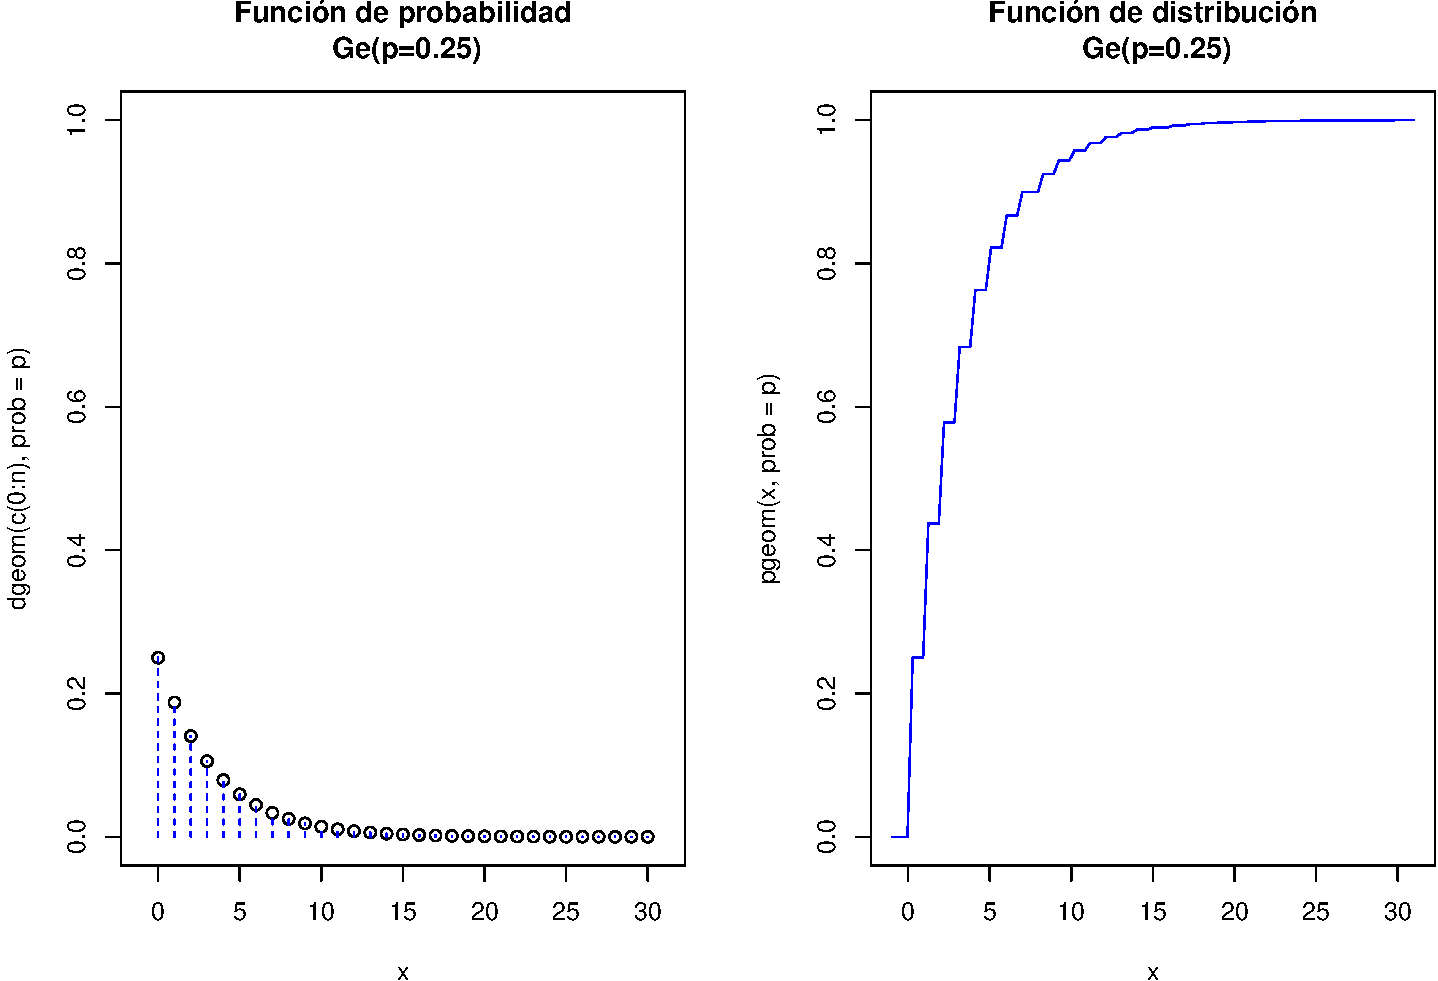
\includegraphics[width=0.8\textwidth,height=\textheight]{Tema_3_1_Notables_files/figure-beamer/graficos22-1.pdf}

}

\end{figure}
\end{frame}

\begin{frame}[fragile]{Cálculos con python}
\protect\hypertarget{cuxe1lculos-con-python}{}
Veamos los cálculos básicos con python para la distribución geométrica
\(Ge(p=0.25)\). scipy.stats implementa la distribución geométrica que
cuenta el número intentos así que empieza en 1

Cargamos la función de la librería

\begin{Shaded}
\begin{Highlighting}[]
\ImportTok{from}\NormalTok{ scipy.stats }\ImportTok{import}\NormalTok{ geom}
\end{Highlighting}
\end{Shaded}

\begin{figure}

{\centering 
\includegraphics[width=0.7\textwidth,height=\textheight]{Tema_3_1_Notables_files/figure-beamer/geom1-1.pdf}

}

\end{figure}
\end{frame}

\begin{frame}[fragile]{Cálculos con python}
\protect\hypertarget{cuxe1lculos-con-python-1}{}
La función de probabilidad es \texttt{geom.pmf(x,p,loc=0)=geom.pmf(x,p)}
es un geométrica que cuenta el número de intentos para obtener el primer
éxito el valor por defecto del último parámetro es \texttt{loc=0}.

Si queremos la que cuenta el número de fracasos para obtener el primer
éxito (la geométrica que empieza en 0) tenemos que usar
\texttt{geom.pmf(x,p,loc=-1)}.

Es decir \texttt{geom.pmf(x,p,loc=-1)=geom.pmf(x-1,p,loc=0)}

Veamos pues los cálculos para la \(Ge(p)\) que empieza en \(0\).

\(P(X=0)=(1-0.25)^0\cdot 0.25^1=0.25\)

\begin{Shaded}
\begin{Highlighting}[]
\NormalTok{geom.pmf(}\DecValTok{0}\NormalTok{,p}\OperatorTok{=}\FloatTok{0.25}\NormalTok{,loc}\OperatorTok{={-}}\DecValTok{1}\NormalTok{)}
\end{Highlighting}
\end{Shaded}

\begin{figure}

{\centering 
\includegraphics[width=0.7\textwidth,height=\textheight]{Tema_3_1_Notables_files/figure-beamer/py_geom_funciones1-3.pdf}

}

\end{figure}

\(P(X\leq 0)=1- (1-0.25)^{0+1}=1-0.75=0.25\)

\begin{Shaded}
\begin{Highlighting}[]
\NormalTok{geom.cdf(}\DecValTok{0}\NormalTok{,p}\OperatorTok{=}\FloatTok{0.25}\NormalTok{,loc}\OperatorTok{={-}}\DecValTok{1}\NormalTok{)}
\end{Highlighting}
\end{Shaded}

\begin{figure}

{\centering 
\includegraphics[width=0.7\textwidth,height=\textheight]{Tema_3_1_Notables_files/figure-beamer/py_geom_funciones2-5.pdf}

}

\end{figure}

\(P(X\leq 4)=1-(1-0.25)^{4+1}=1-0.75=1-0.75^5=0.7626953.\)

\begin{Shaded}
\begin{Highlighting}[]
\NormalTok{geom.cdf(}\DecValTok{4}\NormalTok{,p}\OperatorTok{=}\FloatTok{0.25}\NormalTok{,loc}\OperatorTok{={-}}\DecValTok{1}\NormalTok{)}
\end{Highlighting}
\end{Shaded}

\begin{figure}

{\centering 
\includegraphics[width=0.7\textwidth,height=\textheight]{Tema_3_1_Notables_files/figure-beamer/py_geom_funciones3-7.pdf}

}

\end{figure}

Una muestra aleatoria de tamaño 25 de una \(Ge(0.25)\)

\begin{Shaded}
\begin{Highlighting}[]
\NormalTok{geom.rvs(p}\OperatorTok{=}\FloatTok{0.25}\NormalTok{, size}\OperatorTok{=}\DecValTok{20}\NormalTok{, loc}\OperatorTok{={-}}\DecValTok{1}\NormalTok{)}
\end{Highlighting}
\end{Shaded}

\begin{figure}

{\centering 
\includegraphics[width=0.7\textwidth,height=\textheight]{Tema_3_1_Notables_files/figure-beamer/py_random_binom-9.pdf}

}

\end{figure}
\end{frame}

\begin{frame}[fragile]{Cálculos con python}
\protect\hypertarget{cuxe1lculos-con-python-2}{}
\textbf{Ejercicio}

Qué probabilidades son las que calcula el siguiente código y qué tipo de
variables geométricas son?

\begin{Shaded}
\begin{Highlighting}[]
\NormalTok{geom.cdf(}\BuiltInTok{range}\NormalTok{(}\DecValTok{5}\NormalTok{),p}\OperatorTok{=}\FloatTok{0.3}\NormalTok{,loc}\OperatorTok{=}\DecValTok{0}\NormalTok{)}
\NormalTok{geom.cdf(}\BuiltInTok{range}\NormalTok{(}\DecValTok{5}\NormalTok{),p}\OperatorTok{=}\FloatTok{0.3}\NormalTok{,loc}\OperatorTok{={-}}\DecValTok{1}\NormalTok{)}
\end{Highlighting}
\end{Shaded}

\begin{figure}

{\centering 
\includegraphics[width=0.7\textwidth,height=\textheight]{Tema_3_1_Notables_files/figure-beamer/unnamed-chunk-20-11.pdf}

}

\end{figure}
\end{frame}

\begin{frame}[fragile]{Cálculos con python esperanza y varianza}
\protect\hypertarget{cuxe1lculos-con-python-esperanza-y-varianza}{}
Con python también podemos calcular directamente algunos parámetros
asociado a una función de distribución predefinida

\begin{Shaded}
\begin{Highlighting}[]
\NormalTok{geom.stats(p}\OperatorTok{=}\FloatTok{0.25}\NormalTok{, loc}\OperatorTok{=}\DecValTok{0}\NormalTok{, moments}\OperatorTok{=}\StringTok{\textquotesingle{}mv\textquotesingle{}}\NormalTok{)}
\NormalTok{geom.stats(p}\OperatorTok{=}\FloatTok{0.25}\NormalTok{, loc}\OperatorTok{={-}}\DecValTok{1}\NormalTok{, moments}\OperatorTok{=}\StringTok{\textquotesingle{}mv\textquotesingle{}}\NormalTok{)}
\end{Highlighting}
\end{Shaded}

\begin{figure}

{\centering 
\includegraphics[width=0.7\textwidth,height=\textheight]{Tema_3_1_Notables_files/figure-beamer/py_mean_var_stats-13.pdf}

}

\end{figure}
\end{frame}

\begin{frame}{Cálculos con python esperanza y varianza}
\protect\hypertarget{cuxe1lculos-con-python-esperanza-y-varianza-1}{}
\textbf{Ejercicio}

Comprobad que las medias y las varianzas calculadas en el código
anterior, corresponden a una \(Ge(p=0.3)\) empezando en \(1\) y a una
\(Ge(p=0.3)\) empezando en \(0\).

¿Son las varianzas siempre iguales?
\end{frame}

\begin{frame}[fragile]{Gráficos con python}
\protect\hypertarget{gruxe1ficos-con-python}{}
\begin{Shaded}
\begin{Highlighting}[]
\NormalTok{p }\OperatorTok{=} \FloatTok{0.25}
\NormalTok{x }\OperatorTok{=}\NormalTok{ np.arange(geom.ppf(}\FloatTok{0.01}\NormalTok{, p),geom.ppf(}\FloatTok{0.99}\NormalTok{, p))}
\NormalTok{fig }\OperatorTok{=}\NormalTok{plt.figure(figsize}\OperatorTok{=}\NormalTok{(}\DecValTok{5}\NormalTok{, }\FloatTok{2.7}\NormalTok{))}
\NormalTok{ax }\OperatorTok{=}\NormalTok{ fig.add\_subplot(}\DecValTok{1}\NormalTok{,}\DecValTok{2}\NormalTok{,}\DecValTok{1}\NormalTok{)}
\NormalTok{ax.plot(x, geom.pmf(x, p), }\StringTok{\textquotesingle{}bo\textquotesingle{}}\NormalTok{, ms}\OperatorTok{=}\DecValTok{5}\NormalTok{, label}\OperatorTok{=}\StringTok{\textquotesingle{}geom pmf\textquotesingle{}}\NormalTok{)}
\NormalTok{ax.vlines(x, }\DecValTok{0}\NormalTok{, geom.pmf(x, p), colors}\OperatorTok{=}\StringTok{\textquotesingle{}b\textquotesingle{}}\NormalTok{, lw}\OperatorTok{=}\DecValTok{2}\NormalTok{, alpha}\OperatorTok{=}\FloatTok{0.5}\NormalTok{)}
\ControlFlowTok{for}\NormalTok{ tick }\KeywordTok{in}\NormalTok{ ax.xaxis.get\_major\_ticks():}
\NormalTok{  tick.label.set\_fontsize(}\DecValTok{5}\NormalTok{)}
\ControlFlowTok{for}\NormalTok{ tick }\KeywordTok{in}\NormalTok{ ax.yaxis.get\_major\_ticks():}
\NormalTok{  tick.label.set\_fontsize(}\DecValTok{5}\NormalTok{) }
\NormalTok{ax }\OperatorTok{=}\NormalTok{ fig.add\_subplot(}\DecValTok{1}\NormalTok{,}\DecValTok{2}\NormalTok{,}\DecValTok{2}\NormalTok{)}
\NormalTok{ax.plot(x, geom.cdf(x, p), }\StringTok{\textquotesingle{}bo\textquotesingle{}}\NormalTok{, ms}\OperatorTok{=}\DecValTok{5}\NormalTok{, label}\OperatorTok{=}\StringTok{\textquotesingle{}geom pmf\textquotesingle{}}\NormalTok{)}
\NormalTok{ax.vlines(x, }\DecValTok{0}\NormalTok{, geom.cdf(x, p), colors}\OperatorTok{=}\StringTok{\textquotesingle{}b\textquotesingle{}}\NormalTok{, lw}\OperatorTok{=}\DecValTok{2}\NormalTok{, alpha}\OperatorTok{=}\FloatTok{0.5}\NormalTok{)}
\ControlFlowTok{for}\NormalTok{ tick }\KeywordTok{in}\NormalTok{ ax.xaxis.get\_major\_ticks():}
\NormalTok{  tick.label.set\_fontsize(}\DecValTok{5}\NormalTok{)}
\ControlFlowTok{for}\NormalTok{ tick }\KeywordTok{in}\NormalTok{ ax.yaxis.get\_major\_ticks():}
\NormalTok{  tick.label.set\_fontsize(}\DecValTok{5}\NormalTok{)}
\NormalTok{fig.suptitle(}\StringTok{\textquotesingle{}Distribucion Geometrica\textquotesingle{}}\NormalTok{)}
\NormalTok{plt.show()}
\end{Highlighting}
\end{Shaded}
\end{frame}

\begin{frame}{Gráficos con python}
\protect\hypertarget{gruxe1ficos-con-python-1}{}
\begin{figure}

{\centering 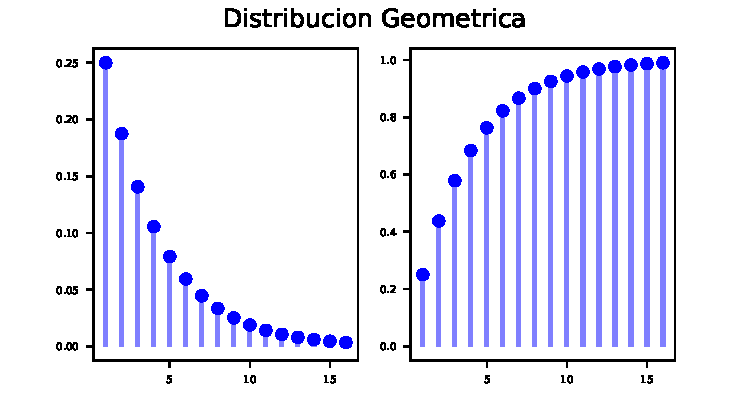
\includegraphics[width=0.7\textwidth,height=\textheight]{Tema_3_1_Notables_files/figure-beamer/unnamed-chunk-21-15.pdf}

}

\end{figure}
\end{frame}

\hypertarget{distribuciuxf3n-binomial-negativa}{%
\section{Distribución binomial
negativa}\label{distribuciuxf3n-binomial-negativa}}

\begin{frame}{El problema de la puerta con dos cerraduras}
\protect\hypertarget{el-problema-de-la-puerta-con-dos-cerraduras}{}
Supongamos que disponemos de 10 llaves distintas y tenemos que abrir una
puerta con \textbf{dos cerraduras}.

Comenzamos por la primera cerradura, de tal forma que cada vez olvidamos
qué llave hemos probado.

Una vez abierta la primera cerradura probamos de igual forma con la
segunda hasta que también la abrimos.

Sea \(X=\) la v.a. que cuenta el número de fracasos hasta abrir la
puerta.

Acertar una llave de la puerta es un experimento Bernoulli con
probabilidad de éxito \(p=0.1\). Lo repetiremos hasta obtener 2 éxitos.
\end{frame}

\begin{frame}{Distribución binomial negativa}
\protect\hypertarget{distribuciuxf3n-binomial-negativa-1}{}
En general tendremos un experimento de Bernoulli con probabilidad de
éxito \(0<p<1\) tal que:

\begin{itemize}
\tightlist
\item
  Repetimos el experimento hasta obtener el \(n\)-ésimo éxito ¡¡abrir la
  maldita puerta!!.
\item
  Sea \(X\) la v.a. que cuenta el número fallos hasta abrir la puerta,
  es decir, hasta conseguir el n-ésimo éxito. Notemos que no contamos
  los éxitos, solo contamos los fracasos
\end{itemize}
\end{frame}

\begin{frame}{Distribución binomial negativa}
\protect\hypertarget{distribuciuxf3n-binomial-negativa-2}{}
Si representamos como es habitual un suceso como una cadena de F's y
E's, para \(n=2\), algunos sucesos elementales serán:
\[\small{\{EE,FEE,EFE, FFEE,FEFE,EFFE,FFFEE,FFEFE,FEFFE,EFFFE\}.}\]

Calculemos algunas probabilidades para \(n=2\): \[
\small{
\begin{array}{rl}
P(X=0) & =P(\{EE\})=p^2, \\
P(X=1) & =P(\{FEE,EFE\})=2\cdot (1-p)\cdot p^2, \\
P(X=2) & =P(\{FFEE,FEFE,EFFE\})=3\cdot (1-p)^2\cdot p^2, \\
P(X=3) & =P(\{FFFEE,FFEFE,FEFFE,EFFFE\})=4\cdot (1-p)^3\cdot p^2.
\end{array}
}
\]
\end{frame}

\begin{frame}{Distribución binomial negativa}
\protect\hypertarget{distribuciuxf3n-binomial-negativa-3}{}
En general su función de probabilidad es

\[
P_{X}(k)=P(X=k)=\left\{\begin{array}{ll}
     {k+n-1\choose n-1} \cdot (1-p)^{k}\cdot p^n & \mbox{si } k=0,1,\ldots\\
     0 & \mbox{en otro caso}\end{array}\right.
\]
\end{frame}

\begin{frame}{Distribución binomial negativa}
\protect\hypertarget{distribuciuxf3n-binomial-negativa-4}{}
Una v.a. con este tipo de distribución recibe el nombre de
\textbf{binomial negativa} y la denotaremos por \(BN(n,p)\).

Notemos que \(BN(1,p)=Ge(p)\).
\end{frame}

\begin{frame}{Distribución binomial negativa}
\protect\hypertarget{distribuciuxf3n-binomial-negativa-5}{}
\textbf{Demostración}

Justifiquemos el resultado. Sea \(X\) una \(BN(n,p)\) y sea
\(k=0,1,2,\ldots\).

\[\scriptsize{P(X=k)=P(\mbox{Todas las cadenas de E's y F' con $k$ F, con $n$ E y acabadas en E})}\]

\[
\scriptsize{\overbrace{\underbrace{\overbrace{EFFF\ldots EEF}^{n-1 \quad \mbox{Éxitos}.}}}_{k \quad\mbox{Fracasos}}^{k+n-1\mbox{ posiciones}}E}
\]

De estas cadenas hay tantas como maneras de elegir de entre las
\(k+n-1\) primeras posiciones \(n-1\) para colocar los éxitos. Esta
cantidad es el número binomial \({k+n-1\choose n-1}.\)
\end{frame}

\begin{frame}{Números binomiales negativos}
\protect\hypertarget{nuxfameros-binomiales-negativos}{}
Números binomiales negativos

Dados dos enteros positivos \(n\) y \(k\) se define el número binomial
negativo como

\[\binom{-n}{k}=\frac{(-n)(-n-1)\cdots (-n-k+1)}{k!}.\]

Los números binomiales negativos generalizan la fórmula de Newton para
exponentes negativos: \[
(t+1)^{-n}=\sum_{k=0}^{+\infty}\left(\begin{array}{c} -n
\\ k\end{array}\right) t^{k}
\]
\end{frame}

\begin{frame}[fragile]{Números binomiales negativos}
\protect\hypertarget{nuxfameros-binomiales-negativos-1}{}
\texttt{R} usa la función \texttt{choose} para calcular números
binomiales, sean negativos o no. Veámoslo con un ejemplo:

\[
\begin{array}{rl}
{-6\choose 4}&=\frac{-6\cdot (-6-1)\cdot \cdot (-6-2)\cdot (-6-3) }{4!}\\
&=  \frac{-6\cdot(-7)\cdot (-8)\cdot (-9)}{24}\\
&= \frac{3024}{24}=126.
\end{array}
\]

Si realizamos el cálculo con \texttt{R} obtenemos el mismo resultado:

\begin{Shaded}
\begin{Highlighting}[]
\FunctionTok{choose}\NormalTok{(}\SpecialCharTok{{-}}\DecValTok{6}\NormalTok{,}\DecValTok{4}\NormalTok{)}
\end{Highlighting}
\end{Shaded}

\begin{verbatim}
[1] 126
\end{verbatim}
\end{frame}

\begin{frame}{Esperanza de una \(BN(n,p)\)}
\protect\hypertarget{esperanza-de-una-bnnp}{}
Su \textbf{esperanza es}

\[E(X)=\sum_{k=0}^{+\infty} k\cdot {k+n-1\choose n-1} \cdot (1-p)^{k}\cdot p^n=n\cdot\frac{1-p}{p}.\]

La \textbf{esperanza de \(X^2\) es}

\[E(X^2)=\sum_{k=0}^{+\infty} k^2\cdot {k+n-1\choose n-1} \cdot (1-p)^{k}\cdot p^n=n\cdot\frac{1-p}{p^2}+\left(n\cdot \frac{1-p}{p}\right)^2.\]
\end{frame}

\begin{frame}{Varianza de una \(BN(n,p)\)}
\protect\hypertarget{varianza-de-una-bnnp}{}
Por último la \textbf{varianza es}

\[
Var(X)=E(X^2)-E(X)^2=
\]

\[=n\cdot \frac{1-p}{p^2}+\left(n\cdot \frac{1-p}{p}\right)^2-\left(n\cdot \frac{1-p}{p}\right)^2=
n\cdot \frac{1-p}{p^2}.\]

y por tanto la desviación típica es

\[\sqrt{Var(X)} = \frac{\sqrt{n(1-p)}}{p}\]
\end{frame}

\begin{frame}{Resumen distribución Binomial Negativa \(BN(n,p)\)}
\protect\hypertarget{resumen-distribuciuxf3n-binomial-negativa-bnnp}{}
\renewcommand{\arraystretch}{1.8}
\begin{table}
\centering
\begin{tabular}{|l|}
\hline\rowcolor{LightBlue}
 $X=$ Número de fracasos antes de conseguir el $n$-ésimo éxito, $P(\mbox{Éxito})=p$. $BN(n,p)$ 
\\\hline
$D_X=\{0,1,2,3\ldots\}$  \\\hline
$P_X(k)=P(X=k)=\left\{\begin{array}{ll} {k+n-1\choose n-1} \cdot (1-p)^{k}\cdot p^n, & \mbox{si }  k=0,1,\ldots \\ 0, & \mbox{en otro caso.}\end{array}\right.$\\\hline
$
F_X(x)=P(X\leq x)=
\left\{
\begin{array}{ll} 0, & \mbox{si } x<0\\\displaystyle\sum_{i=0}^{k} P(X=i) & \mbox{si  }\left\{\begin{array}{l}k\leq x< k+1,\\k=0,1,2,\ldots\end{array}\right.\end{array}\right.$ 
\\\hline
$E(X)=n\cdot\frac{1-p}{p}$;  $Var(X)=n\cdot \frac{1-p}{p^2}.$ \\\hline
\end{tabular}
\end{table}
\end{frame}

\begin{frame}{Ejemplo puerta dos cerraduras \(BN(n=2,p=0.1)\).}
\protect\hypertarget{ejemplo-puerta-dos-cerraduras-bnn2p0.1.}{}
\textbf{Ejercicio: Puerta con dos cerraduras}

Recordemos nuestra puerta con dos cerraduras que se abren
secuencialmente. Tenemos un manojo de 10 llaves casi idénticas de manera
que cada vez que probamos una llave olvidamos qué llave hemos usado.

Sea \(X\) la v.a que nos da el número de intentos fallidos hasta abrir
abrir la puerta.
\end{frame}

\begin{frame}{Ejemplo \(BN(n,p)\)}
\protect\hypertarget{ejemplo-bnnp}{}
Estamos interesado en modelar este problema. La preguntas son:

\begin{enumerate}
\tightlist
\item
  ¿Cuál es la distribución de probabilidad de \(X\) la v.a que nos da el
  número fallos hasta abrir la puerta?
\item
  ¿Cuál es la función de probabilidad y de distribución de \(X\)?
\item
  ¿Cuál es la probabilidad de fallar exactamente 5 veces antes de abrir
  la puerta?
\item
  ¿Cuál es la probabilidad de fallar más de 4?
\item
  ¿Cuál es el número esperado de fallos? ¿Y su desviación típica?
\end{enumerate}
\end{frame}

\begin{frame}{Ejemplo dos cerraduras \(BN(n=2,p=0.1)\).}
\protect\hypertarget{ejemplo-dos-cerraduras-bnn2p0.1.}{}
\textbf{Solución 1.} ¿Cuál es la distribución de probabilidad de \(X\)
la v.a que nos da el número fallos hasta abrir la puerta?

Bajo estados condiciones tenemos que la probabilidad de ``éxito'' de
cada intento es \(p=\frac{1}{10}=0.1\). Como cada vez \emph{olvidamos}
qué llave hemos probado, cada intento será independiente del anterior.

Así que la variable \(X\) que queremos modelar cuenta el número fallos
de repeticiones sucesivas e independientes de un experimento
\(Ber(p=0.1)\) hasta conseguir 2 éxitos en un experimento.

Por lo tanto podemos asegurar que \(X\) sigue un distribución
\(BN(n=2,p=0.1).\)
\end{frame}

\begin{frame}{Ejemplo \(BN(n=2,p=0.1)\)}
\protect\hypertarget{ejemplo-bnn2p0.1}{}
\textbf{Solución 2.} ¿Cuál es la función de probabilidad y de
distribución del \(X\)?

En general la función de probabilidad de una \(BN(n,p)\) es

\[
P_X(k)=P(X=k)=
\left\{
\begin{array}{cc} 
{k+n-1\choose n-1} \cdot (1-p)^{k}\cdot p^n & \mbox{si }  k=0,1,\ldots \\ 0 & \mbox{en otro caso.}\end{array}\right.
\]

Si aplicamos la expresión anterior para \(n=2\) y \(p=0.1\), obtenemos:
\[
P_X(k)=P(X=k)=
\left\{
\begin{array}{cc} 
{k+2-1\choose 2-1} \cdot 0.9^{k}\cdot 0.1^2 & \mbox{si }  k=0,1,2,\ldots \\ 0 & \mbox{en otro caso.}\end{array}\right.
\]
\end{frame}

\begin{frame}{Ejemplo \(BN(n=2,p=0.1)\)}
\protect\hypertarget{ejemplo-bnn2p0.1-1}{}
Simplificando

\[
P_X(X=k)=P(X=k)=
\left\{
\begin{array}{cc} 
0.01\cdot (k+1)\cdot 0.9^{k}, & \mbox{si }  k=0,1,2,\ldots \\ 0 & \mbox{en otro caso.}\end{array}\right.
\]

La función de distribución en general es

\[
F_X(x)=P(X\leq x)=
\left\{
\begin{array}{ll}
0 & \mbox{si } x<0 \\
\displaystyle\sum_{i=0}^{k }{i+n-1\choose n-1} \cdot (1-p)^{i+n-1}\cdot p^n 
& \mbox{si }\left\{\begin{array}{l} k\leq x< k+1\\k=0,1,2,\ldots\end{array}\right. 
\end{array}
\right.
\]
\end{frame}

\begin{frame}{Ejemplo \(BN(n=2,p=0.1)\)}
\protect\hypertarget{ejemplo-bnn2p0.1-2}{}
Simplificando para \(n=2\), \(p=0.1\).

\[
F_X(x)=P(X\leq x)=
\left\{
\begin{array}{ll}
0, & \mbox{si } x<0, \\
\displaystyle\sum_{i=0}^{k }0.01\cdot (i+1) \cdot 0.9^{i+1},
& \mbox{si }\left\{\begin{array}{l} k\leq x< k+1,\\k=0,1,2,\ldots\end{array}\right. 
\end{array}
\right.
\]

\textbf{Solución 3.} ¿Cuál es la probabilidad de fallar exactamente 5
veces antes de abrir la puerta?

\[
P(X=5)= 0.01\cdot (5+1) \cdot 0.9^{5}= 0.06 \cdot 0.9^{5}= 0.0354294.
\]
\end{frame}

\begin{frame}{Ejemplo \(BN(n=2,p=0.1)\)}
\protect\hypertarget{ejemplo-bnn2p0.1-3}{}
\textbf{Solución 4.} ¿Cuál es la probabilidad de fallar más de 4?

Nos piden que\\
\[
P(X>4)=1-P(X\leq 4).
\]

Calculemos primero \(P(X\leq 4):\)

\[
\begin{array}{rl}
P(X\leq 4) &=  \displaystyle\sum_{x=0}^{4} P(X=x)=P(X=0)+P(X=1)+P(X=2)+P(X=3)+P(X=4)\\
&= 0.01\cdot (0+1) \cdot 0.9^{0}+0.01\cdot (1+1) \cdot 0.9^{1}+0.01\cdot (2+1) \cdot 0.9^{2} \\ &\ \ 
+0.01\cdot (3+1) \cdot 0.9^{3} + 0.01\cdot (4+1) \cdot 0.9^{4} \\ & =
0.01 +0.018+0.0243+0.02916+0.032805 = 0.114265.
\end{array}
\]
\end{frame}

\begin{frame}{Ejemplo \(BN(n=2,p=0.1)\)}
\protect\hypertarget{ejemplo-bnn2p0.1-4}{}
Por lo tanto

\[
P(X>4)=1-P(X\leq 4)=1-0.114265=
0.885735.
\]

\textbf{Solución 5.} ¿Cuál es el número esperado de fallos? ¿Y su
desviación típica?

Como \(X\) sigue una ley \(BN(n=2,p=0.1)\)

\[E(X)=n\cdot \frac{1-p}{p}=2\cdot \frac{1-0.1}{0.1}=18.\]

El número de fallos esperado es 18. La varianza es

\[
Var(X)=n\cdot\frac{1-p}{p^2}=2 \cdot \frac{1-0.1}{0.1^2}=180,
\]

y su desviación típica \(\sqrt{180}=13.41641.\)
\end{frame}

\begin{frame}[fragile]{Cálculos con R}
\protect\hypertarget{cuxe1lculos-con-r-2}{}
La función de \texttt{R} que calcula la función de probabilidad de la
binomial negativa con sus parámetros básicos es:

\begin{verbatim}
dnbinom(x, size, prob,...)`
\end{verbatim}

donde \texttt{size} (\(n\)) es el número de éxitos y \texttt{prob}
(\(p\)), la probabilidad de éxito.

Así en el ejemplo de la puerta con dos cerraduras, \(X\) es una
\(BN(n=size=2,p=prob=0.1)\). Por ejemplo, \(P(X=5)\) que hemos calculado
en el ejemplo anterior, vale:

\begin{Shaded}
\begin{Highlighting}[]
\FunctionTok{dnbinom}\NormalTok{(}\DecValTok{5}\NormalTok{,}\AttributeTok{size=}\DecValTok{2}\NormalTok{,}\AttributeTok{p=}\FloatTok{0.1}\NormalTok{)}
\end{Highlighting}
\end{Shaded}

\begin{verbatim}
[1] 0.0354294
\end{verbatim}
\end{frame}

\begin{frame}[fragile]{Cálculos con R}
\protect\hypertarget{cuxe1lculos-con-r-3}{}
De forma similar calculamos calculamos \(P(X\leq 4)\),
\(P(X>4)=1-P(X\leq 4)\) y \(P(X>4)\).

\begin{Shaded}
\begin{Highlighting}[]
\FunctionTok{pnbinom}\NormalTok{(}\DecValTok{4}\NormalTok{,}\AttributeTok{size=}\DecValTok{2}\NormalTok{,}\AttributeTok{p=}\FloatTok{0.1}\NormalTok{)}
\end{Highlighting}
\end{Shaded}

\begin{verbatim}
[1] 0.114265
\end{verbatim}

\begin{Shaded}
\begin{Highlighting}[]
\DecValTok{1}\SpecialCharTok{{-}}\FunctionTok{pnbinom}\NormalTok{(}\DecValTok{4}\NormalTok{,}\AttributeTok{size=}\DecValTok{2}\NormalTok{,}\AttributeTok{p=}\FloatTok{0.1}\NormalTok{)}
\end{Highlighting}
\end{Shaded}

\begin{verbatim}
[1] 0.885735
\end{verbatim}

\begin{Shaded}
\begin{Highlighting}[]
\FunctionTok{pnbinom}\NormalTok{(}\DecValTok{4}\NormalTok{,}\AttributeTok{size=}\DecValTok{2}\NormalTok{,}\AttributeTok{p=}\FloatTok{0.1}\NormalTok{,}\AttributeTok{lower.tail=}\ConstantTok{FALSE}\NormalTok{)}
\end{Highlighting}
\end{Shaded}

\begin{verbatim}
[1] 0.885735
\end{verbatim}
\end{frame}

\begin{frame}[fragile]{Cálculos con python}
\protect\hypertarget{cuxe1lculos-con-python-3}{}
La función con python es \texttt{nbinom.pmf(k,\ n,\ p,\ loc)}. Hay que
cargarla desde \texttt{scpi.stats}

\begin{Shaded}
\begin{Highlighting}[]
\ImportTok{from}\NormalTok{ scipy.stats }\ImportTok{import}\NormalTok{ nbinom}
\end{Highlighting}
\end{Shaded}

Recordemos que de nuevo se cumple que

\begin{Shaded}
\begin{Highlighting}[]
\NormalTok{nbinom.pmf(k, n, p, loc) }\OperatorTok{=}\NormalTok{ nbinom.pmf(k}\OperatorTok{{-}}\NormalTok{loc, n, p)\textasciigrave{}}
\end{Highlighting}
\end{Shaded}
\end{frame}

\begin{frame}[fragile]{Cálculos \(BN(n,p)\) con python}
\protect\hypertarget{cuxe1lculos-bnnp-con-python}{}
\begin{Shaded}
\begin{Highlighting}[]
\NormalTok{nbinom.pmf(k}\OperatorTok{=}\DecValTok{5}\NormalTok{,n}\OperatorTok{=}\DecValTok{2}\NormalTok{,p}\OperatorTok{=}\FloatTok{0.1}\NormalTok{)}
\end{Highlighting}
\end{Shaded}

\begin{verbatim}
0.0354294
\end{verbatim}

\begin{Shaded}
\begin{Highlighting}[]
\NormalTok{nbinom.pmf(k}\OperatorTok{=}\DecValTok{5}\NormalTok{,n}\OperatorTok{=}\DecValTok{2}\NormalTok{,p}\OperatorTok{=}\FloatTok{0.1}\NormalTok{,loc}\OperatorTok{=}\DecValTok{0}\NormalTok{)}
\end{Highlighting}
\end{Shaded}

\begin{verbatim}
0.0354294
\end{verbatim}

\begin{Shaded}
\begin{Highlighting}[]
\NormalTok{nbinom.cdf(k}\OperatorTok{=}\DecValTok{4}\NormalTok{,n}\OperatorTok{=}\DecValTok{2}\NormalTok{,p}\OperatorTok{=}\FloatTok{0.1}\NormalTok{)}
\end{Highlighting}
\end{Shaded}

\begin{verbatim}
0.11426500000000002
\end{verbatim}

\begin{Shaded}
\begin{Highlighting}[]
\DecValTok{1}\OperatorTok{{-}}\NormalTok{nbinom.cdf(k}\OperatorTok{=}\DecValTok{4}\NormalTok{,n}\OperatorTok{=}\DecValTok{2}\NormalTok{,p}\OperatorTok{=}\FloatTok{0.1}\NormalTok{)}
\end{Highlighting}
\end{Shaded}

\begin{verbatim}
0.8857349999999999
\end{verbatim}
\end{frame}

\begin{frame}[fragile]{Cálculos \(BN(n,p)\) con python}
\protect\hypertarget{cuxe1lculos-bnnp-con-python-1}{}
Generemos 100 observaciones aleatorias de una \(BN(n=2,0.1)\). Es decir
serán las veces que hemos fallado hasta abrir la puerta 100 veces.

\begin{Shaded}
\begin{Highlighting}[]
\NormalTok{nbinom.rvs(n}\OperatorTok{=}\DecValTok{2}\NormalTok{, p}\OperatorTok{=}\FloatTok{0.1}\NormalTok{, size}\OperatorTok{=}\DecValTok{100}\NormalTok{)}
\end{Highlighting}
\end{Shaded}

\begin{verbatim}
array([35,  0, 12, 13,  2, 29, 17, 27, 14,  6, 18, 73,  8,  1, 14,  4, 11,
        3,  4, 27,  7, 21, 26, 11,  9, 17, 29,  3, 24, 10,  5,  3, 22, 10,
       39, 11, 23, 54, 12, 31, 14, 20,  0, 33, 24, 15, 21, 17, 20,  2, 13,
       17, 11, 24,  3, 23,  0, 17, 34, 23,  4, 28, 46, 42, 26, 10, 14,  3,
       23, 18,  1, 30, 21, 67, 45, 12, 26, 12,  1,  7, 23,  9,  1, 19, 12,
       10, 20, 21, 21, 33, 13, 26,  9, 26,  7,  8, 26,  3,  0, 70],
      dtype=int64)
\end{verbatim}
\end{frame}

\begin{frame}[fragile]{Cálculos \(BN(n,p)\) con python}
\protect\hypertarget{cuxe1lculos-bnnp-con-python-2}{}
La \textbf{esperanza} y la \textbf{varianza}de una \(BN(n=2,0.1)\)
valen:

\begin{Shaded}
\begin{Highlighting}[]
\NormalTok{n, p}\OperatorTok{=}\DecValTok{2}\NormalTok{,}\FloatTok{0.1}
\NormalTok{params }\OperatorTok{=}\NormalTok{ nbinom.stats(n,p,moments}\OperatorTok{=}\StringTok{\textquotesingle{}mv\textquotesingle{}}\NormalTok{)}
\BuiltInTok{print}\NormalTok{(}\StringTok{"E(X)=}\SpecialCharTok{\{m\}}\StringTok{"}\NormalTok{.}\BuiltInTok{format}\NormalTok{(m}\OperatorTok{=}\NormalTok{params[}\DecValTok{0}\NormalTok{]))}
\end{Highlighting}
\end{Shaded}

\begin{verbatim}
E(X)=18.0
\end{verbatim}

\begin{Shaded}
\begin{Highlighting}[]
\BuiltInTok{print}\NormalTok{(}\StringTok{"Var(X)=}\SpecialCharTok{\{v\}}\StringTok{"}\NormalTok{.}\BuiltInTok{format}\NormalTok{(v}\OperatorTok{=}\NormalTok{params[}\DecValTok{1}\NormalTok{]))}
\end{Highlighting}
\end{Shaded}

\begin{verbatim}
Var(X)=179.99999999999997
\end{verbatim}
\end{frame}

\begin{frame}[fragile]{Gráficas de la binomial negativa con R}
\protect\hypertarget{gruxe1ficas-de-la-binomial-negativa-con-r}{}
El siguiente código de R dibuja las función de probabilidad y la de
distribución de una \(BN(n=2,p=0.1)\)

\begin{Shaded}
\begin{Highlighting}[]
\FunctionTok{par}\NormalTok{(}\AttributeTok{mfrow=}\FunctionTok{c}\NormalTok{(}\DecValTok{1}\NormalTok{,}\DecValTok{2}\NormalTok{))}
\NormalTok{aux}\OtherTok{=}\FunctionTok{rep}\NormalTok{(}\DecValTok{0}\NormalTok{,}\DecValTok{22}\NormalTok{)}
\NormalTok{aux[}\FunctionTok{seq}\NormalTok{(}\DecValTok{2}\NormalTok{,}\DecValTok{22}\NormalTok{,}\DecValTok{2}\NormalTok{)]}\OtherTok{=}\FunctionTok{dnbinom}\NormalTok{(}\FunctionTok{c}\NormalTok{(}\DecValTok{0}\SpecialCharTok{:}\DecValTok{10}\NormalTok{),}\AttributeTok{size=}\DecValTok{2}\NormalTok{,}\AttributeTok{prob=}\FloatTok{0.1}\NormalTok{)}
\FunctionTok{plot}\NormalTok{(}\AttributeTok{x=}\FunctionTok{c}\NormalTok{(}\DecValTok{0}\SpecialCharTok{:}\DecValTok{10}\NormalTok{),}\AttributeTok{y=}\FunctionTok{dnbinom}\NormalTok{(}\FunctionTok{c}\NormalTok{(}\DecValTok{0}\SpecialCharTok{:}\DecValTok{10}\NormalTok{),}\AttributeTok{size=}\DecValTok{2}\NormalTok{,}\AttributeTok{prob=}\FloatTok{0.1}\NormalTok{),}
  \AttributeTok{ylim=}\FunctionTok{c}\NormalTok{(}\DecValTok{0}\NormalTok{,}\DecValTok{1}\NormalTok{),}\AttributeTok{xlim=}\FunctionTok{c}\NormalTok{(}\SpecialCharTok{{-}}\DecValTok{1}\NormalTok{,}\DecValTok{11}\NormalTok{),}\AttributeTok{xlab=}\StringTok{"x"}\NormalTok{,}
  \AttributeTok{main=}\StringTok{"Función de probabilidad}\SpecialCharTok{\textbackslash{}n}\StringTok{ BN(n=2,p=0.1)"}\NormalTok{)}
\FunctionTok{lines}\NormalTok{(}\AttributeTok{x=}\FunctionTok{rep}\NormalTok{(}\DecValTok{0}\SpecialCharTok{:}\DecValTok{10}\NormalTok{,}\AttributeTok{each=}\DecValTok{2}\NormalTok{),}\AttributeTok{y=}\NormalTok{aux, }\AttributeTok{type =} \StringTok{"h"}\NormalTok{, }\AttributeTok{lty =} \DecValTok{2}\NormalTok{,}\AttributeTok{col=}\StringTok{"blue"}\NormalTok{)}
\FunctionTok{curve}\NormalTok{(}\FunctionTok{pnbinom}\NormalTok{(x,}\AttributeTok{size=}\DecValTok{2}\NormalTok{,}\AttributeTok{prob=}\DecValTok{0}\NormalTok{,}\DecValTok{1}\NormalTok{),}
  \AttributeTok{xlim=}\FunctionTok{c}\NormalTok{(}\SpecialCharTok{{-}}\DecValTok{1}\NormalTok{,}\DecValTok{11}\NormalTok{),}\AttributeTok{col=}\StringTok{"blue"}\NormalTok{,}
  \AttributeTok{main=}\StringTok{"Función de distribución}\SpecialCharTok{\textbackslash{}n}\StringTok{ BN(n=2,p=0.1)"}\NormalTok{)}
\FunctionTok{par}\NormalTok{(}\AttributeTok{mfrow=}\FunctionTok{c}\NormalTok{(}\DecValTok{1}\NormalTok{,}\DecValTok{1}\NormalTok{))}
\end{Highlighting}
\end{Shaded}
\end{frame}

\begin{frame}{Gráficas de la binomial negativa con R}
\protect\hypertarget{gruxe1ficas-de-la-binomial-negativa-con-r-1}{}
\begin{figure}

{\centering 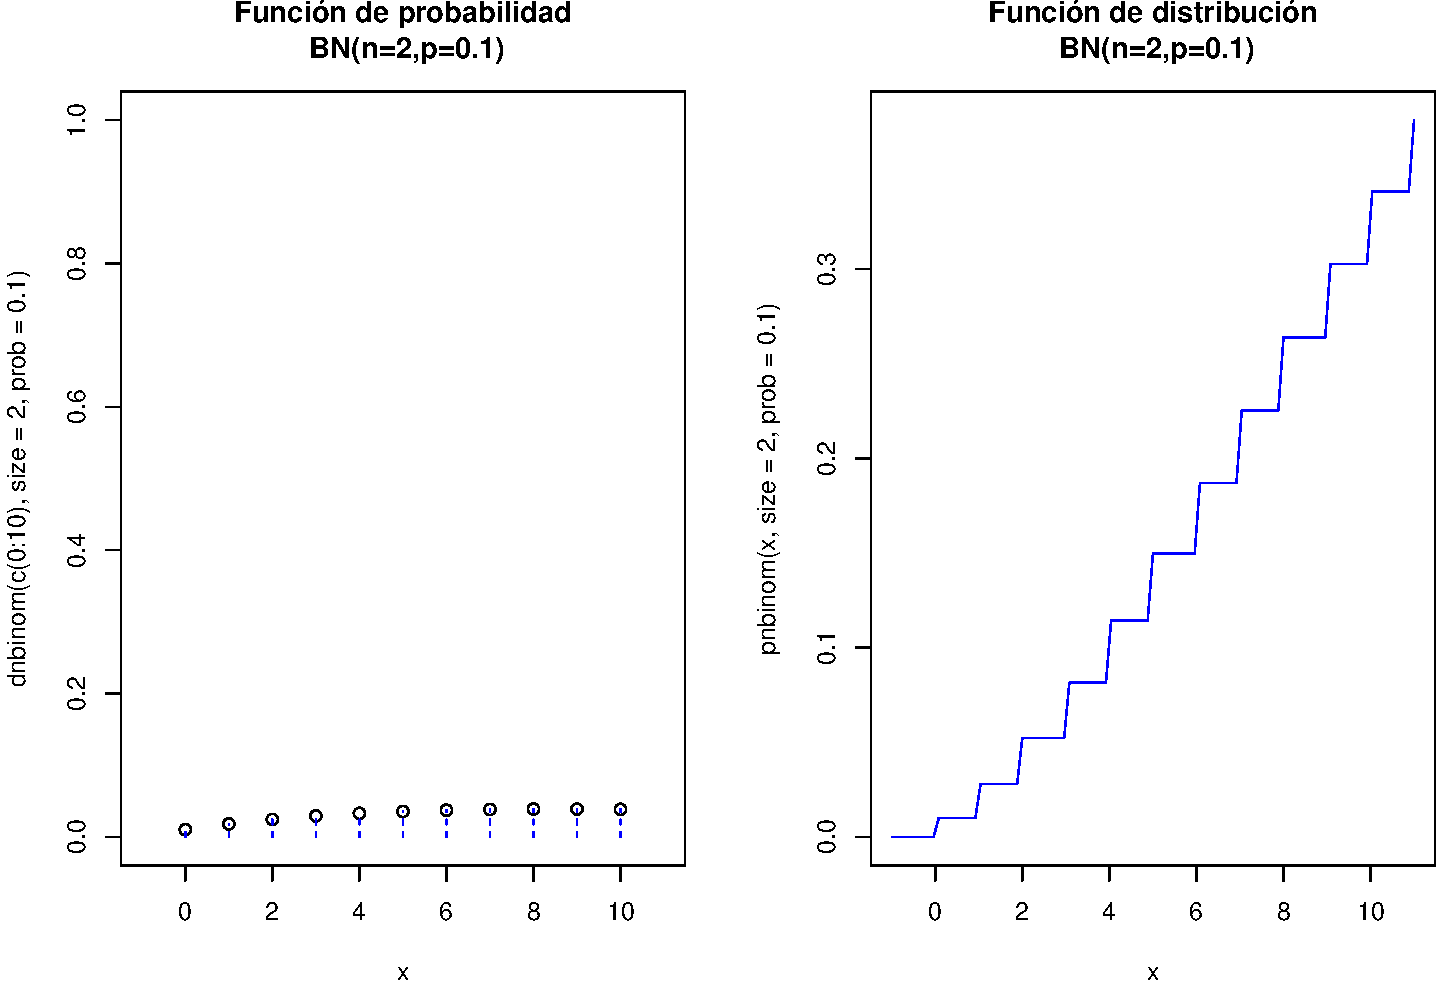
\includegraphics[width=0.7\textwidth,height=\textheight]{Tema_3_1_Notables_files/figure-beamer/unnamed-chunk-32-1.pdf}

}

\end{figure}
\end{frame}

\begin{frame}[fragile]{Gráficos de la binomial negativa con python}
\protect\hypertarget{gruxe1ficos-de-la-binomial-negativa-con-python}{}
\textbf{Ejercicio}

Buscad en los manuales de python cómo se dibuja la función de
probabilidad y de distribución de una binomial. negativa

Necesitamos de nuevo más librerías

\begin{Shaded}
\begin{Highlighting}[]
\ImportTok{import}\NormalTok{ numpy }\ImportTok{as}\NormalTok{ np}
\ImportTok{from}\NormalTok{ scipy.stats }\ImportTok{import}\NormalTok{ nbinom}
\ImportTok{import}\NormalTok{ matplotlib.pyplot }\ImportTok{as}\NormalTok{ plt}
\end{Highlighting}
\end{Shaded}
\end{frame}

\begin{frame}[fragile]{Gráficos de la binomial negativa con python}
\protect\hypertarget{gruxe1ficos-de-la-binomial-negativa-con-python-1}{}
\begin{Shaded}
\begin{Highlighting}[]
\NormalTok{n, p }\OperatorTok{=} \DecValTok{10}\NormalTok{, }\FloatTok{0.25}
\NormalTok{x }\OperatorTok{=}\NormalTok{ np.arange(}\DecValTok{0}\NormalTok{,nbinom.ppf(}\FloatTok{0.99}\NormalTok{, n, p))}
\NormalTok{fig }\OperatorTok{=}\NormalTok{plt.figure(figsize}\OperatorTok{=}\NormalTok{(}\DecValTok{5}\NormalTok{, }\FloatTok{2.7}\NormalTok{))}
\NormalTok{ax }\OperatorTok{=}\NormalTok{ fig.add\_subplot(}\DecValTok{1}\NormalTok{,}\DecValTok{2}\NormalTok{,}\DecValTok{1}\NormalTok{)}
\NormalTok{ax.plot(x, nbinom.pmf(x, n, p), }\StringTok{\textquotesingle{}bo\textquotesingle{}}\NormalTok{, ms}\OperatorTok{=}\DecValTok{5}\NormalTok{, label}\OperatorTok{=}\StringTok{\textquotesingle{}nbinom pmf\textquotesingle{}}\NormalTok{)}
\NormalTok{ax.vlines(x, }\DecValTok{0}\NormalTok{, nbinom.pmf(x, n, p), colors}\OperatorTok{=}\StringTok{\textquotesingle{}b\textquotesingle{}}\NormalTok{, lw}\OperatorTok{=}\DecValTok{2}\NormalTok{, alpha}\OperatorTok{=}\FloatTok{0.5}\NormalTok{)}
\ControlFlowTok{for}\NormalTok{ tick }\KeywordTok{in}\NormalTok{ ax.xaxis.get\_major\_ticks():}
\NormalTok{  tick.label.set\_fontsize(}\DecValTok{5}\NormalTok{)}
\ControlFlowTok{for}\NormalTok{ tick }\KeywordTok{in}\NormalTok{ ax.yaxis.get\_major\_ticks():}
\NormalTok{  tick.label.set\_fontsize(}\DecValTok{5}\NormalTok{) }
\NormalTok{ax }\OperatorTok{=}\NormalTok{ fig.add\_subplot(}\DecValTok{1}\NormalTok{,}\DecValTok{2}\NormalTok{,}\DecValTok{2}\NormalTok{)}
\NormalTok{ax.plot(x, nbinom.cdf(x, n, p), }\StringTok{\textquotesingle{}bo\textquotesingle{}}\NormalTok{, ms}\OperatorTok{=}\DecValTok{5}\NormalTok{, label}\OperatorTok{=}\StringTok{\textquotesingle{}nbinom pmf\textquotesingle{}}\NormalTok{)}
\NormalTok{ax.vlines(x, }\DecValTok{0}\NormalTok{, nbinom.cdf(x, n, p), colors}\OperatorTok{=}\StringTok{\textquotesingle{}b\textquotesingle{}}\NormalTok{, lw}\OperatorTok{=}\DecValTok{2}\NormalTok{, alpha}\OperatorTok{=}\FloatTok{0.5}\NormalTok{)}
\ControlFlowTok{for}\NormalTok{ tick }\KeywordTok{in}\NormalTok{ ax.xaxis.get\_major\_ticks():}
\NormalTok{  tick.label.set\_fontsize(}\DecValTok{5}\NormalTok{)}
\ControlFlowTok{for}\NormalTok{ tick }\KeywordTok{in}\NormalTok{ ax.yaxis.get\_major\_ticks():}
\NormalTok{  tick.label.set\_fontsize(}\DecValTok{5}\NormalTok{)}
\NormalTok{fig.suptitle(}\StringTok{\textquotesingle{}Distribucion Binomial Negativa\textquotesingle{}}\NormalTok{)}
\NormalTok{plt.show()}
\end{Highlighting}
\end{Shaded}
\end{frame}

\begin{frame}{Gráficos de la binomial negativa con python}
\protect\hypertarget{gruxe1ficos-de-la-binomial-negativa-con-python-2}{}
\begin{figure}

{\centering 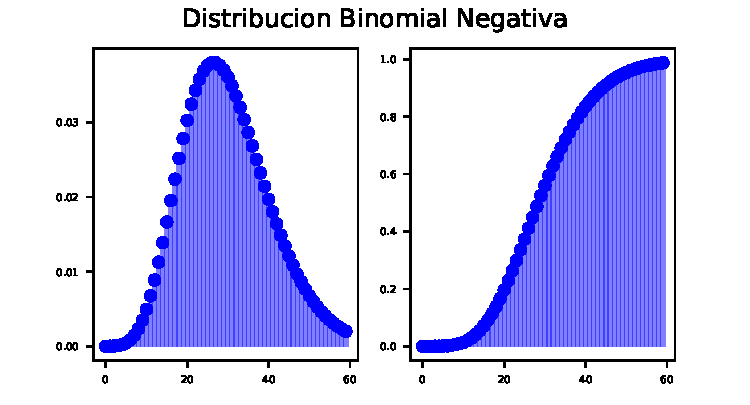
\includegraphics[width=0.7\textwidth,height=\textheight]{Tema_3_1_Notables_files/figure-beamer/negativa_py_show-1.pdf}

}

\end{figure}
\end{frame}

\begin{frame}{Ejercicio: Acceso aleatorio a un sistema con triple
clave.}
\protect\hypertarget{ejercicio-acceso-aleatorio-a-un-sistema-con-triple-clave.}{}
\textbf{Sistema con tres claves de acceso}

Supongamos que tenemos un sistema informático tiene un programa de
seguridad que genera accesos con claves de 3 dígitos
\(000,001,\ldots 999\). En total 1000 posibilidades.

Como una clave de tres dígitos es fácil de romper proponemos considerar
tres claves consecutivas de acceso al sistema, cada una de 3 dígitos.

Para acceder al sistema hay que dar las tres claves de forma consecutiva
y por orden.

Es decir hasta que no averiguamos la primera clave no pasamos a la
segunda clave.

Supongamos que cada vez que ponemos las dos claves olvidamos el
resultado y seguimos poniendo claves al azar hasta adivinar la
contraseña.

Así hasta conseguir entrar en el sistema.

Sea \(X\) la v.a que nos da el número de fallos antes de entrar en el
sistema.
\end{frame}

\begin{frame}{Ejercicio acceso aleatorio a un sistema con triple clave.}
\protect\hypertarget{ejercicio-acceso-aleatorio-a-un-sistema-con-triple-clave.-1}{}
Estamos interesados en modelar este problema. La preguntas son:

\begin{enumerate}
\tightlist
\item
  ¿Cuál es la distribución de probabilidad de \(X\), la v.a que nos da
  el número de fallos antes de acceder al sistema.
\item
  ¿Cuál es la función de probabilidad y de distribución del \(X\)?
\item
  ¿Cuál es la probabilidad de fallar 150 veces antes de acceder en el
  sistema?
\item
  ¿Cuál es la probabilidad de fallar más de 150 veces antes de entrar en
  el sistema?
\item
  ¿Cuál es el número esperado de fallos antes de acceder al sistema? ¿Y
  su varianza?
\end{enumerate}
\end{frame}

\begin{frame}{Ejemplo \(BN(r,p)\)}
\protect\hypertarget{ejemplo-bnrp}{}
\textbf{Solución 1.} ¿Cuál es la distribución de probabilidad de \(X\),
la v.a que nos da el número de fallos antes de acceder al sistema?

Bajo estados condiciones tenemos que la probabilidad de ``éxito'' de
cada intento es \(p=\frac{1}{1000}=0.001\). Y como cada vez
\emph{olvidamos} en los dígitos cada intento será independiente del
anterior.

Así que la variable \(X\) cuenta el número de fracasos independientes
hasta conseguir 3 éxitos en un experimento \(Ber(p=0.001)\) por lo tanto
\(X\) sigue un distribución \(BN(n=3,p=0.001).\)
\end{frame}

\begin{frame}{Ejemplo \(BN(r,p)\)}
\protect\hypertarget{ejemplo-bnrp-1}{}
\textbf{Solución 2.} ¿Cuál es la función de probabilidad y de
distribución del \(X\)

En general la función de probabilidad de una \(BN(n,p)\) es

\[
P_X(X=x)=P(X=x)=
\left\{
\begin{array}{cc} 
{x+n-1\choose n-1} \cdot (1-p)^{x}\cdot p^n & \mbox{si }  x=0,1,\ldots \\ 0 & \mbox{en otro caso.}\end{array}\right.
\] En particular la función de probabilidad de una \(BN(n=3,p=0.001)\)
es

\[
P_X(X=x)=P(X=x)=
\left\{
\begin{array}{cc} 
{x+2\choose 2} \cdot 0.999^{x}\cdot 0.001^3 & \mbox{si }  x=0,1,2,\ldots \\ 0 & \mbox{en otro caso.}\end{array}\right.
\]
\end{frame}

\begin{frame}[fragile]{Solución ejemplo \(BN(n=3,p=0.001)\)}
\protect\hypertarget{soluciuxf3n-ejemplo-bnn3p0.001}{}
\textbf{Solución 3.} ¿Cuál es la probabilidad de fallar 150 veces antes
de acceder en el sistema?

Nos piden

\[
\scriptsize{P(X=150)= {152\choose 2} \cdot 0.999^{150}\cdot 0.001^3.}
\]

Lo calcularemos operando con R

\begin{Shaded}
\begin{Highlighting}[]
\FunctionTok{choose}\NormalTok{(}\DecValTok{152}\NormalTok{,}\DecValTok{2}\NormalTok{)}\SpecialCharTok{*}\FloatTok{0.999}\SpecialCharTok{\^{}}\DecValTok{150}\SpecialCharTok{*}\FloatTok{0.001}\SpecialCharTok{\^{}}\DecValTok{3}
\end{Highlighting}
\end{Shaded}

\begin{verbatim}
[1] 9.876743e-06
\end{verbatim}

\begin{Shaded}
\begin{Highlighting}[]
\FunctionTok{dnbinom}\NormalTok{(}\DecValTok{150}\NormalTok{,}\AttributeTok{size=}\DecValTok{3}\NormalTok{,}\AttributeTok{p=}\FloatTok{0.001}\NormalTok{)}
\end{Highlighting}
\end{Shaded}

\begin{verbatim}
[1] 9.876743e-06
\end{verbatim}
\end{frame}

\begin{frame}[fragile]{Solución ejemplo \(BN(n=3,p=0.001)\)}
\protect\hypertarget{soluciuxf3n-ejemplo-bnn3p0.001-1}{}
\textbf{Solución 3.} ¿Cuál es la probabilidad de fallar 150 veces antes
de acceder en el sistema?

Nos piden, lo resolveremos con python

\[
P(X=150)= {152\choose 2} \cdot 0.999^{150}\cdot 0.001^3
\]

\begin{Shaded}
\begin{Highlighting}[]
\ImportTok{from}\NormalTok{  scipy.special }\ImportTok{import}\NormalTok{ binom}
\NormalTok{binom(}\DecValTok{152}\NormalTok{,}\DecValTok{2}\NormalTok{)}\OperatorTok{*}\FloatTok{0.999}\OperatorTok{**}\DecValTok{150}\OperatorTok{*}\FloatTok{0.001}\OperatorTok{**}\DecValTok{3}
\end{Highlighting}
\end{Shaded}

\begin{verbatim}
9.876743459670526e-06
\end{verbatim}

\begin{Shaded}
\begin{Highlighting}[]
\NormalTok{nbinom.pmf(}\DecValTok{150}\NormalTok{,n}\OperatorTok{=}\DecValTok{3}\NormalTok{,p}\OperatorTok{=}\FloatTok{0.001}\NormalTok{)}
\end{Highlighting}
\end{Shaded}

\begin{verbatim}
9.876743459670532e-06
\end{verbatim}
\end{frame}

\begin{frame}{Solución ejemplo \(BN(n,p)\)}
\protect\hypertarget{soluciuxf3n-ejemplo-bnnp}{}
\textbf{Solución 4.} ¿Cuál es la probabilidad de fallar más de 150 veces
antes de entrar en el sistema?

\[P(X>150)=1-P(X\leq 150)\]

Calculemos \(P(X\leq 150)\)

\begin{eqnarray*}
P(X\leq 150) &=& P(X=0)+P(X=1)+P(X=2)+\ldots+P(X=150)\\
&=& \sum_{k=0}^{150} {k+3-1\choose 3-1} \cdot (0.999)^{k}\cdot 0.001^3\ldots = \ldots =\ensuremath{5.2320035\times 10^{-4}}
\end{eqnarray*}
\end{frame}

\begin{frame}[fragile]{Solución ejemplo \(BN(n,p)\)}
\protect\hypertarget{soluciuxf3n-ejemplo-bnnp-1}{}
Con R

\begin{Shaded}
\begin{Highlighting}[]
\FunctionTok{pnbinom}\NormalTok{(}\DecValTok{150}\NormalTok{,}\DecValTok{3}\NormalTok{,}\FloatTok{0.001}\NormalTok{)}
\end{Highlighting}
\end{Shaded}

\begin{verbatim}
[1] 0.0005232003
\end{verbatim}

Con python

\begin{Shaded}
\begin{Highlighting}[]
\NormalTok{nbinom.cdf(}\DecValTok{150}\NormalTok{,n}\OperatorTok{=}\DecValTok{3}\NormalTok{,p}\OperatorTok{=}\FloatTok{0.001}\NormalTok{)}
\end{Highlighting}
\end{Shaded}

\begin{verbatim}
0.0005232003490824064
\end{verbatim}

\begin{frame}{Solución ejemplo \(BN(n,p)\)}
\protect\hypertarget{soluciuxf3n-ejemplo-bnnp-2}{}
El valor pedido será pues: \[
P(X>150)=1-P(X\leq 150)=1-\ensuremath{5.2320035\times 10^{-4}}=0.9994768.
\] Vemos que es muy probable que fallemos más de 150 veces antes de
entrar en el sistema.
\end{frame}
\end{frame}

\begin{frame}[fragile]{Solución ejemplo \(BN(n,p)\)}
\protect\hypertarget{soluciuxf3n-ejemplo-bnnp-3}{}
\textbf{Solución 5.} ¿Cuál es el número esperado de fallos antes de
acceder al sistema? ¿Y su desviación típica?

\[E(X)=n\cdot \frac{1-p}{p}=3\cdot \frac{1- 0.001}{0.001}=2997.\]
\[Var(X)=n\cdot \frac{1-p}{p^2}=3\cdot \frac{1- 0.001^2}{0.001^2}=\ensuremath{2.997\times 10^{6}}.\]

Con python

\begin{Shaded}
\begin{Highlighting}[]
\NormalTok{params }\OperatorTok{=}\NormalTok{ nbinom.stats(n}\OperatorTok{=}\DecValTok{3}\NormalTok{,p}\OperatorTok{=}\FloatTok{0.001}\NormalTok{,moments}\OperatorTok{=}\StringTok{\textquotesingle{}mv\textquotesingle{}}\NormalTok{)}
\BuiltInTok{print}\NormalTok{(}\StringTok{"E(X) = }\SpecialCharTok{\{m\}}\StringTok{"}\NormalTok{.}\BuiltInTok{format}\NormalTok{(m}\OperatorTok{=}\NormalTok{params[}\DecValTok{0}\NormalTok{]))}
\end{Highlighting}
\end{Shaded}

\begin{verbatim}
E(X) = 2997.0
\end{verbatim}

\begin{Shaded}
\begin{Highlighting}[]
\BuiltInTok{print}\NormalTok{(}\StringTok{"Var(X) = }\SpecialCharTok{\{v\}}\StringTok{"}\NormalTok{.}\BuiltInTok{format}\NormalTok{(v}\OperatorTok{=}\NormalTok{params[}\DecValTok{1}\NormalTok{]))}
\end{Highlighting}
\end{Shaded}

\begin{verbatim}
Var(X) = 2997000.0
\end{verbatim}
\end{frame}

\begin{frame}{¿Tres claves de tres dígitos o una de 9 dígitos?}
\protect\hypertarget{tres-claves-de-tres-duxedgitos-o-una-de-9-duxedgitos}{}
\textbf{Ejercicio}

Supongamos que ponemos una sola clave de 9 dígitos. Estudiemos en este
caso la variable aleatoria que da el número de fallos antes de entrar en
el sistema y comparemos los resultados.

Si seguimos suponiendo que cada vez ponemos la contraseña al azar pero
esta vez con una clave de 9 dígitos. La probabilidad de éxito será ahora
\(p=\frac{1}{10^{9}}\).

Si llamamos \(X_9\) a la variable aleatoria que nos da el número de
fallos antes de entra en el sistema seguirá una distribución
\(Ge(p=\frac{1}{10^9}=0.000000001)\).
\end{frame}

\begin{frame}{Qué da más seguridad ¿tres claves de tres dígitos o una de
9 dígitos?}
\protect\hypertarget{quuxe9-da-muxe1s-seguridad-tres-claves-de-tres-duxedgitos-o-una-de-9-duxedgitos}{}
Su valor esperado es

\[
E(X_9)=\frac{1-p}{p}=\frac{1-0.000000001}{0.000000001}=\ensuremath{10\times 10^{8}}.
\]

\(1000 000 000\) son 1000 millones de fallos esperados hasta abrir la
puerta.

Recordemos que con tres contraseñas de 3 dígitos el valor esperado de
fallos es

\[3\cdot \frac{1-0.001}{0.001}=2997.\]

Por lo tanto, desde el punto de vista de la seguridad, es mejor una
clave larga de 9 dígitos que tres cortas si escribimos las contraseñas
al azar.
\end{frame}

\hypertarget{distribuciuxf3n-de-poisson}{%
\section{Distribución de Poisson}\label{distribuciuxf3n-de-poisson}}

\begin{frame}{Distribución Poisson}
\protect\hypertarget{distribuciuxf3n-poisson}{}
Diremos que una v.a. discreta \(X\) con \(X(\Omega)=\mathbf{N}\) tiene
distribución de Poisson con parámetro \(\lambda>0\), y lo denotaremos
por \(Po(\lambda)\) si su función de probabilidad es:

\[
P_{X}(x)=P(X=x)=
\left\{\begin{array}{ll}
\frac{\lambda^x}{x!} e^{-\lambda}& \mbox{ si } x=0,1,\ldots\\
0 & \mbox{en otro caso}\end{array}\right..
\]
\end{frame}

\begin{frame}{Distribución Poisson}
\protect\hypertarget{distribuciuxf3n-poisson-1}{}
Usando que el desarrollo en serie de Taylor de la función exponencial es
\[
e^{\lambda}=\sum_{x=0}^{+\infty} \frac{\lambda^x}{x!},
\] es fácil comprobar que la suma de la función de probabilidad en todos
los valores del dominio de \(X\), o sea, los enteros positivos, vale 1.

Además recordemos que dado \(x\in\mathbb{R}-\{0\}\) se tiene que

\[
\lim_{n\to\infty} \left(1+\frac{x}{n}\right)^n=e^x.
\]
\end{frame}

\begin{frame}{Distribución Poisson}
\protect\hypertarget{distribuciuxf3n-poisson-2}{}
Usando la expresión anterior para \(x=-\lambda\), tenemos:

\[
\lim_{n\to\infty} \left(1-\frac{\lambda}{n}\right)^n=\lim_{n\to\infty} \left(1+\frac{-\lambda}{n}\right)^n=e^{-\lambda}.
\]
\end{frame}

\begin{frame}{La distribución de Poisson como ``límite'' de una
binomial.}
\protect\hypertarget{la-distribuciuxf3n-de-poisson-como-luxedmite-de-una-binomial.}{}
La distribución de Poisson
(\href{https://es.wikipedia.org/wiki/Sim\%C3\%A9on_Denis_Poisson}{Siméon
Denis Poisson}) aparece en el conteo de determinados eventos que se
producen en un intervalo de tiempo o en el espacio.

Supongamos que nuestra variable de interés es \(X\), el número de
eventos en el intervalo de tiempo \((0,t]\), como por ejemplo el número
de llamadas a un \emph{call center} en una hora donde suponemos que se
cumplen las siguientes condiciones:
\end{frame}

\begin{frame}{La distribución Poisson como ``límite'' de una binomial.}
\protect\hypertarget{la-distribuciuxf3n-poisson-como-luxedmite-de-una-binomial.}{}
\begin{enumerate}
\tightlist
\item
  El número promedio de eventos en el intervalo \((0,t]\) es
  \(\lambda>0\).
\item
  Es posible dividir el intervalo de tiempo en un gran número de
  subintervalos (denotemos por \(n\) al número de intervalos) de forma
  que:

  \begin{itemize}
  \tightlist
  \item
    La probabilidad de que se produzcan dos o más eventos en un
    subintervalo es despreciable.
  \item
    El número de ocurrencias de eventos en un intervalo es independiente
    del número de ocurrencias en otro intervalo.
  \item
    La probabilidad de que un evento ocurra en un subintervalo es
    \(p_n=\frac{\lambda}{n}\)·
  \end{itemize}
\end{enumerate}
\end{frame}

\begin{frame}{La distribución Poisson como ``límite'' de una binomial.}
\protect\hypertarget{la-distribuciuxf3n-poisson-como-luxedmite-de-una-binomial.-1}{}
Bajo estas condiciones, podemos considerar que el número de eventos en
el intervalo \((0,t]\) será el número de ``éxitos'' en \(n\)
repeticiones independientes de un proceso Bernoulli de parámetro \(p_n\)

Entonces si \(n\to\infty\) y \(p_n\cdot n\) se mantiene igual a
\(\lambda\) resulta que la función de probabilidad de \(X\) se puede
escribir como
\end{frame}

\begin{frame}{La distribución Poisson como ``límite'' de una binomial.}
\protect\hypertarget{la-distribuciuxf3n-poisson-como-luxedmite-de-una-binomial.-2}{}
\[
\begin{array}{rl}
P(X_n=k)&=\left(\begin{array}{c} n\\ k\end{array}\right) \cdot p_n^k\cdot  (1-p_n)^{n-k}
\\
&= {n\choose k}\cdot \left(\frac{\lambda}{n}\right)^{k}\cdot \left(1-\frac{\lambda}{n}\right)^{n-k}\\
&=
\frac{\lambda^k}{k!}\cdot\frac{n!}{(n-k)!\cdot n^k}\cdot
\left(1-\frac{\lambda}{n}\right)^{n}\cdot \left(1-\frac{\lambda}{n}\right)^{-k}.
\end{array}
\]
\end{frame}

\begin{frame}{La distribución Poisson como ``límite'' de una binomial.}
\protect\hypertarget{la-distribuciuxf3n-poisson-como-luxedmite-de-una-binomial.-3}{}
Si hacemos tender \(n\) hacia \(\infty\), obtenemos: \[
\lim_{n\to \infty} P(X_n=k) = \lim_{n\to \infty} \frac{\lambda^k}{k!}\cdot\frac{n!}{(n-k)!\cdot n^k} \cdot
\left(1-\frac{\lambda}{n}\right)^{n}\cdot \left(1-\frac{\lambda}{n}\right)^{-k}.
\]

Calculemos el límite de algunos de los factores de la expresión

\[
\displaystyle\lim_{n\to \infty}\frac{n!}{(n-k)!\cdot n^k}= \lim_{n\to \infty}\frac{n\cdot (n-1)\cdots (n-k-1)}{n^k}
=\lim_{n\to \infty}\frac{n^{k}+\cdots}{n^k}=1.
\]
\end{frame}

\begin{frame}{La distribución Poisson como ``límite'' de una binomial.}
\protect\hypertarget{la-distribuciuxf3n-poisson-como-luxedmite-de-una-binomial.-4}{}
\[
\lim_{n\to \infty} \left(1-\frac{\lambda}{n}\right)^{n}=e^{-\lambda}
\]

Y también teniendo en cuanta que \(k\) es constante.

\[
\lim_{n\to \infty} \left(1-\frac{\lambda}{n}\right)^{-k}=\lim_{n\to \infty} 1^{-k}=\lim_{n\to \infty}  1=1.
\]
\end{frame}

\begin{frame}{La distribución Poisson como ``límite'' de una binomial.}
\protect\hypertarget{la-distribuciuxf3n-poisson-como-luxedmite-de-una-binomial.-5}{}
Para acabar

\[
\displaystyle\lim_{n\to\infty} P(X_n=k)=
\lim_{n\to\infty} \left(\begin{array}{c} n\\ k\end{array}\right)
\cdot p_n^k \cdot (1-p_n)^{n-k}= \frac{\lambda^k}{k!}\cdot 1 \cdot e^{-\lambda}\cdot 1=\frac{\lambda^k}{k!}\cdot e^{-\lambda}.
\]

Lo que confirma que límite de una serie de variables
\(B(n,p_n=\frac{\lambda}{n})\) sigue una ley \(Po(\lambda)\).
\end{frame}

\begin{frame}{Procesos de Poisson}
\protect\hypertarget{procesos-de-poisson}{}
Lo interesante de las variables Poisson es que podemos modificar (si el
modelo lo permite) el intervalo de tiempo \((0,t]\) en el que contamos
los eventos.

Claro que esto no tiene que poder ser así.

Pero en general si la variable es poisson en \((0,t]\) también lo será
en cualquier subintervalo \((0,t']\) para todo \(t'\) tal que
\(0<t'<t\).

Así que podremos definir una serie de variables \(X_t\) de distribución
\(Po(\lambda\cdot t)\).
\end{frame}

\begin{frame}{Procesos de Poisson}
\protect\hypertarget{procesos-de-poisson-1}{}
Definición procesos de Poisson

Consideremos un experimento \emph{Poisson} con \(\lambda\) igual al
promedio de eventos en una unidad de tiempo (u.t.).

Si \(t\) es una cantidad de tiempo en u.t., la v.a. \(X_{t}\)=numero de
eventos en el intervalo \((0,t]\) es una \(Po(\lambda\cdot t)\).

El conjunto de variables \(\{X_t\}_{t>0}\) recibe el nombre de
\textbf{proceso de Poisson}.
\end{frame}

\begin{frame}{Resumen distribución Poisson \(X\equiv Po(\lambda)\)}
\protect\hypertarget{resumen-distribuciuxf3n-poisson-xequiv-polambda}{}
\renewcommand{\arraystretch}{1.75}
\begin{table}
\centering
\begin{tabular}{|l|}
\hline\rowcolor{LightBlue}
$X$ con distribución  Poisson  de media o promedio $\lambda$,  $Po(\lambda)$
\\\hline
$D_X=\{0,1,\ldots \}$ \\\hline
$P_X(x)=P(X=x)=\left\{\begin{array}{ll}  \frac{\lambda^x}{x!}e^{-\lambda} & \mbox{ si } x=0,1,\ldots\\ 0  & \mbox{ en otro caso.}\end{array}\right.$\\\hline
$\scriptstyle F_X(x)=P(X\leq X)=\left\{\begin{array}{ll} 0 & \mbox{si } x<0\\\displaystyle\scriptstyle\sum_{i=0}^{k} P(X=i)= \displaystyle\scriptstyle\sum_{i=0}^{k} \frac{\lambda^i}{i!}\cdot e^{-\lambda} & \mbox{si  }\left\{\begin{array}{l}\scriptstyle k\leq x< k+1\\\scriptstyle k=0,1,2,\ldots\end{array}\right.\end{array}\right.$
     \\\hline
$E(X)=\lambda$; $Var(X)=\lambda$\\\hline
\end{tabular}
\end{table}
\end{frame}

\begin{frame}{Resumen proceso Poisson \(X_t\equiv Po(\lambda\cdot t)\)}
\protect\hypertarget{resumen-proceso-poisson-x_tequiv-polambdacdot-t}{}
\renewcommand{\arraystretch}{1.75}
\begin{table}
\centering
\begin{tabular}{|l|}
\hline\rowcolor{LightBlue}
$X_t=$ número de eventos en el intervalo $(0,t]$  $Po(\lambda\cdot t)$  donde  $\lambda$ promedio por u.t. 
\\\hline
$D_X=\{0,1,\ldots \}$ \\\hline
$P_X(x)=P(X=x)=\left\{\begin{array}{ll}  \frac{(\lambda\cdot t)^x}{x!}e^{-\lambda\cdot t} & \mbox{ si } x=0,1,\ldots\\ 0  & \mbox{ en otro caso.}\end{array}\right.$\\\hline
$\scriptstyle F_X(x)=P(X\leq X)=\left\{\begin{array}{ll} 0 & \mbox{si } x<0\\\displaystyle\scriptstyle\sum_{i=0}^{k} P(X=i)= \displaystyle\scriptstyle\sum_{i=0}^{k} \frac{(\lambda\cdot t)^i}{i!}\cdot e^{-\lambda\cdot t} & \mbox{si  }\left\{\begin{array}{l}\scriptstyle k\leq x< k+1\\\scriptstyle k=0,1,2,\ldots\end{array}\right.\end{array}\right.$

   \\\hline
$E(X)=\lambda\cdot t$; $Var(X)=\lambda\cdot t$\\\hline
\end{tabular}
\end{table}
\end{frame}

\begin{frame}{Aproximación de la distribución binomial por la Poisson}
\protect\hypertarget{aproximaciuxf3n-de-la-distribuciuxf3n-binomial-por-la-poisson}{}
Bajo el punto de vista anterior y si \(p\) es pequeño y \(n\)
suficientemente grande la distribución \(B(n,p)\) se aproxima a una
\(Po(\lambda=n\cdot p)\).

Existen distintos criterios (ninguno perfecto) de cuando la aproximación
es buena.

Por ejemplo si

\[n\geq 20\mbox{ o mejor }n\geq 30, n\cdot p < 10 \mbox{ y } p\leq 0.05,\]

la aproximación de una \(B(n,p)\) por una \(Po(n\cdot p)\) es buena.
Sobre todo para los valores cercanos a \(E(X)=\lambda\).

Condición deseable \(n\geq 20\), \(n\cdot p < 10\), \(p\leq 0.05\).
\end{frame}

\begin{frame}{Ejemplo \(Po(\lambda)\)}
\protect\hypertarget{ejemplo-polambda}{}
\textbf{Ejemplo}: Trampa insectos.

La conocida
\href{https://es.wikipedia.org/wiki/Insecticida_el\%C3\%A9ctrico}{lámpara
antiinsectos o insecticida eléctrico} atrae a los insectos voladores con
una luz ultravioleta y los mata por electrocución.

Consideremos la v.a. \(X\) que cuenta el número de insectos caídos en la
trampa en una hora. Supongamos que el número promedio de insectos que
captura la trampa en una hora es \(E(X)=20\) y que podemos admitir que
\(X\) sigue una ley de probabilidad \(Po(\lambda=20)\).

Nos piden

\begin{enumerate}
\tightlist
\item
  Comentar de forma breve si se cumplen intuitivamente las condiciones
  para tener una distribución Poisson.
\item
  Escribir de forma explicita la función de probabilidad y de
  distribución de \(X\).
\item
  Calculad la probabilidad de que en una hora caigan en la trampa
  exactamente 21 insectos.
\item
  Calculad la probabilidad de que en una hora caigan en la trampa al
  menos 6 insectos.
\item
  ¿Cuál es el valor esperando, la varianza y la desviación típica de
  \(X\)?
\end{enumerate}
\end{frame}

\begin{frame}{Ejemplo \(Po(\lambda)\)}
\protect\hypertarget{ejemplo-polambda-1}{}
\textbf{Solución 1.} Comentar de forma breve si se cumplen
intuitivamente las condiciones para tener una distribución Poisson.

\begin{enumerate}
\tightlist
\item
  El número promedio de eventos en el intervalo \((0,1]\), una hora es
  \(\lambda=20>0\).
\item
  Es posible dividir el intervalo de tiempo de una hora en un gran
  número de subintervalos (denotemos por \(n\) al número de intervalos)
  de forma que:

  \begin{itemize}
  \tightlist
  \item
    La probabilidad de que se produzcan dos o más electrocuciones un
    subintervalo es despreciable. No es posible que dos mosquitos se
    electrocuten al mismo tiempo.
  \item
    El número de ocurrencias, electrocuciones de insectos, en un
    intervalo es independiente del número de electrocuciones en otro
    intervalo.
  \item
    La probabilidad de que un evento ocurra en un subintervalo es
    \(p_n=\frac{\lambda}{n}\)· Podemos dividir los 20 insectos promedio
    entre los \(n\) intervalos (trozo de hora) de forma que
    \(p_n=\frac{\lambda}{n}\).
  \item
    Por ejemplo si \(n=60\) tenemos que
    \(p_n=\frac{20}{60}=\frac{1}{3}\). La probabilidad de que en un
    minuto la trampa chisporrotee es \(\frac{1}{3}\).
  \end{itemize}
\end{enumerate}
\end{frame}

\begin{frame}{Ejemplo \(Po(\lambda)\)}
\protect\hypertarget{ejemplo-polambda-2}{}
\textbf{Solución 2.} Escribid de forma explicita la función de
probabilidad y de distribución de \(X\).

La distribución de probabilidad de un \(Po(\lambda)\) es

\[
P_X(x)=P(X=x)=\left\{\begin{array}{ll}  \frac{\lambda^x}{x!}e^{-\lambda} & \mbox{ si } x=0,1,\ldots\\ 0  & \mbox{ en otro caso.}\end{array}\right.
\]

En nuestro caso, \(\lambda =20\):

\[
P_X(x)=P(X=x)=\left\{\begin{array}{ll}\frac{20^x}{x!}e^{-20} & \mbox{ si } x=0,1,\ldots\\ 0  & \mbox{ en otro caso.}\end{array}\right.
\]
\end{frame}

\begin{frame}{Ejemplo \(Po(\lambda)\)}
\protect\hypertarget{ejemplo-polambda-3}{}
La función de distribución es

\[
F_X(x)=P(X\leq X)=
\left\{\begin{array}{ll} 
0 & \mbox{si } x<0\\
\displaystyle\sum_{i=0}^{k} P(X=i)=\sum_{i=0}^{k}\frac{\lambda^i}{i!}\cdot e^{-\lambda} & \mbox{si  }
\left\{\begin{array}{l}
k\leq x< k+1\\k=0,1,2,\ldots
\end{array}
\right.
\end{array}
\right.
\]

En nuestro caso \[
F_X(x)=P(X\leq X)=
\left\{\begin{array}{ll} 
0 & \mbox{si } x<0\\
\displaystyle\sum_{i=0}^{k} P(X=i)=\sum_{i=0}^{k}\frac{20^i}{i!}\cdot e^{-20} & \mbox{si  }
\left\{\begin{array}{l}
k\leq x< k+1\\k=0,1,2,\ldots
\end{array}
\right.
\end{array}
\right.
\]
\end{frame}

\begin{frame}[fragile]{Ejemplo \(Po(\lambda)\)}
\protect\hypertarget{ejemplo-polambda-4}{}
\textbf{Solución 3.} Calculad la probabilidad de que en una hora caigan
en la trampa exactamente 21 insectos.

Nos piden la probabilidad siguiente: \[
P(X=21)=\frac{20^{21}}{21!} e^{-20}=0.0846051.
\]

Para realizar el cálculo anterior, podemos usar \texttt{R} como
calculadora o usar la función \texttt{dpois} que nos calcula la función
de distribución de la variable de Poisson:

\begin{Shaded}
\begin{Highlighting}[]
\DecValTok{20}\SpecialCharTok{\^{}}\DecValTok{21}\SpecialCharTok{/}\FunctionTok{factorial}\NormalTok{(}\DecValTok{21}\NormalTok{)}\SpecialCharTok{*}\FunctionTok{exp}\NormalTok{(}\SpecialCharTok{{-}}\DecValTok{20}\NormalTok{)}
\end{Highlighting}
\end{Shaded}

\begin{verbatim}
[1] 0.08460506
\end{verbatim}

\begin{Shaded}
\begin{Highlighting}[]
\FunctionTok{dpois}\NormalTok{(}\DecValTok{21}\NormalTok{,}\AttributeTok{lambda =} \DecValTok{20}\NormalTok{)}
\end{Highlighting}
\end{Shaded}

\begin{verbatim}
[1] 0.08460506
\end{verbatim}
\end{frame}

\begin{frame}{Ejemplo \(Po(\lambda)\)}
\protect\hypertarget{ejemplo-polambda-5}{}
\textbf{Solución 4.} Calculad la probabilidad de que en una hora caigan
en la trampa al menos 6 insectos.

Nos piden la probabilidad siguiente: \[
\begin{array}{rl}
 P(X\geq 6)&=1- P(X<6)=1-P(X\leq 5)=1-F_X(5)=1-\displaystyle\sum_{x=0}^{5} \frac{20^{x}}{x!}\cdot e^{-20}\\
 &=
 1-\left(\frac{20^{0}}{0!}\cdot e^{-20}+\frac{20^{1}}{1!}\cdot e^{-20}+\frac{20^{2}}{2!}\cdot e^{-20}+\frac{20^{3}}{3!}\cdot e^{-20}+\frac{20^{4}}{4!}\cdot e^{-20}+\frac{20^{5}}{5!}\cdot e^{-20}\right)\\
 &=
 1-e^{-20}\cdot \left(1+20+\frac{400}{4}+\frac{8000}{6}+\frac{160000}{24}+\frac{3200000}{120}\right)\\
 &=
 1-e^{-20} \cdot \left(\frac{1 \cdot 120+20\cdot 120+400\cdot 30+8000\cdot 20+160000\cdot 24+3200000\cdot 1}{120}\right)\\
 &= 1-e^{-20}\cdot\left(\frac{4186520}{120}\right)=1-\ensuremath{7.1908841\times 10^{-5}} =0.9999281.
\end{array}
\]
\end{frame}

\begin{frame}{Ejemplo \(Po(\lambda)\)}
\protect\hypertarget{ejemplo-polambda-6}{}
\textbf{Solución 5.} ¿Cuál es el valor esperado, la varianza y la
desviación típica de \(X\)?

El valor esperado del número de insectos caídos en la trampa en una hora
es

\[E(X)=\lambda=20\]

Su varianza es \[Var(X)=\lambda=20\]

y su desviación típica vale
\[\sqrt{Var(X)}=+\sqrt{\lambda}=+\sqrt{20}=4.47214.\]
\end{frame}

\begin{frame}[fragile]{Cálculos con R}
\protect\hypertarget{cuxe1lculos-con-r-4}{}
Consideremos por ejemplo una v.a. \(X\) con distribución
\(Po(\lambda=3)\). Calculemos \(P_X(0)=P(X=0), P_X(1)=P(X=1)\) con
\texttt{R}:

\begin{Shaded}
\begin{Highlighting}[]
\FunctionTok{dpois}\NormalTok{(}\DecValTok{0}\NormalTok{,}\AttributeTok{lambda =} \DecValTok{3}\NormalTok{)}
\end{Highlighting}
\end{Shaded}

\begin{verbatim}
[1] 0.04978707
\end{verbatim}

\begin{Shaded}
\begin{Highlighting}[]
\FunctionTok{dpois}\NormalTok{(}\DecValTok{1}\NormalTok{,}\AttributeTok{lambda =} \DecValTok{3}\NormalTok{)}
\end{Highlighting}
\end{Shaded}

\begin{verbatim}
[1] 0.1493612
\end{verbatim}
\end{frame}

\begin{frame}[fragile]{Cálculos con R}
\protect\hypertarget{cuxe1lculos-con-r-5}{}
Si quisiéramos hallar la función de distribución en los mismos valores
anteriores, \(F_X(0)=P(X\leq 0), F_X(1)=P(X\leq 1)\), haríamos lo
siguiente:

\begin{Shaded}
\begin{Highlighting}[]
\FunctionTok{ppois}\NormalTok{(}\DecValTok{0}\NormalTok{,}\AttributeTok{lambda =} \DecValTok{3}\NormalTok{)}
\end{Highlighting}
\end{Shaded}

\begin{verbatim}
[1] 0.04978707
\end{verbatim}

\begin{Shaded}
\begin{Highlighting}[]
\FunctionTok{ppois}\NormalTok{(}\DecValTok{1}\NormalTok{,}\AttributeTok{lambda =} \DecValTok{3}\NormalTok{)}
\end{Highlighting}
\end{Shaded}

\begin{verbatim}
[1] 0.1991483
\end{verbatim}

\begin{Shaded}
\begin{Highlighting}[]
\FunctionTok{dpois}\NormalTok{(}\DecValTok{0}\NormalTok{,}\AttributeTok{lambda =} \DecValTok{3}\NormalTok{)}\SpecialCharTok{+}\FunctionTok{dpois}\NormalTok{(}\DecValTok{1}\NormalTok{,}\AttributeTok{lambda =} \DecValTok{3}\NormalTok{) }\DocumentationTok{\#\# es igual a ppois(1,lambda=3)}
\end{Highlighting}
\end{Shaded}

\begin{verbatim}
[1] 0.1991483
\end{verbatim}
\end{frame}

\begin{frame}[fragile]{Cálculos con R}
\protect\hypertarget{cuxe1lculos-con-r-6}{}
A continuación, comprobemos que
\(F_X(10)=\sum\limits_{x=0}^{10} P_X(x)\):

\begin{Shaded}
\begin{Highlighting}[]
\FunctionTok{dpois}\NormalTok{(}\DecValTok{0}\SpecialCharTok{:}\DecValTok{10}\NormalTok{,}\DecValTok{3}\NormalTok{)}
\end{Highlighting}
\end{Shaded}

\begin{verbatim}
 [1] 0.0497870684 0.1493612051 0.2240418077 0.2240418077 0.1680313557
 [6] 0.1008188134 0.0504094067 0.0216040315 0.0081015118 0.0027005039
[11] 0.0008101512
\end{verbatim}

\begin{Shaded}
\begin{Highlighting}[]
\FunctionTok{sum}\NormalTok{(}\FunctionTok{dpois}\NormalTok{(}\DecValTok{0}\SpecialCharTok{:}\DecValTok{10}\NormalTok{,}\DecValTok{3}\NormalTok{))}
\end{Highlighting}
\end{Shaded}

\begin{verbatim}
[1] 0.9997077
\end{verbatim}

\begin{Shaded}
\begin{Highlighting}[]
\FunctionTok{ppois}\NormalTok{(}\DecValTok{10}\NormalTok{,}\DecValTok{3}\NormalTok{)}
\end{Highlighting}
\end{Shaded}

\begin{verbatim}
[1] 0.9997077
\end{verbatim}
\end{frame}

\begin{frame}[fragile]{Cálculos distribución Poisson con R}
\protect\hypertarget{cuxe1lculos-distribuciuxf3n-poisson-con-r}{}
Si quisiéramos generar una secuencia de \(100\) observaciones para una
distribución de Poisson de parámetro \(\lambda=3\), \(Po(3)\),
tendríamos que hacer:

\begin{Shaded}
\begin{Highlighting}[]
\FunctionTok{rpois}\NormalTok{(}\AttributeTok{n=}\DecValTok{100}\NormalTok{,}\AttributeTok{lambda =} \DecValTok{3}\NormalTok{)}
\end{Highlighting}
\end{Shaded}

\begin{verbatim}
  [1] 2 5 3 3 2 2 5 2 4 4 2 3 2 2 2 2 2 3 3 5 3 3 2 4 2 3 2 1 1 3 4 6 2 5 3 4 1
 [38] 1 6 3 4 1 4 3 4 3 0 2 1 4 3 0 2 4 2 3 5 2 1 3 3 4 2 5 0 3 1 1 4 6 4 5 0 4
 [75] 0 3 3 3 4 1 2 6 2 2 2 2 1 2 5 2 5 3 7 3 5 2 3 2 1 3
\end{verbatim}
\end{frame}

\begin{frame}[fragile]{Cálculos con R}
\protect\hypertarget{cuxe1lculos-con-r-7}{}
\textbf{Ejercicio de la trampa para insectos (continuación)}

En el ejercicio de la trampa para insectos teníamos que \(X\) es una
\(Po(20)\). Responded con R a la preguntas 3 y 4 de este ejercicio

\textbf{Pregunta 3.} Calculad la probabilidad de que en una hora caigan
en la trampa exactamente 21 insectos.

Recordemos que la probabilidad pedida es \(P(X=21)\):

\begin{Shaded}
\begin{Highlighting}[]
\FunctionTok{dpois}\NormalTok{(}\DecValTok{21}\NormalTok{,}\AttributeTok{lambda=}\DecValTok{20}\NormalTok{)}\CommentTok{\# P(X=21)}
\end{Highlighting}
\end{Shaded}

\begin{verbatim}
[1] 0.08460506
\end{verbatim}
\end{frame}

\begin{frame}[fragile]{Cálculos con R}
\protect\hypertarget{cuxe1lculos-con-r-8}{}
\textbf{Pregunta 4.} Calculad la probabilidad de que en una hora caigan
en la trampa al menos 6 insectos.

Recordemos que la probabilidad pedida es
\(P(X\geq 6)=1-P(X<6)=1-P(X\leq 5)\):

\begin{Shaded}
\begin{Highlighting}[]
\FunctionTok{ppois}\NormalTok{(}\DecValTok{5}\NormalTok{,}\AttributeTok{lambda=}\DecValTok{20}\NormalTok{)}
\end{Highlighting}
\end{Shaded}

\begin{verbatim}
[1] 7.190884e-05
\end{verbatim}

\begin{Shaded}
\begin{Highlighting}[]
\DecValTok{1}\SpecialCharTok{{-}}\FunctionTok{ppois}\NormalTok{(}\DecValTok{5}\NormalTok{,}\AttributeTok{lambda=}\DecValTok{20}\NormalTok{) }\CommentTok{\# es 1{-}P(X\textless{}=5)=P(X\textgreater{}=6)}
\end{Highlighting}
\end{Shaded}

\begin{verbatim}
[1] 0.9999281
\end{verbatim}

\begin{Shaded}
\begin{Highlighting}[]
\FunctionTok{ppois}\NormalTok{(}\DecValTok{5}\NormalTok{,}\AttributeTok{lambda=}\DecValTok{20}\NormalTok{,}\AttributeTok{lower.tail =}\ConstantTok{FALSE}\NormalTok{ ) }\CommentTok{\# acumula hacia arriba }
\end{Highlighting}
\end{Shaded}

\begin{verbatim}
[1] 0.9999281
\end{verbatim}

\begin{Shaded}
\begin{Highlighting}[]
\CommentTok{\# P(X\textgreater{}5)=P(X\textgreater{}=6)=P(X=6)+P(X=7)+...}
\end{Highlighting}
\end{Shaded}
\end{frame}

\begin{frame}[fragile]{Gráficos de la distribución Poisson con R}
\protect\hypertarget{gruxe1ficos-de-la-distribuciuxf3n-poisson-con-r}{}
\begin{Shaded}
\begin{Highlighting}[]
\NormalTok{lambda}\OtherTok{=}\DecValTok{20}\NormalTok{; }\FunctionTok{par}\NormalTok{(}\AttributeTok{mfrow=}\FunctionTok{c}\NormalTok{(}\DecValTok{1}\NormalTok{,}\DecValTok{2}\NormalTok{)); n}\OtherTok{=}\FunctionTok{qpois}\NormalTok{(}\FloatTok{0.99}\NormalTok{,}\AttributeTok{lambda=}\NormalTok{lambda)}
\NormalTok{aux}\OtherTok{=}\FunctionTok{rep}\NormalTok{(}\DecValTok{0}\NormalTok{,(n}\SpecialCharTok{+}\DecValTok{1}\NormalTok{)}\SpecialCharTok{*}\DecValTok{2}\NormalTok{); aux[}\FunctionTok{seq}\NormalTok{(}\DecValTok{2}\NormalTok{,(n}\SpecialCharTok{+}\DecValTok{1}\NormalTok{)}\SpecialCharTok{*}\DecValTok{2}\NormalTok{,}\DecValTok{2}\NormalTok{)]}\OtherTok{=}\FunctionTok{dpois}\NormalTok{(}\FunctionTok{c}\NormalTok{(}\DecValTok{0}\SpecialCharTok{:}\NormalTok{n),}\AttributeTok{lambda=}\NormalTok{lambda)}
\NormalTok{ymax}\OtherTok{=}\FunctionTok{max}\NormalTok{(}\FunctionTok{ppois}\NormalTok{(}\DecValTok{0}\SpecialCharTok{:}\NormalTok{n,}\AttributeTok{lambda=}\NormalTok{lambda)) }
\FunctionTok{plot}\NormalTok{(}\AttributeTok{x=}\FunctionTok{c}\NormalTok{(}\DecValTok{0}\SpecialCharTok{:}\NormalTok{n),}\AttributeTok{y=}\FunctionTok{dpois}\NormalTok{(}\FunctionTok{c}\NormalTok{(}\DecValTok{0}\SpecialCharTok{:}\NormalTok{n),}\AttributeTok{lambda=}\NormalTok{lambda),}
     \AttributeTok{ylim=}\FunctionTok{c}\NormalTok{(}\DecValTok{0}\NormalTok{,ymax),}\AttributeTok{xlim=}\FunctionTok{c}\NormalTok{(}\SpecialCharTok{{-}}\DecValTok{1}\NormalTok{,n}\SpecialCharTok{+}\DecValTok{1}\NormalTok{),}\AttributeTok{xlab=}\StringTok{"x"}\NormalTok{, }\AttributeTok{ylab=}\StringTok{"Función de probabilidad"}\NormalTok{,}
     \AttributeTok{main=}\FunctionTok{paste0}\NormalTok{(}\FunctionTok{c}\NormalTok{(}\StringTok{"Función de probabilidad}\SpecialCharTok{\textbackslash{}n}\StringTok{  Po(lambda="}\NormalTok{,lambda,}\StringTok{")"}\NormalTok{)}
                 \AttributeTok{collapse =} \StringTok{""}\NormalTok{))}
\FunctionTok{lines}\NormalTok{(}\AttributeTok{x=}\FunctionTok{rep}\NormalTok{(}\DecValTok{0}\SpecialCharTok{:}\NormalTok{n,}\AttributeTok{each=}\DecValTok{2}\NormalTok{),}\AttributeTok{y=}\NormalTok{aux,}\AttributeTok{pch=}\DecValTok{21}\NormalTok{, }\AttributeTok{type =} \StringTok{"h"}\NormalTok{, }\AttributeTok{lty =} \DecValTok{2}\NormalTok{,}\AttributeTok{col=}\StringTok{"blue"}\NormalTok{)}
\FunctionTok{curve}\NormalTok{(}\FunctionTok{ppois}\NormalTok{(x,}\AttributeTok{lambda=}\NormalTok{lambda),}
      \AttributeTok{xlim=}\FunctionTok{c}\NormalTok{(}\SpecialCharTok{{-}}\DecValTok{1}\NormalTok{,n}\SpecialCharTok{+}\DecValTok{1}\NormalTok{),}\AttributeTok{col=}\StringTok{"blue"}\NormalTok{,}\AttributeTok{ylab=}\StringTok{"Función de Distribución"}\NormalTok{,}
      \AttributeTok{main=}\FunctionTok{paste0}\NormalTok{(}\FunctionTok{c}\NormalTok{(}\StringTok{"Función de distribución }\SpecialCharTok{\textbackslash{}n}\StringTok{ Po(lambda="}\NormalTok{,lambda,}\StringTok{")"}\NormalTok{),}
                  \AttributeTok{collapse =} \StringTok{""}\NormalTok{))}
\FunctionTok{par}\NormalTok{(}\AttributeTok{mfrow=}\FunctionTok{c}\NormalTok{(}\DecValTok{1}\NormalTok{,}\DecValTok{1}\NormalTok{))}
\end{Highlighting}
\end{Shaded}
\end{frame}

\begin{frame}{Gráficos de la distribución Poisson con R}
\protect\hypertarget{gruxe1ficos-de-la-distribuciuxf3n-poisson-con-r-1}{}
\begin{figure}

{\centering 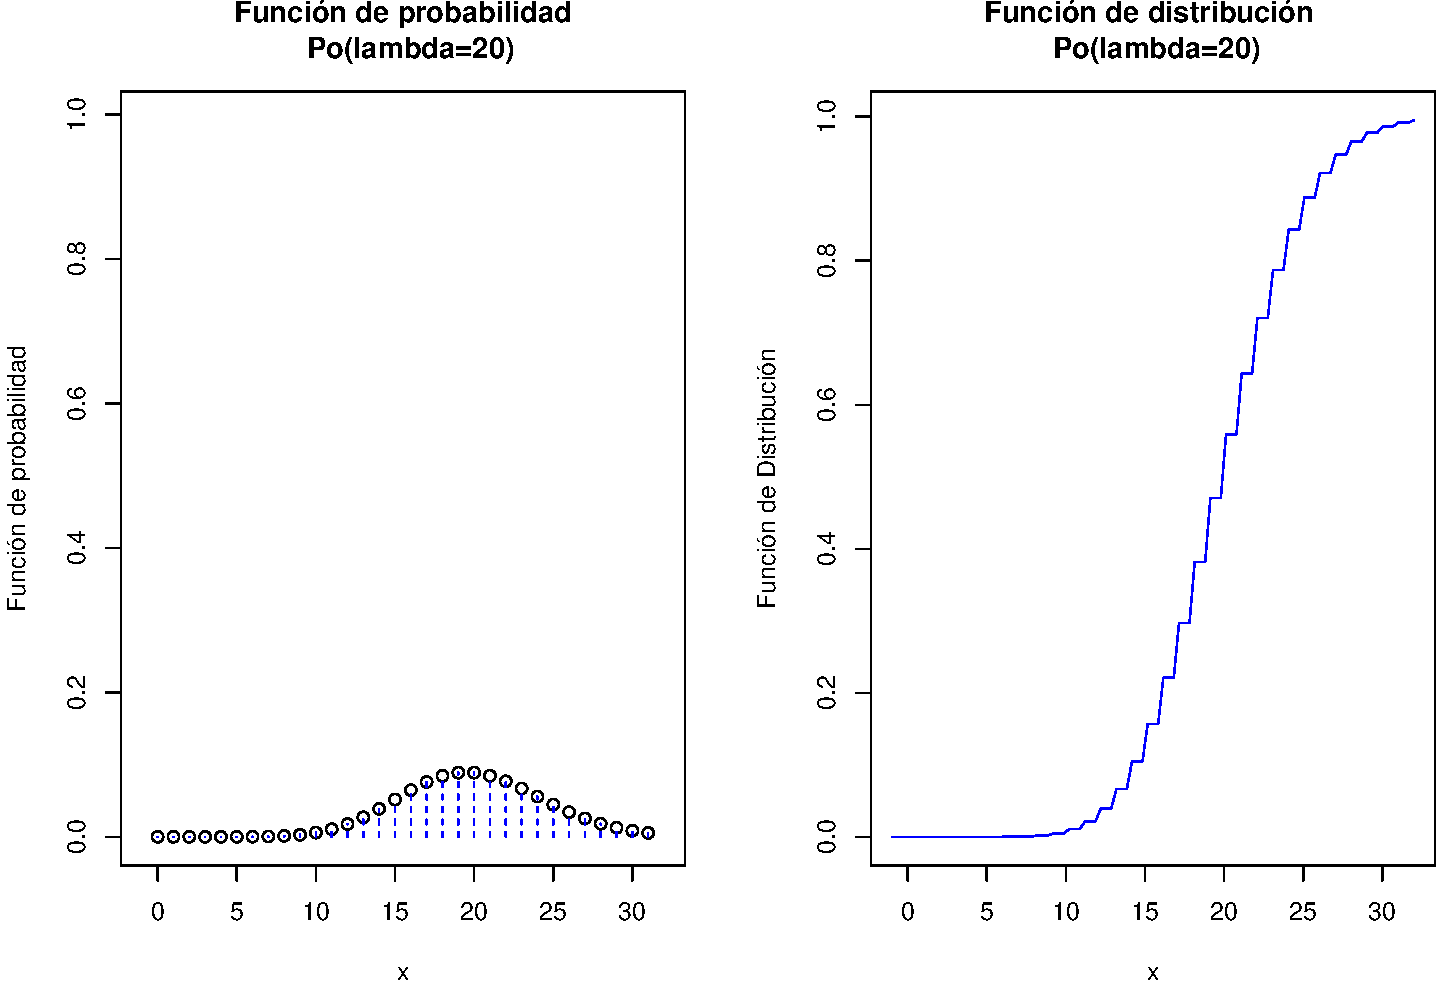
\includegraphics[width=0.8\textwidth,height=\textheight]{Tema_3_1_Notables_files/figure-beamer/graficosPOISON-1.pdf}

}

\end{figure}
\end{frame}

\begin{frame}[fragile]{Cálculos con python}
\protect\hypertarget{cuxe1lculos-con-python-4}{}
Sea \(X\) un una v.a. \(Po(\lambda=3)\). Entonces

\(P_X(0)=P(X=0), P_X(1)=P(X=1)\) en este orden son

\begin{Shaded}
\begin{Highlighting}[]
\ImportTok{from}\NormalTok{ scipy.stats }\ImportTok{import}\NormalTok{ poisson}
\NormalTok{poisson.pmf(}\DecValTok{0}\NormalTok{,mu }\OperatorTok{=} \DecValTok{3}\NormalTok{)}
\end{Highlighting}
\end{Shaded}

\begin{verbatim}
0.049787068367863944
\end{verbatim}

\begin{Shaded}
\begin{Highlighting}[]
\NormalTok{poisson.pmf(}\DecValTok{1}\NormalTok{,mu }\OperatorTok{=} \DecValTok{3}\NormalTok{)}
\end{Highlighting}
\end{Shaded}

\begin{verbatim}
0.14936120510359185
\end{verbatim}
\end{frame}

\begin{frame}[fragile]{Cálculos con python}
\protect\hypertarget{cuxe1lculos-con-python-5}{}
Sea \(X\) un una v.a. \(Po(\lambda=3)\). Entonces

\(F_X(0)=P(X\leq 0), F_X(1)=P(X\leq 1)\) en este orden son

\begin{Shaded}
\begin{Highlighting}[]
\NormalTok{poisson.cdf(}\DecValTok{0}\NormalTok{,mu }\OperatorTok{=} \DecValTok{3}\NormalTok{)}
\end{Highlighting}
\end{Shaded}

\begin{verbatim}
0.04978706836786395
\end{verbatim}

\begin{Shaded}
\begin{Highlighting}[]
\NormalTok{poisson.cdf(}\DecValTok{1}\NormalTok{,mu }\OperatorTok{=} \DecValTok{3}\NormalTok{)}
\end{Highlighting}
\end{Shaded}

\begin{verbatim}
0.1991482734714558
\end{verbatim}

\begin{Shaded}
\begin{Highlighting}[]
\NormalTok{poisson.pmf(}\DecValTok{0}\NormalTok{,mu }\OperatorTok{=} \DecValTok{3}\NormalTok{)}\OperatorTok{+}\NormalTok{poisson.pmf(}\DecValTok{1}\NormalTok{,mu}\OperatorTok{=} \DecValTok{3}\NormalTok{) }
\end{Highlighting}
\end{Shaded}

\begin{verbatim}
0.1991482734714558
\end{verbatim}

\begin{Shaded}
\begin{Highlighting}[]
\CommentTok{\#\# es igual a poisson.cdf(1,lambda=3)}
\end{Highlighting}
\end{Shaded}
\end{frame}

\begin{frame}[fragile]{Cálculos con python}
\protect\hypertarget{cuxe1lculos-con-python-6}{}
Por ejemplo podemos comprobar que
\(F_X(10)=\displaystyle\sum_{0}^{10} P_X(x)\)

\begin{Shaded}
\begin{Highlighting}[]
\NormalTok{poisson.pmf(}\BuiltInTok{range}\NormalTok{(}\DecValTok{0}\NormalTok{,}\DecValTok{10}\NormalTok{),mu}\OperatorTok{=}\DecValTok{3}\NormalTok{)}
\end{Highlighting}
\end{Shaded}

\begin{verbatim}
array([0.04978707, 0.14936121, 0.22404181, 0.22404181, 0.16803136,
       0.10081881, 0.05040941, 0.02160403, 0.00810151, 0.0027005 ])
\end{verbatim}

\begin{Shaded}
\begin{Highlighting}[]
\BuiltInTok{sum}\NormalTok{(poisson.pmf(}\BuiltInTok{range}\NormalTok{(}\DecValTok{0}\NormalTok{,}\DecValTok{10}\NormalTok{),mu}\OperatorTok{=}\DecValTok{3}\NormalTok{))}
\end{Highlighting}
\end{Shaded}

\begin{verbatim}
0.9988975118698846
\end{verbatim}

\begin{Shaded}
\begin{Highlighting}[]
\NormalTok{poisson.cdf(}\DecValTok{10}\NormalTok{,mu}\OperatorTok{=}\DecValTok{3}\NormalTok{)}
\end{Highlighting}
\end{Shaded}

\begin{verbatim}
0.9997076630493527
\end{verbatim}
\end{frame}

\begin{frame}[fragile]{Cálculos con python}
\protect\hypertarget{cuxe1lculos-con-python-7}{}
En el ejercicio de la trampa para insectos teníamos que \(X\) es una
\(Po(20)\). Responded con python a la preguntas 3 y 4 de este ejercicio

\textbf{Pregunta 3.} Calculad la probabilidad de que en una hora caigan
en la trampa exactamente 21 insectos.

La respuesta a la pregunta 3 es calcular \(P(X=21)\)

\begin{Shaded}
\begin{Highlighting}[]
\NormalTok{poisson.pmf(}\DecValTok{21}\NormalTok{,mu}\OperatorTok{=}\DecValTok{20}\NormalTok{)}
\end{Highlighting}
\end{Shaded}

\begin{verbatim}
0.08460506418293791
\end{verbatim}

\begin{Shaded}
\begin{Highlighting}[]
\CommentTok{\# P(X=21)}
\end{Highlighting}
\end{Shaded}
\end{frame}

\begin{frame}[fragile]{Cálculos con python}
\protect\hypertarget{cuxe1lculos-con-python-8}{}
\textbf{Pregunta 4.} Calculad la probabilidad de que en una hora caigan
en la trampa al menos 6 insectos.

La pregunta 4 nos pide calcular \(P(X\geq 6)=1-P(X\leq 5)\)

\begin{Shaded}
\begin{Highlighting}[]
\DecValTok{1}\OperatorTok{{-}}\NormalTok{poisson.cdf(}\DecValTok{5}\NormalTok{,mu}\OperatorTok{=}\DecValTok{20}\NormalTok{) }
\end{Highlighting}
\end{Shaded}

\begin{verbatim}
0.9999280911594716
\end{verbatim}

\begin{Shaded}
\begin{Highlighting}[]
\CommentTok{\# es 1{-}P(X\textless{}=5)=P(X\textgreater{}=6)}
\end{Highlighting}
\end{Shaded}
\end{frame}

\begin{frame}[fragile]{Cálculos con python}
\protect\hypertarget{cuxe1lculos-con-python-9}{}
Como ya hemos visto con \texttt{scipy.stats} podemos pedir los momentos
de una variable aleatoria \(Po(3)\)

\begin{Shaded}
\begin{Highlighting}[]
\NormalTok{poisson.stats(mu}\OperatorTok{=}\DecValTok{3}\NormalTok{, moments}\OperatorTok{=}\StringTok{\textquotesingle{}mv\textquotesingle{}}\NormalTok{)}
\end{Highlighting}
\end{Shaded}

\begin{verbatim}
(3.0, 3.0)
\end{verbatim}

Y también generar secuencias de observaciones aleatorias de una
población \(Po(3)\)

\begin{Shaded}
\begin{Highlighting}[]
\NormalTok{poisson.rvs(mu}\OperatorTok{=}\DecValTok{3}\NormalTok{,size}\OperatorTok{=}\DecValTok{40}\NormalTok{)}
\end{Highlighting}
\end{Shaded}

\begin{verbatim}
array([4, 1, 2, 0, 4, 3, 4, 3, 3, 5, 2, 2, 3, 2, 5, 3, 4, 5, 1, 3, 3, 2,
       3, 2, 3, 0, 2, 2, 2, 6, 2, 2, 1, 3, 1, 2, 1, 4, 4, 3], dtype=int64)
\end{verbatim}
\end{frame}

\begin{frame}[fragile]{Gráficos con python}
\protect\hypertarget{gruxe1ficos-con-python-2}{}
\begin{Shaded}
\begin{Highlighting}[]
\ImportTok{from}\NormalTok{ scipy.stats }\ImportTok{import}\NormalTok{ poisson}
\NormalTok{mu }\OperatorTok{=} \DecValTok{10} \CommentTok{\# mu = lambda}
\NormalTok{x }\OperatorTok{=}\NormalTok{ np.arange(poisson.ppf(}\FloatTok{0.01}\NormalTok{, mu),poisson.ppf(}\FloatTok{0.99}\NormalTok{, mu))}
\NormalTok{fig }\OperatorTok{=}\NormalTok{plt.figure(figsize}\OperatorTok{=}\NormalTok{(}\DecValTok{5}\NormalTok{, }\FloatTok{2.7}\NormalTok{))}
\NormalTok{ax }\OperatorTok{=}\NormalTok{ fig.add\_subplot(}\DecValTok{1}\NormalTok{,}\DecValTok{2}\NormalTok{,}\DecValTok{1}\NormalTok{)}
\NormalTok{ax.plot(x, poisson.pmf(x, mu), }\StringTok{\textquotesingle{}bo\textquotesingle{}}\NormalTok{, ms}\OperatorTok{=}\DecValTok{5}\NormalTok{, label}\OperatorTok{=}\StringTok{\textquotesingle{}poisson pmf\textquotesingle{}}\NormalTok{)}
\NormalTok{ax.vlines(x, }\DecValTok{0}\NormalTok{, poisson.pmf(x, mu), colors}\OperatorTok{=}\StringTok{\textquotesingle{}b\textquotesingle{}}\NormalTok{, lw}\OperatorTok{=}\DecValTok{2}\NormalTok{, alpha}\OperatorTok{=}\FloatTok{0.5}\NormalTok{)}
\ControlFlowTok{for}\NormalTok{ tick }\KeywordTok{in}\NormalTok{ ax.xaxis.get\_major\_ticks():}
\NormalTok{  tick.label.set\_fontsize(}\DecValTok{5}\NormalTok{)}
\ControlFlowTok{for}\NormalTok{ tick }\KeywordTok{in}\NormalTok{ ax.yaxis.get\_major\_ticks(): }
\NormalTok{  tick.label.set\_fontsize(}\DecValTok{5}\NormalTok{) }
\end{Highlighting}
\end{Shaded}
\end{frame}

\begin{frame}[fragile]{Gráficos con python}
\protect\hypertarget{gruxe1ficos-con-python-3}{}
\begin{Shaded}
\begin{Highlighting}[]
\NormalTok{ax }\OperatorTok{=}\NormalTok{ fig.add\_subplot(}\DecValTok{1}\NormalTok{,}\DecValTok{2}\NormalTok{,}\DecValTok{2}\NormalTok{)}
\NormalTok{ax.plot(x, poisson.cdf(x, mu), }\StringTok{\textquotesingle{}bo\textquotesingle{}}\NormalTok{, ms}\OperatorTok{=}\DecValTok{5}\NormalTok{, label}\OperatorTok{=}\StringTok{\textquotesingle{}poisson cdf\textquotesingle{}}\NormalTok{)}
\NormalTok{ax.vlines(x, }\DecValTok{0}\NormalTok{, poisson.cdf(x, mu), colors}\OperatorTok{=}\StringTok{\textquotesingle{}b\textquotesingle{}}\NormalTok{, lw}\OperatorTok{=}\DecValTok{2}\NormalTok{, alpha}\OperatorTok{=}\FloatTok{0.5}\NormalTok{)}
\ControlFlowTok{for}\NormalTok{ tick }\KeywordTok{in}\NormalTok{ ax.xaxis.get\_major\_ticks():}
\NormalTok{  tick.label.set\_fontsize(}\DecValTok{5}\NormalTok{)}
\ControlFlowTok{for}\NormalTok{ tick }\KeywordTok{in}\NormalTok{ ax.yaxis.get\_major\_ticks():}
\NormalTok{  tick.label.set\_fontsize(}\DecValTok{5}\NormalTok{)}
\NormalTok{fig.suptitle(}\StringTok{\textquotesingle{}Distribucion de Poisson\textquotesingle{}}\NormalTok{)}
\NormalTok{plt.show()}
\end{Highlighting}
\end{Shaded}
\end{frame}

\begin{frame}{Gráficos con python}
\protect\hypertarget{gruxe1ficos-con-python-4}{}
\begin{figure}

{\centering 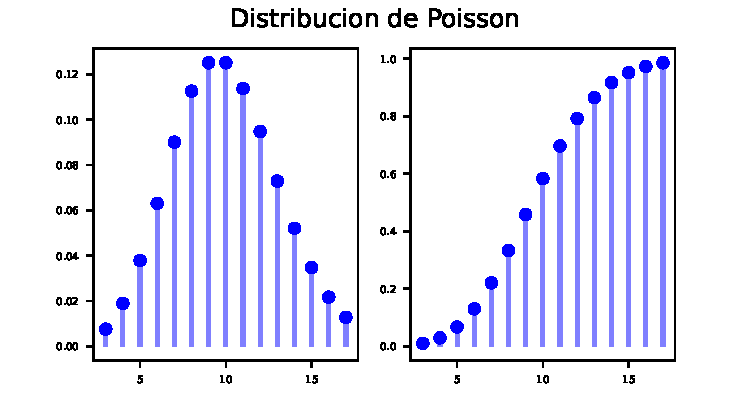
\includegraphics[width=0.7\textwidth,height=\textheight]{Tema_3_1_Notables_files/figure-beamer/py_poiss2_plot-1.pdf}

}

\end{figure}
\end{frame}

\begin{frame}{Ejemplo proceso Poisson}
\protect\hypertarget{ejemplo-proceso-poisson}{}
\textbf{Número de impactos de insectos en la visera de un casco}

Un colega de trabajo, al que llamaremos JG, es muy aficionado a los
grandes premios de velocidad tanto en coches como en motos.

Como es tan aficionado está obsesionado con muchas de las más
extravagantes estadísticas de estos deportes. En particular le
propusimos que estudiara el número de insectos que chocan contra la
visera de un casco de un motorista GP o de un conductor de fórmula 1 .
\end{frame}

\begin{frame}{Ejemplo proceso Poisson}
\protect\hypertarget{ejemplo-proceso-poisson-1}{}
La idea es que el número de insectos está igualmente repartido por todo
el circuito y de promedio impactan \(\lambda>0\) insectos por minuto.
También es razonable suponer que:

\begin{itemize}
\tightlist
\item
  podemos dividir la superficie de la visera en cuadrados
  suficientemente pequeños de forma que la probabilidad de que caigan
  dos insectos en la misma zona es prácticamente 0.
\item
  la probabilidad de que un insecto impacte en un cuadrado cualquiera de
  la visera es independiente de cualquier otro cuadrado.
\item
  si hemos dividido la visera en \(n\) cuadrados la probabilidad \(p_n\)
  de impacto de un cuadrado vale \(p_n=\frac{\lambda}{n}\).
\end{itemize}

Bajo estas condiciones, si denotamos por \(X_t\) como el número de
insectos que ha impactado en la visera en el intervalo \((0,t]\) (en
\(t\) minutos), podemos afirmar que \(X_t\) es un proceso de Poisson
\(Po(\lambda\cdot t)\).
\end{frame}

\begin{frame}[fragile]{Ejemplo proceso Poisson}
\protect\hypertarget{ejemplo-proceso-poisson-2}{}
Supongamos que nos dicen que \(\lambda=3\) insectos por minuto. Entonces
el proceso de poisson \(X_t\) seguirá un ley \(Po(3\cdot t).\)

Ahora estamos en condiciones de preguntar al proceso de Poisson.

¿Cuál es la probabilidad de que en 10 minutos impacten más de 25
insectos?

En este caso \(t=10\) \(X_{10}\)= número de insectos que impactan en 10
minutos, el intervalo \([0,10)\) que sigue una \(P(3\cdot 10=30)\). Por
lo tanto

\[P(X>25)=1-P(X\leq 25)\]

lo resolvemos con R

\begin{Shaded}
\begin{Highlighting}[]
\DecValTok{1}\SpecialCharTok{{-}}\FunctionTok{ppois}\NormalTok{(}\DecValTok{25}\NormalTok{,}\AttributeTok{lambda=}\DecValTok{30}\NormalTok{)}
\end{Highlighting}
\end{Shaded}

\begin{verbatim}
[1] 0.7916426
\end{verbatim}
\end{frame}

\begin{frame}[fragile]{Ejemplo proceso Poisson}
\protect\hypertarget{ejemplo-proceso-poisson-3}{}
Otra pregunta interesante es que tengamos que esperar más de 2 minutos
para observar el primer impacto

\[P(X_2=0)=\frac{(3\cdot 2)^0}{0!}\cdot e^{-3\cdot 2}= e^{-6}=0.002479.\]

Con R

\begin{Shaded}
\begin{Highlighting}[]
\DecValTok{6}\SpecialCharTok{\^{}}\DecValTok{0}\SpecialCharTok{/}\FunctionTok{factorial}\NormalTok{(}\DecValTok{0}\NormalTok{)}\SpecialCharTok{*}\FunctionTok{exp}\NormalTok{(}\SpecialCharTok{{-}}\DecValTok{6}\NormalTok{)}
\end{Highlighting}
\end{Shaded}

\begin{verbatim}
[1] 0.002478752
\end{verbatim}

\begin{Shaded}
\begin{Highlighting}[]
\FunctionTok{ppois}\NormalTok{(}\DecValTok{0}\NormalTok{,}\AttributeTok{lambda=}\DecValTok{3}\SpecialCharTok{*}\DecValTok{2}\NormalTok{)}
\end{Highlighting}
\end{Shaded}

\begin{verbatim}
[1] 0.002478752
\end{verbatim}
\end{frame}

\hypertarget{distribuciuxf3n-hipergeomuxe9trica}{%
\section{Distribución
hipergeométrica}\label{distribuciuxf3n-hipergeomuxe9trica}}

\begin{frame}{Modelo de la distribución hipergeométrica}
\protect\hypertarget{modelo-de-la-distribuciuxf3n-hipergeomuxe9trica}{}
Supongamos que disponemos de una urna de de sorteos que contiene \(m\)
bolas blancas y \(n\) bolas rojas.

En total en esta urna hay \(m+n\) bolas, \(m\) blancas y \(n\) rojas. Si
extraemos dos bolas de la urna lo podemos hacer de dos formas:

\begin{itemize}
\tightlist
\item
  Extraer una anotar su color y reponerla. Sacar otra y anotar su color.
  Hemos extraído la bola con reposición.
\item
  Extraer simultáneamente dos bolas (sin reposición) y contar el número
  de bolas blancas.
\end{itemize}
\end{frame}

\begin{frame}{Modelo de la distribución hipergeométrica}
\protect\hypertarget{modelo-de-la-distribuciuxf3n-hipergeomuxe9trica-1}{}
Sea \(X\) es la v.a. que cuenta el número de bolas blancas extraídas.

\begin{itemize}
\tightlist
\item
  En el primer caso, \(X\) es una \(B(n=2,p=\frac{m}{m+n})\) ya que
  consiste en repetir dos veces el mismo experimento de Bernoulli.
\item
  En el segundo caso, \(X\) sigue una distribución hipergeométrica que
  estudiaremos en esta sección.
\end{itemize}
\end{frame}

\begin{frame}{Modelo de la distribución hipergeométrica}
\protect\hypertarget{modelo-de-la-distribuciuxf3n-hipergeomuxe9trica-2}{}
Distribución hipergeométrica

Sean \(n\), \(m\) y \(k\) tres número enteros positivos y tales que
\(k<m+n\).

Consideremos una urna que contiene \(m+n\) bolas de las que \(m\) son
blancas y las restantes \(n\) no (son no blancas).

El número total de bolas es \(m+n\). Extraemos de forma aleatoria \(k\)
bolas de la urna sin reemplazarlas.
\end{frame}

\begin{frame}{Modelo de la distribución hipergeométrica}
\protect\hypertarget{modelo-de-la-distribuciuxf3n-hipergeomuxe9trica-3}{}
Sea \(X\) la v.a. que cuenta el número de bolas blancas extraídas.
Diremos que la distribución de \(X\) es hipergeométrica de parámetros
\(m\), \(n\) y \(k\) y la denotaremos por \(H(m,n,k)\).

Su dominio es

\[D_X=\left\{x\in\mathbf{N}\mid \max\{0,k-n\}\leq  x \leq \min\{m,k\}\right\}\]

Para explicarlo, veamos varios ejemplos:

\begin{itemize}
\tightlist
\item
  \(H(m=5,n=2,k=3)\). Tenemos \(m=5\) bolas blancas, \(n=2\) no blancas
  y sacamos \(k=3\) bolas sin reposición.

  \begin{itemize}
  \tightlist
  \item
    En este caso el mínimo de bolas blancas extraídas es \(1=k-n=3-2\),
    ya que sólo hay dos no blancas.
  \item
    En cambio, el máximo si es \(k=3\), ya que tenemos bolas blancas de
    ``sobra''.
  \end{itemize}
\end{itemize}
\end{frame}

\begin{frame}{Modelo de la distribución hipergeométrica}
\protect\hypertarget{modelo-de-la-distribuciuxf3n-hipergeomuxe9trica-4}{}
\[D_X=\left\{x\in\mathbf{N}\mid \max\{0,k-n\}\leq  x \leq \min\{m,k\}\right\}\]

\begin{itemize}
\tightlist
\item
  \(H(m=2,n=5,k=3)\). Tenemos \(m=2\) bolas blancas, \(n=5\) no blancas
  y sacamos \(k=3\) bolas sin reposición.

  \begin{itemize}
  \tightlist
  \item
    En este caso el mínimo de bolas blancas es \(0\) ya que puedo sacar
    3 no blancas.
  \item
    En cambio, el máximo si es \(m=2\), ya que aunque saquemos \(k=3\)
    bolas, al llegar a 2 ya hemos extraído todas las bolas blancas de la
    urna.
  \end{itemize}
\item
  \(H(m=10,n=10,k=3)\). Tenemos \(m=10\) bolas blancas, \(n=10\) no
  blancas y sacamos \(k=3\) bolas sin reposición.

  \begin{itemize}
  \tightlist
  \item
    En este caso podemos obtener desde \(0\) blancas hasta \(k=3\)
    blancas.
  \end{itemize}
\end{itemize}
\end{frame}

\begin{frame}{Modelo de la distribución hipergeométrica}
\protect\hypertarget{modelo-de-la-distribuciuxf3n-hipergeomuxe9trica-5}{}
Su función de probabilidad es:

Su función de probabilidad es: \[
P_{X}(x)=\left\{
\begin{array}{ll}
\frac{\binom{m}{x}\cdot \binom{n}{k-x}}{\binom{m+n}{k}}, & \mbox{ si }
\max\{0,k-n\}\leq x \leq \min\{m,k\}, \mbox { para  } x\in \mathbf{N},\\
0,  & \mbox{en otro caso.}\end{array}\right.
\]
\end{frame}

\begin{frame}{Distribución hipergeométrica}
\protect\hypertarget{distribuciuxf3n-hipergeomuxe9trica-1}{}
\textbf{Observación: otras parametrizaciones}

En ocasiones se parametriza una v.a. hipergeométrica mediante \(N=m+n\),
número total de bolas, \(k\), número de extracciones y \(p\),
probabilidad de extraer una bola blanca.

Así podemos \textbf{parametrizar alternativamente} la distribución
hipergeométrica así

\[H(N,k,p)\mbox{ donde } p=\frac{m}{N}.\]
\end{frame}

\begin{frame}{Resumen distribución Hipergeométrica \(H(m,n,k)\).}
\protect\hypertarget{resumen-distribuciuxf3n-hipergeomuxe9trica-hmnk.}{}
\renewcommand{\arraystretch}{1.75}
\begin{table}
\centering
\begin{tabular}{|l|}
\hline\rowcolor{LightBlue}
$X= \left\{\begin{array}{l}
\mbox{número de bolas blancas  en $k$ extracciones}\\
\mbox{sin reposición de una urna con} $m$\\
\mbox{bolas blancas y }$n$ \mbox{ negras.}
\end{array}\right.$;  $H(m,n,k)$
\\\hline
$D_X=\left\{x\in\mathbb{N}\mid \max\{0,k-n\}\leq  x \leq \min\{m,k\}\right\}$\\\hline
$P_X(x)=P(X=x)=\left\{
\begin{array}{ll}
\frac{\binom{m}{x}\cdot \binom{n}{k-x}}{\binom{m+n}{k}}, & \mbox{ si }
\max\{0,k-n\}\leq x \leq \min\{m,k\}, \\
0,  & \mbox{en otro caso.}\end{array}\right.$\\\hline
$F_X(x)=P(X\leq x)$.\\\hline
$E(X)=\frac{k\cdot m}{m+n}$; $Var(X)=k\cdot\frac{m}{m+n}\cdot\left(1-\frac{m}{m+n}\right) \cdot\frac{m+n-k}{m+n-1}$
\\\hline
\end{tabular}
\end{table}
\end{frame}

\begin{frame}{Ejemplo clásico urna \(m=15\) blancas, \(n=10\) rojas y
\(k=3\) extracciones sin reposición.}
\protect\hypertarget{ejemplo-cluxe1sico-urna-m15-blancas-n10-rojas-y-k3-extracciones-sin-reposiciuxf3n.}{}
\textbf{Urna con bolas blancas y rojas}

Tenemos una urna con 15 bolas blancas y 10 bolas rojas. Extraemos al
azar tres bolas de la urna sin reposición. Sea \(X\) el número de bolas
\textbf{blancas} extraídas. Bajo esta condiciones, la v.a. \(X\) sigue
una ley de distribución \(H(m=15,n=10,k=3)\).

La función de probabilidad es

\[
P_X(x)=P(X=x)=\left\{
\begin{array}{ll}
\frac{\binom{m}{x}\cdot \binom{n}{k-x}}{\binom{m+n}{k}} & \mbox{ si }
\max\{0,k-n\}\leq x \leq \min\{m,k\} \mbox { para  } x\in \mathbf{N}\\
0  & \mbox{en otro caso}\end{array}\right.,
\]

\[\mbox{sustituyendo }\scriptsize{
P_X(x)=P(X=x)=\left\{
\begin{array}{ll}
\frac{\binom{15}{x}\cdot \binom{10}{3-x}}{\binom{25}{3}} & \mbox{ si }
0\leq x \leq 3 \mbox { para  } x\in \mathbf{N}\\
0  & \mbox{en otro caso}\end{array}\right.
}\]
\end{frame}

\begin{frame}[fragile]{Ejemplo clásico urna \(m=15\) blancas, \(n=10\)
rojas y \(k=3\) extracciones sin reposición.}
\protect\hypertarget{ejemplo-cluxe1sico-urna-m15-blancas-n10-rojas-y-k3-extracciones-sin-reposiciuxf3n.-1}{}
La probabilidad de sacar 2 blancas será

\[
P(X=2)=\frac{\binom{15}{2}\cdot \binom{10}{3-2}}{\binom{25}{3}}
\]

\begin{Shaded}
\begin{Highlighting}[]
\FunctionTok{c}\NormalTok{(}\FunctionTok{choose}\NormalTok{(}\DecValTok{15}\NormalTok{,}\DecValTok{2}\NormalTok{), }\FunctionTok{choose}\NormalTok{(}\DecValTok{10}\NormalTok{,}\DecValTok{1}\NormalTok{), }\FunctionTok{choose}\NormalTok{(}\DecValTok{25}\NormalTok{,}\DecValTok{3}\NormalTok{))}
\end{Highlighting}
\end{Shaded}

\begin{verbatim}
[1]  105   10 2300
\end{verbatim}

\(P(X=2)=\frac{105\cdot10 }{2300}=0.4565217.\)
\end{frame}

\begin{frame}{Ejemplo clásico urna \(m=15\) blancas, \(n=10\) rojas y
\(k=3\) extracciones sin reposición.}
\protect\hypertarget{ejemplo-cluxe1sico-urna-m15-blancas-n10-rojas-y-k3-extracciones-sin-reposiciuxf3n.-2}{}
La probabilidad de que saquemos más de 1 bola blanca es

\[
\begin{array}{rl}
P(X> 1)&= 1-P(X\leq 1)=1-(P(X=0)+P(X=1))\\
&=
1-\left(\frac{\binom{15}{0}\cdot \binom{10}{3}}{\binom{25}{3}}+
\frac{\binom{15}{1}\cdot \binom{10}{2}}{\binom{25}{3}}\right)\\
&=
1-\left(
\frac{1\cdot120 }{2300}+\frac{15\cdot45 }{2300}
\right)=1-\frac{120+15\cdot 45}{2300}=0.6543478.
\end{array}
\]
\end{frame}

\begin{frame}{Ejemplo clásico urna \(m=15\) blancas, \(n=10\) rojas y
\(k=3\) extracciones sin reposición.}
\protect\hypertarget{ejemplo-cluxe1sico-urna-m15-blancas-n10-rojas-y-k3-extracciones-sin-reposiciuxf3n.-3}{}
El número esperado de bolas blancas extraídas para una v.a. \(X\)
\(H(m=15,n=10,k=3)\) es

\[E(X)=\frac{k\cdot m}{m+n}=\frac{3\cdot 15}{15+10}=\frac{45}{35}=1.285714.\]

La varianza vale: \[
\begin{array}{rl}
Var(X)&=k\cdot\frac{m}{m+n}\cdot\left(1-\frac{m}{m+n}\right) \cdot\frac{m+n-k}{m+n-1}\\
&=3\cdot\frac{15}{15+10}\cdot\left(1-\frac{15}{15+10}\right) \cdot\frac{15+10-3}{15+10-1}\\
&=
3\cdot\frac{15}{25}\cdot\left(1-\frac{15}{25}\right) \cdot\frac{22}{24}= 
3\cdot\frac{15}{25}\cdot\frac{25-15}{25} \cdot\frac{22}{24}\\
&=
3\cdot\frac{15}{25}\cdot\frac{10}{25}\cdot\frac{22}{24}=0.66.
\end{array}
\]

Y por lo tanto su desviación típica es

\[
+\sqrt{Var(X)}=+\sqrt{0.66}=0.812404.
\]
\end{frame}

\begin{frame}[fragile]{Cálculos con R}
\protect\hypertarget{cuxe1lculos-con-r-9}{}
Sea \(X\) una v.a. \(H(m,n,k)\). La función de \texttt{R} para calcular
la función de probabilidad en un valor \(x\), \(P(X=x)\), es
\texttt{dhyper(x,m,n,k)} y para calcular la función de distribución en
un valor \(q\), \(P(X\leq q)\), es \texttt{phyper(q,m,n,k)}. Para
generar una muestra de valores que siga la distribución \(H(m,n,k)\),
hay que usar la función \texttt{rhyper(nn,m,n,k)} donde \texttt{nn} es
el número de observaciones aleatorias deseado de la muestra.

Por ejemplo, si \(X\) es una \(H(m=15,n=10,k=3)\), los valores de
\(P(X=2)\) y que \(P(X>1)=1-P(X\leq 1)\) son:
\end{frame}

\begin{frame}[fragile]{Cálculos con R}
\protect\hypertarget{cuxe1lculos-con-r-10}{}
\begin{Shaded}
\begin{Highlighting}[]
\FunctionTok{dhyper}\NormalTok{(}\AttributeTok{x=}\DecValTok{2}\NormalTok{,}\AttributeTok{m=}\DecValTok{15}\NormalTok{,}\DecValTok{10}\NormalTok{,}\AttributeTok{k=}\DecValTok{3}\NormalTok{)}
\end{Highlighting}
\end{Shaded}

\begin{verbatim}
[1] 0.4565217
\end{verbatim}

\begin{Shaded}
\begin{Highlighting}[]
\FunctionTok{phyper}\NormalTok{(}\AttributeTok{q=}\DecValTok{1}\NormalTok{,}\AttributeTok{m=}\DecValTok{15}\NormalTok{,}\AttributeTok{n=}\DecValTok{10}\NormalTok{,}\AttributeTok{k=}\DecValTok{3}\NormalTok{)}\CommentTok{\# sí, le han puesto q ya veremos el porqué}
\end{Highlighting}
\end{Shaded}

\begin{verbatim}
[1] 0.3456522
\end{verbatim}

\begin{Shaded}
\begin{Highlighting}[]
\DecValTok{1}\SpecialCharTok{{-}}\FunctionTok{phyper}\NormalTok{(}\AttributeTok{q=}\DecValTok{1}\NormalTok{,}\AttributeTok{m=}\DecValTok{15}\NormalTok{,}\AttributeTok{n=}\DecValTok{10}\NormalTok{,}\AttributeTok{k=}\DecValTok{3}\NormalTok{)}
\end{Highlighting}
\end{Shaded}

\begin{verbatim}
[1] 0.6543478
\end{verbatim}
\end{frame}

\begin{frame}[fragile]{Cálculos con R}
\protect\hypertarget{cuxe1lculos-con-r-11}{}
Una muestra aleatoria de este experimento de tamaño 200 sería:

\begin{Shaded}
\begin{Highlighting}[]
\FunctionTok{rhyper}\NormalTok{(}\AttributeTok{nn=}\DecValTok{200}\NormalTok{,}\AttributeTok{m=}\DecValTok{15}\NormalTok{,}\AttributeTok{n=}\DecValTok{10}\NormalTok{,}\AttributeTok{k=}\DecValTok{3}\NormalTok{)}
\end{Highlighting}
\end{Shaded}

\begin{verbatim}
  [1] 2 3 1 3 1 2 2 3 2 2 1 2 1 2 2 3 3 1 1 1 1 0 2 3 2 1 3 2 2 2 2 3 2 3 3 2 0
 [38] 1 2 1 3 2 2 3 2 3 2 2 3 2 3 1 2 2 2 2 3 2 2 1 3 2 2 3 1 2 2 2 2 2 3 0 2 0
 [75] 3 2 2 2 1 2 2 3 1 1 1 2 2 2 2 1 1 3 2 2 3 2 2 1 1 1 3 3 2 2 2 1 3 2 2 2 1
[112] 1 2 3 2 2 1 2 2 2 2 2 2 3 1 2 3 3 1 1 2 2 1 1 3 2 1 1 2 2 3 1 1 1 2 1 1 3
[149] 1 2 2 3 3 2 3 1 2 1 2 2 2 1 2 3 1 3 3 3 2 2 1 3 3 1 1 2 2 2 2 2 3 2 1 2 1
[186] 1 1 1 2 1 1 2 2 2 2 3 3 1 0 2
\end{verbatim}
\end{frame}

\begin{frame}{Gráficas con R}
\protect\hypertarget{gruxe1ficas-con-r}{}
\begin{figure}

{\centering 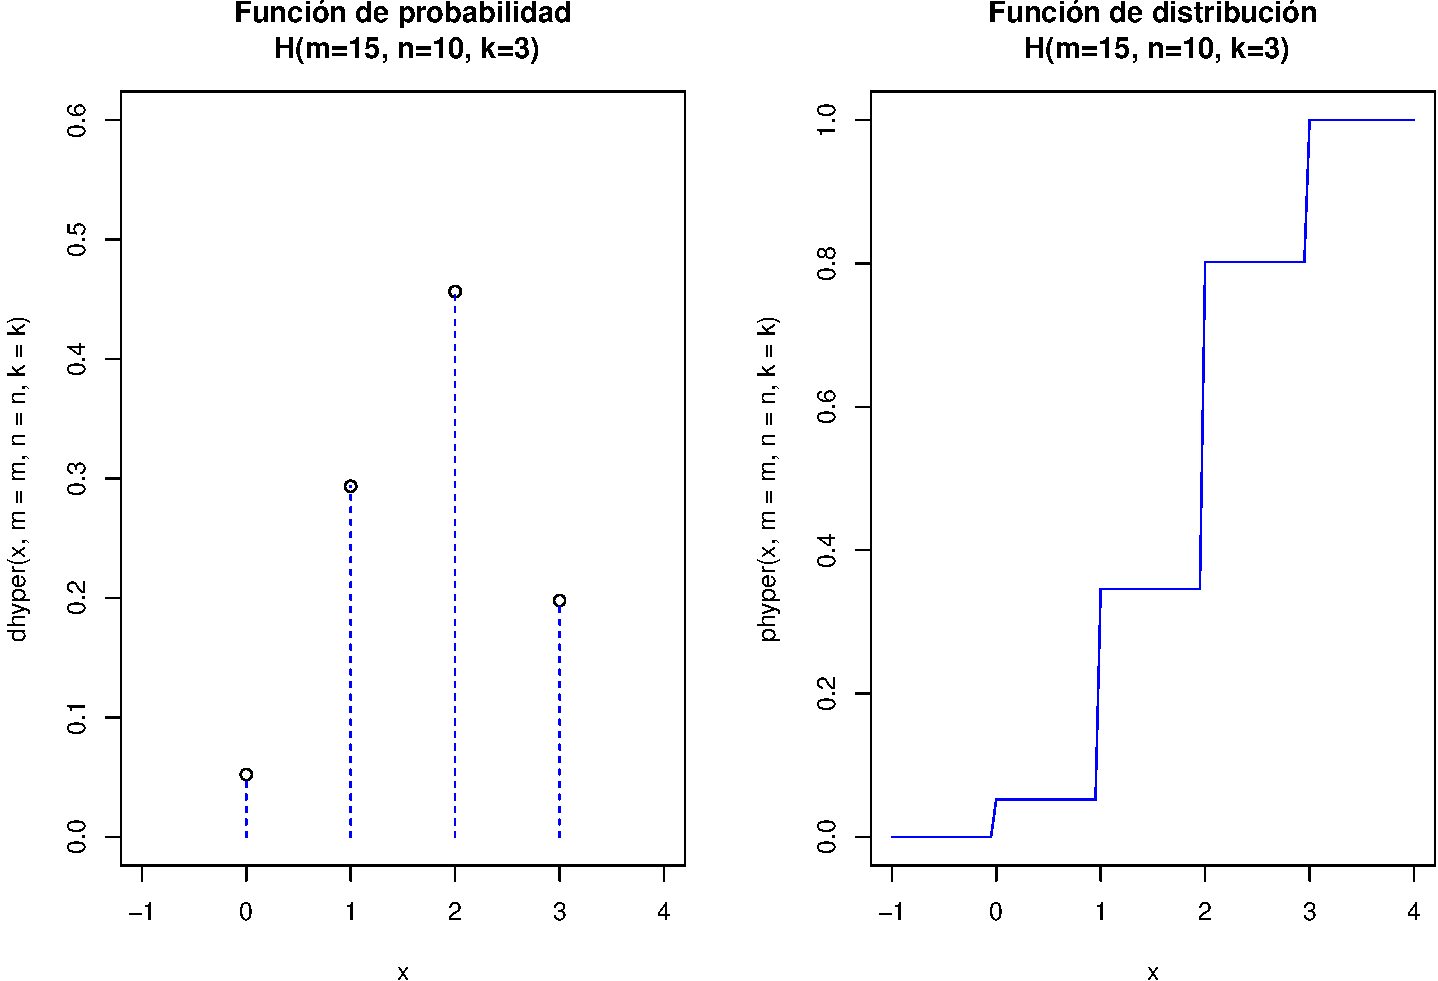
\includegraphics[width=0.7\textwidth,height=\textheight]{Tema_3_1_Notables_files/figure-beamer/unnamed-chunk-54-1.pdf}

}

\end{figure}
\end{frame}

\begin{frame}[fragile]{Cálculos con python}
\protect\hypertarget{cuxe1lculos-con-python-10}{}
Sea \(X\) una \(H(m,n,k)\), las funciones de \texttt{scipy.stats}
cambian los parámetros

\begin{itemize}
\tightlist
\item
  \(M\) es el número total de bolas. Con nuestra parametrización
  \(M=m+n\).
\item
  \(n\) es el número de bolas blancas. Con nuestra parametrización
  \(n=m\).
\item
  \(N\) es el número de extracciones. Con nuestra parametrización
  \(N=k\).
\end{itemize}

\begin{Shaded}
\begin{Highlighting}[]
\ImportTok{from}\NormalTok{ scipy.stats }\ImportTok{import}\NormalTok{ hypergeom}
\end{Highlighting}
\end{Shaded}
\end{frame}

\begin{frame}[fragile]{Cálculos con python}
\protect\hypertarget{cuxe1lculos-con-python-11}{}
\begin{Shaded}
\begin{Highlighting}[]
\NormalTok{hypergeom.pmf(}\DecValTok{1}\NormalTok{,M}\OperatorTok{=}\DecValTok{15}\OperatorTok{+}\DecValTok{10}\NormalTok{,n}\OperatorTok{=}\DecValTok{15}\NormalTok{,N}\OperatorTok{=}\DecValTok{3}\NormalTok{)}
\end{Highlighting}
\end{Shaded}

\begin{verbatim}
0.2934782608695652
\end{verbatim}

\begin{Shaded}
\begin{Highlighting}[]
\NormalTok{hypergeom.cdf(}\DecValTok{1}\NormalTok{,M}\OperatorTok{=}\DecValTok{15}\OperatorTok{+}\DecValTok{10}\NormalTok{,n}\OperatorTok{=}\DecValTok{15}\NormalTok{,N}\OperatorTok{=}\DecValTok{3}\NormalTok{)}
\end{Highlighting}
\end{Shaded}

\begin{verbatim}
0.3456521739130434
\end{verbatim}

\begin{Shaded}
\begin{Highlighting}[]
\DecValTok{1}\OperatorTok{{-}}\NormalTok{hypergeom.cdf(}\DecValTok{1}\NormalTok{,M}\OperatorTok{=}\DecValTok{15}\OperatorTok{+}\DecValTok{10}\NormalTok{,n}\OperatorTok{=}\DecValTok{15}\NormalTok{,N}\OperatorTok{=}\DecValTok{3}\NormalTok{)}
\end{Highlighting}
\end{Shaded}

\begin{verbatim}
0.6543478260869566
\end{verbatim}
\end{frame}

\begin{frame}[fragile]{Cálculos con python}
\protect\hypertarget{cuxe1lculos-con-python-12}{}
Una muestra aleatoria de este experimento sería\ldots{}

\begin{Shaded}
\begin{Highlighting}[]
\NormalTok{hypergeom.rvs(M}\OperatorTok{=}\DecValTok{15}\OperatorTok{+}\DecValTok{10}\NormalTok{,n}\OperatorTok{=}\DecValTok{15}\NormalTok{,N}\OperatorTok{=}\DecValTok{3}\NormalTok{,size}\OperatorTok{=}\DecValTok{100}\NormalTok{)}
\end{Highlighting}
\end{Shaded}

\begin{verbatim}
array([2, 2, 1, 2, 3, 3, 2, 2, 2, 2, 0, 3, 0, 2, 3, 2, 2, 3, 1, 2, 2, 0,
       3, 1, 1, 1, 2, 3, 1, 1, 2, 0, 2, 2, 0, 2, 2, 2, 3, 2, 1, 2, 1, 2,
       1, 1, 2, 1, 2, 1, 2, 1, 2, 2, 2, 2, 2, 1, 2, 2, 2, 2, 2, 2, 2, 1,
       2, 2, 2, 1, 0, 3, 1, 2, 2, 1, 2, 1, 0, 3, 2, 0, 2, 1, 3, 2, 3, 1,
       1, 1, 1, 2, 1, 0, 1, 3, 2, 1, 2, 1], dtype=int64)
\end{verbatim}
\end{frame}

\begin{frame}[fragile]{Gráficos con python}
\protect\hypertarget{gruxe1ficos-con-python-5}{}
\begin{Shaded}
\begin{Highlighting}[]
\ImportTok{from}\NormalTok{ scipy.stats }\ImportTok{import}\NormalTok{ hypergeom}
\NormalTok{[M, n, N] }\OperatorTok{=}\NormalTok{ [}\DecValTok{20}\NormalTok{, }\DecValTok{7}\NormalTok{, }\DecValTok{12}\NormalTok{] }\CommentTok{\#\#20 elementos, 7 del tipo, extraemos 12}
\NormalTok{x }\OperatorTok{=}\NormalTok{ np.arange(}\BuiltInTok{max}\NormalTok{(}\DecValTok{0}\NormalTok{, N}\OperatorTok{{-}}\NormalTok{M}\OperatorTok{+}\NormalTok{n),}\BuiltInTok{min}\NormalTok{(n, N))}
\NormalTok{fig }\OperatorTok{=}\NormalTok{plt.figure(figsize}\OperatorTok{=}\NormalTok{(}\DecValTok{5}\NormalTok{, }\FloatTok{2.7}\NormalTok{))}
 \OperatorTok{=}\NormalTok{ax }\OperatorTok{=}\NormalTok{ fig.add\_subplot(}\DecValTok{1}\NormalTok{,}\DecValTok{2}\NormalTok{,}\DecValTok{1}\NormalTok{)}
 \OperatorTok{=}\NormalTok{ax.plot(x, hypergeom.pmf(x, M, n, N), }\StringTok{\textquotesingle{}bo\textquotesingle{}}\NormalTok{, ms}\OperatorTok{=}\DecValTok{5}\NormalTok{, label}\OperatorTok{=}\StringTok{\textquotesingle{}hypergeom pmf\textquotesingle{}}\NormalTok{)}
 \OperatorTok{=}\NormalTok{ax.vlines(x, }\DecValTok{0}\NormalTok{, hypergeom.pmf(x, M, n, N), colors}\OperatorTok{=}\StringTok{\textquotesingle{}b\textquotesingle{}}\NormalTok{, lw}\OperatorTok{=}\DecValTok{2}\NormalTok{, alpha}\OperatorTok{=}\FloatTok{0.5}\NormalTok{)}
 \OperatorTok{=}\NormalTok{ax.set\_ylim([}\DecValTok{0}\NormalTok{, }\BuiltInTok{max}\NormalTok{(hypergeom.pmf(x, M, n, N))}\OperatorTok{*}\FloatTok{1.1}\NormalTok{])}
\end{Highlighting}
\end{Shaded}
\end{frame}

\begin{frame}[fragile]{Gráficos con python}
\protect\hypertarget{gruxe1ficos-con-python-6}{}
\begin{Shaded}
\begin{Highlighting}[]
\ControlFlowTok{for}\NormalTok{ tick }\KeywordTok{in}\NormalTok{ ax.xaxis.get\_major\_ticks():}
   \OperatorTok{=}\NormalTok{tick.label.set\_fontsize(}\DecValTok{5}\NormalTok{)}
\ControlFlowTok{for}\NormalTok{ tick }\KeywordTok{in}\NormalTok{ ax.yaxis.get\_major\_ticks():}
  \OperatorTok{=}\NormalTok{tick.label.set\_fontsize(}\DecValTok{5}\NormalTok{) }
\NormalTok{ax }\OperatorTok{=}\NormalTok{ fig.add\_subplot(}\DecValTok{1}\NormalTok{,}\DecValTok{2}\NormalTok{,}\DecValTok{2}\NormalTok{)}
 \OperatorTok{=}\NormalTok{ax.plot(x, hypergeom.cdf(x, M, n, N), }\StringTok{\textquotesingle{}bo\textquotesingle{}}\NormalTok{, ms}\OperatorTok{=}\DecValTok{5}\NormalTok{, label}\OperatorTok{=}\StringTok{\textquotesingle{}hypergeom cdf\textquotesingle{}}\NormalTok{)}
 \OperatorTok{=}\NormalTok{ax.vlines(x, }\DecValTok{0}\NormalTok{, hypergeom.cdf(x, M, n, N), colors}\OperatorTok{=}\StringTok{\textquotesingle{}b\textquotesingle{}}\NormalTok{, lw}\OperatorTok{=}\DecValTok{2}\NormalTok{, alpha}\OperatorTok{=}\FloatTok{0.5}\NormalTok{)}
\ControlFlowTok{for}\NormalTok{ tick }\KeywordTok{in}\NormalTok{ ax.xaxis.get\_major\_ticks():}
   \OperatorTok{=}\NormalTok{tick.label.set\_fontsize(}\DecValTok{5}\NormalTok{)}
\ControlFlowTok{for}\NormalTok{ tick }\KeywordTok{in}\NormalTok{ ax.yaxis.get\_major\_ticks():}
   \OperatorTok{=}\NormalTok{tick.label.set\_fontsize(}\DecValTok{5}\NormalTok{)}
 \OperatorTok{=}\NormalTok{fig.suptitle(}\StringTok{\textquotesingle{}Distribucion Hipergeometrica\textquotesingle{}}\NormalTok{)}
 \OperatorTok{=}\NormalTok{plt.show()}
\end{Highlighting}
\end{Shaded}
\end{frame}

\begin{frame}{Gráficos con python}
\protect\hypertarget{gruxe1ficos-con-python-7}{}
from scipy.stats import hypergeom {[}M, n, N{]} = {[}20, 7, 12{]} \#\#20
elementos, 7 del tipo, extraemos 12 x = np.arange(max(0, N-M+n),min(n,
N)) fig =plt.figure(figsize=(5, 2.7)) \emph{=ax =
fig.add\_subplot(1,2,1) }=ax.plot(x, hypergeom.pmf(x, M, n, N), `bo',
ms=5, label=`hypergeom pmf') \emph{=ax.vlines(x, 0, hypergeom.pmf(x, M,
n, N), colors=`b', lw=2, alpha=0.5) }=ax.set\_ylim({[}0,
max(hypergeom.pmf(x, M, n, N))*1.1{]}) for tick in
ax.xaxis.get\_major\_ticks(): \emph{=tick.label.set\_fontsize(5) for
tick in ax.yaxis.get\_major\_ticks(): }=tick.label.set\_fontsize(5) ax =
fig.add\_subplot(1,2,2) \emph{=ax.plot(x, hypergeom.cdf(x, M, n, N),
`bo', ms=5, label=`hypergeom cdf') }=ax.vlines(x, 0, hypergeom.cdf(x, M,
n, N), colors=`b', lw=2, alpha=0.5) for tick in
ax.xaxis.get\_major\_ticks(): \emph{=tick.label.set\_fontsize(5) for
tick in ax.yaxis.get\_major\_ticks(): }=tick.label.set\_fontsize(5)
\emph{=fig.suptitle(`Distribucion Hipergeometrica') }=plt.show()
\end{frame}



\end{document}
